\documentclass[11pt]{article}
\usepackage[margin=2.2cm]{geometry}
\usepackage{amsmath,amssymb,amsthm}
\usepackage{graphicx}
\usepackage{booktabs,array,tabularx}
\usepackage{float}
\usepackage{needspace}
\usepackage{placeins}
% Keep float-only pages top-aligned without stretching gaps between tables.
\makeatletter
\setlength{\@fptop}{0pt}
\setlength{\@fpsep}{12pt plus 2pt minus 2pt}
\setlength{\@fpbot}{0pt plus 1fil}
\makeatother
\renewcommand{\topfraction}{0.9}
\renewcommand{\bottomfraction}{0.9}
\renewcommand{\textfraction}{0.05}
\renewcommand{\floatpagefraction}{0.85}
\setcounter{topnumber}{3}
\setcounter{bottomnumber}{3}
\setcounter{totalnumber}{5}
\usepackage[super,sort&compress,comma]{natbib}
\usepackage[T1]{fontenc}
\usepackage{hyperref}
\hypersetup{
  hidelinks,
  pdftitle={Supporting Information for Increasing electricity exports through delivery-informed allocation in distribution networks},
  pdfauthor={Junjie Huang, Tao Yu, Zhenning Pan, Yufeng Wu, Wencong Xiao, Rankai Zhu, Jie Huang, and Yusheng Xue}
}
\newcommand{\indicator}{\mathbb{I}}
% Repository placeholder: replace the owner and add the final DOI before submission.
\newcommand{\repositoryurl}{\url{https://github.com/MarxHuang/ecf-export-access}}
\newtheorem{proposition}{Proposition}
\title{Supporting Information for\\[0.5em]
\textbf{Increasing electricity exports through delivery-informed allocation\\
in distribution networks}}
\author{Junjie Huang, Tao Yu, Zhenning Pan, Yufeng Wu,\\
Wencong Xiao, Rankai Zhu, Jie Huang, and Yusheng Xue}
\date{}
\begin{document}
\maketitle

This Supporting Information (SI) provides the mathematical and numerical basis
for three distinctions in the main paper: private delivery gains versus losses
elsewhere, total request reduction versus its distribution across participants, and
completed-state recovery versus later feedback performance. Part I derives
these relationships and the bounded ECF update. Part II specifies the allocation
rules and controlled network approximation. Part III describes the public-data
simulation and reports the complete energy, sensitivity, and topology results.
The tables retain detailed numerical results so that the main paper can focus
on their interpretation.

\renewcommand{\thesection}{S\arabic{section}}
\renewcommand{\theequation}{S\arabic{equation}}
\renewcommand{\thefigure}{S\arabic{figure}}
\renewcommand{\thetable}{S\arabic{table}}
\setcounter{section}{0}
\setcounter{equation}{0}

\section*{Part I. Mathematical Derivations}

\section{Guide to the Supporting Analyses and Notation}
\label{supp:scope}

The supporting analyses follow the argument from request choice to delivery
and then to feedback. Section S2 derives the distinction between private payoff
and total delivery. Sections S3--S4 define the temporal update and the equal-total
comparison. Sections S5--S9 supply allocation details, and Section S10 evaluates
the same feedback with public profiles and network models.
Table~\ref{tab:supp_experiment_evidence_map} provides a more detailed guide.
Shared symbols appear in Section S1.1; derivation-specific symbols and parameter
grids are defined locally. Throughout, $[\,\cdot\,]^+$ denotes the positive-part
operator.

The main paper generally reports power differences to one decimal place and
network energy totals to two, retaining additional digits for small effects
and numerical limits. Smaller energy differences are expressed in kWh rather
than MWh; $1~\mathrm{MWh}=1000~\mathrm{kWh}$. Tables here retain additional
precision, and all differences and percentages are calculated before rounding.
A request-effect difference is changed minus forecast-based reference requests;
a feedback difference is ECF minus the named control. These conventions apply
to the numerical tables throughout.

Controlled results refer to the stated case or trajectory grid. Australian
comparisons use paired network days. Section and model panels are reported at
their own spatial units rather than pooled into one network-population estimate.

\clearpage
\begin{table}[!ht]
\centering
\caption{Map from the main-paper questions to the supporting analyses}
\label{tab:supp_experiment_evidence_map}
\footnotesize
\setlength{\tabcolsep}{3.0pt}
\renewcommand{\arraystretch}{1.08}
\begin{tabularx}{\textwidth}{@{}>{\raggedright\arraybackslash}p{0.15\textwidth}>{\raggedright\arraybackslash}p{0.27\textwidth}>{\raggedright\arraybackslash}p{0.21\textwidth}>{\raggedright\arraybackslash}X@{}}
\toprule
Analysis & Purpose and principal comparison & Outcome and analysis unit & Interpretation and location \\
\midrule
Controlled request choice & Compares each selected multiplier
$\gamma_i^\star$ with the matched forecast-based request across five allocation
rules. & Request-choice case; delivery of the changed group, delivery elsewhere,
and total delivery in kW. & Separates productive larger requests from
request--access--delivery externalities; main Fig.~3 and Section~S2. \\
Controlled feedback & Compares ECF with the shortfall-cost benchmark,
mismatch-only feedback, and the equal-total control. & Sixteen-interval
trajectory; signed delivery change in kW. & Tests whether completed-state replay
and selective ceiling updates recover delivery; main Figs.~4--6 and Sections
S3--S4. \\
Controlled operating conditions & Varies feedback gain, allocation rule,
electrical location, and reactive-power setting. &
Matched interval pair; delivery, allocation equality, voltage, and two-ended
branch loading. & Retains positive, zero, and negative responses and verifies
all reported controlled states with the specified AC power-flow checks; main
Figs.~6--8 and Sections S3 and S9. \\
Australian replay & Compares ECF with no feedback, previous-day persistence,
and the equal-total control. & Paired network day; delivered energy and
source-terminal exchange in MWh. & Tests the targeting contrast using public
chronology and a published medium-/low-voltage (MV/LV) network; main Fig.~9 and
Section~S10. \\
Australian sensitivities & Varies feedback gain, available-export-record scale
and timing, unavailable records, and customer cohort. & Paired network day;
delivery contrast and physical-check status. & Tests sensitivity to the feedback
setting and constructed post-event record; main Fig.~10 and Section~S10. \\
Feedback components and memory & Removes replay qualification while retaining
the update formula; separately retains ceilings across consecutive dates. &
Paired network day and calendar-block energy differences. & Separates the
criterion's contribution from initialization effects; Sections S10.6 and S10.8. \\
Bounded records & Compares point-record and delivery-lower-bound control at
three radii and both common bias directions. & Paired network day, recovery
opportunities, and separately screened replay states. & Distinguishes recovery
qualification from later energy gains; Section S10.9. \\
Spatial and topology checks & Reassigns profiles in five ways, and examines
13 LV sections and nine representative LV models. & Mapping-, section-, or model-level delivery sign,
energy difference, qualifying-interval count, and physical-check status. & Shows how activation
and delivery recovery vary with electrical location and published topology;
main Fig.~11 and Sections S10.10 and S10.12--S10.13. \\
Individual delivery & Compares each participant's cumulative and daily delivery
under ECF and three controls. & Participant and participant-day differences. &
Distinguishes aggregate gains from their distribution; Section S10.14. \\
PV capacity & Scales PV at five levels while retaining participant locations
and profile assignment. & Paired network day, energy balance, and gain per
installed MW. & Tests whether the delivery advantage depends on the primary
capacity level; Section S10.11. \\
Request adaptation & Participants revise request-choice probabilities from
their own completed delivery; a fixed-probability comparison uses the same
candidates and random draws. & Paired network day after averaging three seeds;
separate controller histories and a conditional equal-total shadow. & Tests
whether ECF's delivery advantage persists under experience-based request
adjustment; Section S10.15. \\
Allocation-formulation checks & Varies retained network margin and the
fairness-aware (FA) objective weight outside the primary ECF comparison. &
Allocation movement, capacity-normalized Jain index, and matched AC feasibility.
& Describes formulation sensitivity; Sections S5--S6. \\
\bottomrule
\end{tabularx}
\end{table}

\subsection{Recurring Symbols}

The following table collects notation used in several sections. Symbols used in
only one derivation are defined where they first appear.
\begin{center}
\footnotesize
\renewcommand{\arraystretch}{1.05}
\begin{tabular}{@{}p{0.27\textwidth}p{0.67\textwidth}@{}}
\hline
Symbol & Meaning \\
\hline
$i,j,t,b,\ell;\ \mathcal N,\mathcal T,\mathcal B,\mathcal L$ & Participant indices $i,j$, interval index $t$, bus index $b$, branch index $\ell$, and their sets. \\
$\mathcal K,\mathcal G,\nu(i)$ & Changed-request set, distribution-network graph, and participant-to-bus map. \\
$\mathcal R,\mathcal M;\ \Pi_{\mathcal R},\mathcal F_{\mathcal M}$ & Allocation rule and network model; allocation and feasible-set maps. \\
$\mathbf z,\boldsymbol\xi_{\mathrm{net}},\boldsymbol\eta_{\mathcal R}$ & Exogenous network data, endogenous network variables, and rule parameters. \\
$r_i,r_i^{\mathrm{cap}},r_i^{\mathrm{adm}},x_i$ & Submitted, capacity-limited, and admitted requests, and authorized export access (MW). \\
$C_i,a_i^{\mathrm{fcst}},a_i,a_i^{\mathrm{prof}},a_i^{\mathrm{tel}},y_i$ & Connection bound, point forecast, available export, profile-derived available-export proxy, post-event replay record, and completed-interval delivery (MW). \\
$F_i(\cdot\mid s_i),\gamma_i;\ U_i,u_i,\vartheta$ & Conditional cumulative distribution function (CDF) of available export and request multiplier; expected/realized payoff and normalized shortfall-cost parameter. \\
$\mathcal N_{\mathrm{ua}}(t),g(t),\psi_i,\beta_{\mathrm{ECF}}$ & Unused-award group, indicator that all replay conditions hold, request ceiling, and ECF update gain. \\
$\mathbf r^{\mathrm{rpl}},\mathbf x^{\mathrm{rpl}},\mathbf y^{\mathrm{rpl}}$ & Completed-state replay request, access, and delivery vectors. \\
$X,Y,H,\Delta Y,M_x$ & Total authorized access, total completed delivery, total unused award, signed delivery change, and allocation movement (MW before conversion to the reported kW values). \\
$\mathcal V_b,v_b,S_{\ell,e},\bar S_{\ell}^{\mathrm{syn}}$ & AC voltage phasor and magnitude, branch-end complex power, and synthetic scenario rating. \\
WP, ER, EA, ME, FA & Weighted proportional, equal reduction, equal access, maximum export, and fairness-aware allocation. \\
ECF, MR & Externality-conditioned counterfactual feedback and margin retention. \\
\hline
\end{tabular}
\end{center}

Sections S2 and S4--S9 suppress $t$ after explicitly fixing one interval.
Sections S3 and S10 retain their interval or day/half-hour indices. The
participant set is $\mathcal N$.
Participant $i$ submits request $r_i$ and has connection bound $C_i>0$.
The private forecast is $a_i^{\mathrm{fcst}}$. In the controlled study,
$a_i$ is simulated available active-power export and authorized access $x_i$
gives delivery $y_i=\min\{x_i,a_i\}$. Its post-event replay record is exact,
$a_i^{\mathrm{tel}}=a_i$. The Australian study instead constructs the
profile-derived proxy $a_i^{\mathrm{prof}}$ from scaled gross-PV generation and
household consumption. It models control-dependent delivery as
$y_i^c=\min\{x_i^c,a_i^{\mathrm{prof}}\}$ and sets the primary replay record to
$a_i^{\mathrm{tel}}=a_i^{\mathrm{prof}}$. Record sensitivities alter only
$a_i^{\mathrm{tel}}$. Thus public-case delivery is a model outcome rather than
source-metered export. Section~S10 defines the construction and sensitivities.

The connection bound first gives
$r_i^{\mathrm{cap}}=\min\{r_i,C_i\}$. Externality-conditioned counterfactual
feedback (ECF) then applies the MW-valued ceiling
$\psi_i\in[0,C_i]$. The request presented to the allocation rule is
\begin{equation}
r_i^{\mathrm{adm}}=\min\{r_i^{\mathrm{cap}},\psi_i\}.
\label{eq:supp_credible_request}
\end{equation}
These quantities are successive request stages: submission, application of the
connection bound, and application of the ECF ceiling. Once $\psi_i$ binds, a
larger submitted request cannot increase $r_i^{\mathrm{adm}}$. Fixed-interval
derivations condition on the current ceiling. The gain
$\beta_{\mathrm{ECF}}$ affects allocation through the ceiling trajectory across
intervals. The behavioral model also includes a normalized shortfall cost, but
that cost enters request choice rather than the allocation map or ceiling
update.
The feeder graph and exogenous network data are $\mathcal G$ and $\mathbf z$,
respectively.

For allocation rule $\mathcal R$ and network model $\mathcal M$, the allocation
map is
\begin{equation}
\mathbf x^{\mathcal R,\mathcal M}
=\Pi_{\mathcal R}\!\left(
\mathbf r^{\mathrm{adm}};
\mathcal F_{\mathcal M}(\mathcal G,\mathbf z),
\boldsymbol\eta_{\mathcal R}\right).
\label{eq:supp_allocation_map}
\end{equation}
Without an active ECF ceiling, $\mathbf r^{\mathrm{adm}}=\mathbf r^{\mathrm{cap}}$.
Otherwise, the same allocation map receives the ceiling-limited request in
\eqref{eq:supp_credible_request}. Rule parameters
$\boldsymbol\eta_{\mathcal R}$ enter $\Pi_{\mathcal R}$. They do not alter the
network-feasible set. The auxiliary margin-retention variant is defined with its sensitivity
analysis in Section S5. Without an active ECF ceiling, $\psi_i=C_i$.

\section{Request Choice and Delivery Externality}
\label{supp:behavioral_diagnostic}

A request affects private payoff through the participant's own award, but
affects total delivery through awards at every connection. The derivation below
separates these paths using one conditional available-export model for both
request choice and delivery. Continuous-regime derivatives give the local
relationship; matched finite differences apply to the discrete output tree.
The numerical classification additionally requires an increased unused award,
as specified in Section S2.2.

Participant $i$ observes private signal $s_i$ and forms point forecast
$a_i^{\mathrm{fcst}}$. The conditional cumulative distribution function (CDF)
$F_i(\cdot\mid s_i)$ describes uncertainty in available export. Because the
connection bound $C_i$ clips the distribution, the point forecast need not equal
its clipped mean. Request, access, available export, and delivery obey
\begin{equation}
r_i(\gamma_i)=\gamma_i a_i^{\mathrm{fcst}},
\quad
x_i(\gamma_i)=[\Pi_{\mathcal R}(\mathbf r^{\mathrm{adm}}(\gamma_i))]_i,
\quad
y_i(\gamma_i)=\min\{x_i(\gamma_i),a_i\},
\qquad \gamma_i\ge1.
\label{eq:supp_behavior_chain}
\end{equation}
Here $a_i\sim F_i(\cdot\mid s_i)$. The same distribution therefore supports the
request decision and the later delivery realization. In a single-participant
comparison, all other participants retain their reference requests. This
construction generates internally consistent controlled requests; it is not an
equilibrium model of participant behavior.
Let $\vartheta\ge0$ denote the modeled cost per unit of unused award, normalized
by the value per unit of delivered export. The conditional expected payoff is
\begin{equation}
U_i(\gamma_i;\vartheta)
=\bar y_i(\gamma_i)-\vartheta\bar h_i(\gamma_i)
=\mathbb E\!\left[
\min\{x_i(\gamma_i),a_i\}
-\vartheta[x_i(\gamma_i)-a_i]^+
\mid s_i\right].
\label{eq:supp_behavioral_payoff}
\end{equation}
Here
$\bar y_i(\gamma_i)=\mathbb E[\min\{x_i(\gamma_i),a_i\}\mid s_i]$ and
$\bar h_i(\gamma_i)=\mathbb E[[x_i(\gamma_i)-a_i]^+\mid s_i]$.
For a realized outcome, the corresponding normalized payoff is
$u_i(t)=y_i(t)-\vartheta[x_i(t)-y_i(t)]^+$. Thus $U_i$ and $u_i$ denote
expected and realized quantities, respectively.
The expectation is over available export after the request and award have been
fixed. All derivatives below hold the conditional available-export CDFs and
exogenous inputs fixed. Conditional arguments are suppressed when no ambiguity
arises.
\subsection{Private-payoff and total-delivery effects}
\label{supp:full_private_feeder_proof}

For a CDF $F_i$ that is continuous at $x_i$,

\begin{equation}
\frac{\partial}{\partial x_i}
\mathbb E[\min\{x_i,a_i\}\mid s_i]
=1-F_i(x_i\mid s_i),
\qquad
\frac{\partial}{\partial x_i}
\mathbb E[(x_i-a_i)^+\mid s_i]
=F_i(x_i\mid s_i).
\label{eq:supp_expected_delivery_derivatives}
\end{equation}
To see the first identity, write
$\mathbb E[\min\{x_i,a_i\}]=\int_0^{x_i}[1-F_i(u)]\,du$ for nonnegative
available export. The second follows from
$\mathbb E[(x_i-a_i)^+]=\int_0^{x_i}F_i(u)\,du$. Applying the chain rule with
$J_{ji}=\partial x_j/\partial r_i$ proves the private gradient in the main
paper:
\begin{equation}
\frac{\partial U_i}{\partial r_i}
=J_{ii}\left[1-F_i(x_i)-\vartheta F_i(x_i)\right].
\label{eq:supp_private_request_gradient}
\end{equation}
If $J_{ii}>0$ and the optimum is interior, its target award satisfies
$F_i(x_i)=1/(1+\vartheta)$. A zero shortfall cost therefore values the upper
available-export tail, while a larger shortfall cost selects a lower award quantile.

For conditional expected aggregate metered delivery
$\bar Y=\sum_j\mathbb E[\min\{x_j,a_j\}\mid s_j]$, the same chain rule gives
\begin{equation}
\frac{\partial\bar Y}{\partial r_i}
=\sum_{j\in\mathcal N}J_{ji}[1-F_j(x_j)].
\label{eq:supp_feeder_request_gradient}
\end{equation}
Equating this derivative with the private-payoff derivative in
\eqref{eq:supp_private_request_gradient} gives
\begin{equation}
\vartheta_i^{\mathrm{ext}}
=-\frac{\sum_{j\ne i}J_{ji}[1-F_j(x_j)]}
{J_{ii}F_i(x_i)},
\qquad J_{ii}F_i(x_i)>0.
\label{eq:supp_externality_equivalent_shortfall_cost}
\end{equation}
Equation~\eqref{eq:supp_externality_equivalent_shortfall_cost} gives the
normalized shortfall cost that would locally align the participant's marginal
payoff with the marginal change in total delivery. This value depends on the
active allocation response, electrical location, competing requests, and
available-export CDFs. It may change when the active set changes and need not be
positive when access is slack. One fixed shortfall cost therefore cannot be
expected to reproduce every local cross-participant delivery effect. Settlement
and ECF are consequently evaluated as different interventions.
The participant internalizes only its own payoff derivative. Under scarcity,
some $J_{ji}$ for $j\ne i$ are negative. Hence the local delivery externality
condition is
\begin{equation}
\frac{\partial U_i}{\partial r_i}>0,
\qquad
\frac{\partial\bar Y}{\partial r_i}<0.
\label{eq:supp_delivery_externality_condition}
\end{equation}
The request-to-access Jacobian makes this local condition depend on the
allocation rule. The condition describes opposing marginal incentives and
delivery effects. The finite-case classification below also checks the
unused-award increment. At a nondifferentiable boundary, paired finite
differences replace the derivative.

For a finite request step, define the conditional expected outside-delivery
increment and the participant's expected unused-award increment as
\begin{align}
\Delta\bar Y_{\mathcal N\setminus\{i\}}
&=\sum_{j\ne i}(\bar y_j^{\mathrm{chg}}-\bar y_j^{\mathrm{ref}}),\nonumber\\
\Delta\bar h_i
&=\bar h_i^{\mathrm{chg}}-\bar h_i^{\mathrm{ref}}.
\label{eq:supp_finite_difference_components}
\end{align}
The expected private-payoff increment is
$\Delta\bar y_i-\vartheta\Delta\bar h_i$, whereas the expected
aggregate delivered-export increment is
$\Delta\bar y_i+\Delta\bar Y_{\mathcal N\setminus\{i\}}$. Equating them gives
\begin{equation}
\vartheta_{i,\Delta}^{\mathrm{ext}}
=-\frac{\Delta\bar Y_{\mathcal N\setminus\{i\}}}{\Delta\bar h_i},
\qquad \Delta\bar h_i>0.
\label{eq:supp_finite_difference_externality_equivalent_shortfall_cost}
\end{equation}
The ratio is positive when delivery outside the changed participant falls and
is defined only when the unused-award increment is positive. We evaluate
\eqref{eq:supp_finite_difference_externality_equivalent_shortfall_cost} for
0.1-step multiplier changes with three properties: own delivery rises, the own
unused award rises, and total delivery falls. There are 4,608 such steps.
The median ratio is 2.287, with an interquartile range of 1.102--5.718.
Rule-specific medians range from 0.918 to 5.368. The variation shows why a
single normalized shortfall cost cannot match the cross-participant delivery
effect in every tested state. These ratios are state-specific diagnostics rather
than estimates of an implemented tariff.

The controlled available-export tree is
\begin{equation}
a_i^{(k)}=\min\!\left\{C_i,
(1+\sigma\varsigma_k)a_i^{\mathrm{fcst}}\right\},
\quad
(\varsigma_k)_{k=1}^{5}=(-2,-1,0,1,2),
\quad
(\pi_k)_{k=1}^{5}=\frac{1}{16}(1,4,6,4,1).
\label{eq:supp_available_export_tree}
\end{equation}
Before clipping at $C_i$, the standardized support has zero mean and unit
variance. The expectation in \eqref{eq:supp_behavioral_payoff} is evaluated
exactly on this tree. The controlled request-choice set is the uniform grid
$\Gamma=\{1.0,1.1,\ldots,2.0\}$. With the allocation rule, uncertainty scale,
and reactive-power case held fixed, we write the smallest maximizer as
$\gamma_i^\star(\vartheta,\sigma,\mathcal R,q_{\mathrm{pf}})$. The additional
arguments enter through the available-export CDF and allocation response. The
smallest maximizer resolves a payoff tie and gives a one-step best response
while all other requests remain fixed.

The static request-choice calculations use the uncertainty grid
\[
\sigma\in\{0,0.05,0.10,0.20,0.30\},
\]
and the shortfall-cost grid
\[
\vartheta\in\{0,0.05,0.10,0.25,0.50,1,2,5,10\}.
\]
The controlled multi-interval experiment fixes $\sigma=0.20$ and uses
$\vartheta\in\{0,1,10\}$. These grids determine both the static request choices
and the requests used in the controlled multi-interval study.

The deterministic special case is recovered when
$a_i=a_i^{\mathrm{fcst}}$ almost surely. Relative to $\gamma_i=1$, define
\begin{equation}
\Delta h_i^{\mathrm{det}}(\gamma_i)
= [x_i(\gamma_i)-a_i^{\mathrm{fcst}}]^+
- [x_i(1)-a_i^{\mathrm{fcst}}]^+.
\label{eq:supp_incremental_idle_award}
\end{equation}
Let $\Delta y_i(\gamma_i)=
\min\{x_i(\gamma_i),a_i^{\mathrm{fcst}}\}-\min\{x_i(1),a_i^{\mathrm{fcst}}\}$.
If both $\Delta y_i$ and
$\Delta h_i^{\mathrm{det}}$ are positive, the deterministic request is privately
beneficial relative to the reference when
\begin{equation}
\vartheta<\vartheta_{\mathrm{BE}}(\gamma_i)
=\frac{\Delta y_i(\gamma_i)}{\Delta h_i^{\mathrm{det}}(\gamma_i)}.
\label{eq:supp_break_even_penalty}
\end{equation}
The pairwise break-even ratio is a local comparison rather than a global
optimality condition. The main request-choice analysis therefore uses the stochastic
best response, while the deterministic request-grid comparison describes a
conditional response.

\subsection{Allocation equality and matched externality classification}

Allocation-equality metrics describe how authorized access is distributed.
Request--access--delivery externality classification requires a higher modeled
payoff and larger unused award for the changed-request group, together with
lower total delivery. It does not measure total social welfare. The Jain-index
change is reported separately and is relative to the reference allocation;
a less negative change denotes a smaller decline, not an increase above that
reference.

For a matched allocation pair, let
$\Delta\mathbf x=\mathbf x^{\mathrm{chg}}-\mathbf x^{\mathrm{ref}}$. The
half-$\ell_1$ allocation-movement metric is
\begin{equation}
M_x=\frac12\lVert\Delta\mathbf x\rVert_1.
\label{eq:supp_allocation_movement}
\end{equation}
The movement metric includes redistribution and any common contraction or
expansion, so it is not a pure transfer between participants. Net access change
and delivery loss are reported separately.

For a nonempty participant set of size $n$, the raw allocation Jain index is
\begin{equation}
J_{\mathrm{raw}}(\mathbf x)
=\frac{(\sum_i x_i)^2}{n\sum_i x_i^2}.
\label{eq:supp_jain_raw}
\end{equation}
Let $\mathbf C=(C_i)_{i\in\mathcal N}$. For
$\mathcal N_+=\{i:C_i>0\}$ and $n_+=|\mathcal N_+|$, the
capacity-normalized index is
\begin{equation}
J_{\mathrm{norm}}(\mathbf x,\mathbf C)
=\frac{(\sum_{i\in\mathcal N_+}x_i/C_i)^2}
{n_+\sum_{i\in\mathcal N_+}(x_i/C_i)^2}.
\label{eq:supp_jain_normalized}
\end{equation}
For a matched pair,
\begin{equation}
\Delta J_{\mathrm{norm}}
=J_{\mathrm{norm}}(\mathbf x^{\mathrm{chg}},\mathbf C)
-J_{\mathrm{norm}}(\mathbf x^{\mathrm{ref}},\mathbf C).
\label{eq:supp_jain_change}
\end{equation}
Both indices require a nonempty participant set. The normalized index also
requires at least one positive connection bound; participants with $C_i=0$ are
omitted from \eqref{eq:supp_jain_normalized}. The raw index has no value at
$\mathbf x=\mathbf0$, and the normalized index has no value when every retained
ratio $x_i/C_i$ is zero. All 30 controlled-study participants have $C_i>0$, and
every reported allocation is nonzero, so both indices are defined in every
reported controlled case.

For a static matched allocation, define
\begin{align}
\bar Y^{\mathrm{ref}}&=\sum_j\bar y_j^{\mathrm{ref}},\qquad
\bar Y^{\mathrm{chg}}=\sum_j\bar y_j^{\mathrm{chg}},\nonumber\\
\Delta\bar Y&=\bar Y^{\mathrm{chg}}-\bar Y^{\mathrm{ref}}.
\label{eq:supp_expected_delivery_totals}
\end{align}
For a nonempty changed-request set $\mathcal K$, let
\begin{align}
\Delta U_{\mathcal K}
&=\sum_{i\in\mathcal K}
\left(U_i^{\mathrm{chg}}-U_i^{\mathrm{ref}}\right),\nonumber\\
\Delta\bar h_{\mathcal K}
&=\sum_{i\in\mathcal K}
\left(\bar h_i^{\mathrm{chg}}-\bar h_i^{\mathrm{ref}}\right).
\label{eq:supp_expected_group_classification_changes}
\end{align}
Using the externality-classification tolerance
$\tau_E=2\times10^{-10}$ MW, a static response case is a
request--access--delivery externality only if
\begin{equation}
\Delta U_{\mathcal K}>\tau_E,
\qquad
\Delta\bar h_{\mathcal K}>\tau_E,
\qquad
\Delta\bar Y<-\tau_E.
\label{eq:supp_expected_externality_condition}
\end{equation}
A productive static high request instead has
$\Delta U_{\mathcal K}>\tau_E$ and $\Delta\bar Y\ge-\tau_E$.
At $\vartheta=0$, pooling all five uncertainty levels gives 1,500 cases:
1,073 satisfy the externality conditions (71.5\%), 178 are productive high
requests (11.9\%), 220 retain the reference request (14.7\%), and 29 larger
requests meet neither high-request definition (1.9\%). These four classes are
mutually exclusive. Main Fig.~3(c) displays the same classification at
$\sigma=0.20$ rather than this pooled uncertainty grid.

The multi-interval experiment classifies realized intervals. Define
\begin{align}
Y^{\mathrm{ref}}(t)&=\sum_j y_j^{\mathrm{ref}}(t),&
H^{\mathrm{ref}}(t)&=\sum_j[x_j^{\mathrm{ref}}(t)-y_j^{\mathrm{ref}}(t)]^+,\nonumber\\
Y^{\mathrm{chg}}(t)&=\sum_j y_j^{\mathrm{chg}}(t),&
H^{\mathrm{chg}}(t)&=\sum_j[x_j^{\mathrm{chg}}(t)-y_j^{\mathrm{chg}}(t)]^+,\nonumber\\
\Delta Y(t)&=Y^{\mathrm{chg}}(t)-Y^{\mathrm{ref}}(t).
\label{eq:supp_realized_delivery_idle_totals}
\end{align}
Using the realized payoffs $u_i^{\mathrm{ref}}(t)$ and
$u_i^{\mathrm{chg}}(t)$ defined above, set
\begin{align}
\Delta u_{\mathcal K}(t)
&=\sum_{i\in\mathcal K}
[u_i^{\mathrm{chg}}(t)-u_i^{\mathrm{ref}}(t)],\nonumber\\
\Delta H_{\mathcal K}(t)
&=\sum_{i\in\mathcal K}\left(
[x_i^{\mathrm{chg}}(t)-y_i^{\mathrm{chg}}(t)]^+
-[x_i^{\mathrm{ref}}(t)-y_i^{\mathrm{ref}}(t)]^+\right).
\label{eq:supp_realized_group_classification_changes}
\end{align}
The interval is classified as a request--access--delivery externality only if
\begin{equation}
\Delta u_{\mathcal K}(t)>\tau_E,
\qquad
\Delta H_{\mathcal K}(t)>\tau_E,
\qquad
\Delta Y(t)<-\tau_E.
\label{eq:supp_realized_externality_condition}
\end{equation}
A productive realized request increase instead has
$\Delta u_{\mathcal K}(t)>\tau_E$ and $\Delta Y(t)\ge-\tau_E$.
Both definitions require more than $\gamma_i>1$. A fall in total delivery is not
classified as an externality unless the changed-request group also benefits.
For the signed realized-delivery decomposition, let
$\Delta Y_{\mathcal K}=\sum_{i\in\mathcal K}
(y_i^{\mathrm{chg}}-y_i^{\mathrm{ref}})$ and
$\Delta Y_{\mathcal N\setminus\mathcal K}=\sum_{j\notin\mathcal K}
(y_j^{\mathrm{chg}}-y_j^{\mathrm{ref}})$. Then
\begin{equation}
\Delta Y=\Delta Y_{\mathcal K}+
\Delta Y_{\mathcal N\setminus\mathcal K}.
\label{eq:supp_delivery_externality_identity}
\end{equation}
A larger request can therefore be fully used or can increase total delivery.
It becomes an externality under this definition only when the outside loss
exceeds the delivery gain of the changed-request group.

This matched-pair label describes the effect of changing requests. It is
distinct from the completed-state replay indicator $g(t)$ in Section~S3, which
determines whether ECF tightens a later request ceiling. The reported
externality-interval share counts cases satisfying
\eqref{eq:supp_realized_externality_condition}; it is not the share with
$g(t)=1$. The former uses modeled group payoff relative to reference requests,
whereas the latter uses completed operating records and a replay allocation.

\paragraph{Outside-loss implication.}
Let $\Delta\bar Y_{\mathcal K}$ and
$\Delta\bar Y_{\mathcal N\setminus\mathcal K}$ denote the expected delivery
changes inside and outside the changed set. Since
$\Delta U_{\mathcal K}=\Delta\bar Y_{\mathcal K}
-\vartheta\Delta\bar h_{\mathcal K}$ and $\vartheta\ge0$, the static
externality conditions imply
\begin{equation}
\Delta\bar Y_{\mathcal K}>\tau_E,
\qquad
\Delta\bar Y_{\mathcal N\setminus\mathcal K}
=\Delta\bar Y-\Delta\bar Y_{\mathcal K}<-2\tau_E.
\label{eq:supp_expected_outside_loss_bound}
\end{equation}
Likewise,
$\Delta u_{\mathcal K}=\Delta Y_{\mathcal K}
-\vartheta\Delta H_{\mathcal K}$ and
\eqref{eq:supp_realized_externality_condition} give
\begin{equation}
\Delta Y_{\mathcal K}(t)>\tau_E,
\qquad
\Delta Y_{\mathcal N\setminus\mathcal K}(t)<-2\tau_E.
\label{eq:supp_realized_outside_loss_bound}
\end{equation}
Thus, whenever the externality classification holds, the delivery gain of the
changed set is accompanied by a larger delivery loss outside that set. This
result supplies the formal basis for the classification used in the main paper;
it does not determine whether ECF acts after a particular completed interval.

\section{Counterfactual Replay and Temporal Feedback}
\label{supp:temporal_recursion}

The replay and the ceiling update answer different questions. The replay tests
whether delivery could have increased in the completed interval; the update determines how
strongly that result changes later requests. We first define the comparison,
then bound its delivery recovery under record error and derive the temporal
properties of the ceiling. The comparison controls and trajectories follow.

\subsection{Completed-state replay and its four conditions}

The replay compares two allocations for the same completed interval. Only the
admitted request vector changes. The network topology $\mathcal G$, exogenous
network data $\mathbf z(t)$, participant set, allocation rule and parameters,
and underlying available-export vector $\mathbf a(t)$ remain fixed. The
reactive-power setting is part of $\mathbf z(t)$. For replayed access
$\widetilde{\mathbf x}(t)$, delivery is
$\widetilde y_i(t)=\min\{\widetilde x_i(t),a_i(t)\}$. The post-event record must describe
this allocation-invariant $a_i(t)$. The resulting comparison asks what the same
available export could have delivered under a different access allocation.

This interpretation applies when a different access award changes
connection-point delivery but not the available export underlying the completed
interval. The record may then come from a controller, inverter, or verifiable
portfolio process. If access would also alter available export through inverter
control, storage dispatch, flexible demand, or portfolio redispatch, that
response must be included in the replay model. Section~S10 states the
corresponding operational information requirements.

For allocation $x_i(t)$, metered delivery $y_i(t)$, and the controlled-study
unused-award tolerance $\epsilon_x=10^{-9}$ MW, define
\begin{equation}
\mathcal N_{\mathrm{ua}}(t)=\{i:x_i(t)-y_i(t)>\epsilon_x\}.
\label{eq:supp_unused_award_group}
\end{equation}
The completed-state replay request is
\begin{equation}
r_i^{\mathrm{rpl}}(t)=
\begin{cases}
\min\{r_i^{\mathrm{adm}}(t),y_i(t)\},&i\in\mathcal N_{\mathrm{ua}}(t),\\
r_i^{\mathrm{adm}}(t),&i\notin\mathcal N_{\mathrm{ua}}(t).
\end{cases}
\label{eq:supp_replay_request}
\end{equation}
Let $\mathbf x^{\mathrm{rpl}}(t)$ be the allocation obtained from the same rule,
network model, and rule parameters. Its delivery uses the specified
available-export record,
\begin{equation}
y_i^{\mathrm{rpl}}(t)=\min\{x_i^{\mathrm{rpl}}(t),
a_i^{\mathrm{tel}}(t)\}.
\label{eq:supp_replay_delivery}
\end{equation}
The replay leaves the completed allocation unchanged and produces three
comparison quantities:
\begin{align}
\Delta X_{\mathrm{out}}^{+,\mathrm{rpl}}(t)&=\sum_{j\notin\mathcal N_{\mathrm{ua}}(t)}
[x_j^{\mathrm{rpl}}(t)-x_j(t)]^+,\\
\Delta Y_{\mathrm{out}}^{+,\mathrm{rpl}}(t)&=\sum_{j\notin\mathcal N_{\mathrm{ua}}(t)}
[y_j^{\mathrm{rpl}}(t)-y_j(t)]^+,\\
\Delta Y_{\mathrm{sys}}^{\mathrm{rpl}}(t)&=\sum_j y_j^{\mathrm{rpl}}(t)-\sum_jy_j(t).
\label{eq:supp_replay_recovery_metrics}
\end{align}
The first two quantities sum positive participant-level changes outside the
unused-award group. The third is the signed change in aggregate participant
delivery; the subscript ``sys'' denotes the sum over all participating
connections. Because replay requests of group members do not exceed
their completed delivery, their replay delivery cannot exceed completed
delivery. A positive aggregate change therefore implies a positive signed net
change outside the group, while the positive-part quantity identifies outsiders
whose delivery increases. The controlled study uses
$\tau_{\mathrm{rpl}}=2\times10^{-10}$ MW. The indicator
$g(t)$ equals one only when the replay allocation is obtained, its
alternating-current (AC) power flow passes the specified checks, and all three
quantities defined immediately above exceed
$\tau_{\mathrm{rpl}}$. Otherwise, $g(t)=0$.

With an exact available-export record and delivery given by
$y_i=\min\{x_i,a_i\}$, these quantities satisfy
$\Delta Y_{\mathrm{sys}}^{\mathrm{rpl}}
\le\Delta Y_{\mathrm{out}}^{+,\mathrm{rpl}}
\le\Delta X_{\mathrm{out}}^{+,\mathrm{rpl}}$.
The group cannot deliver more in the replay, and an outsider's delivery increase
cannot exceed its award increase. With the same threshold for all three
comparisons, the total-recovery condition therefore implies the other two.
The outside quantities describe how access is released and used; they are not
independent filters in the exact-record model. All three comparisons are
retained when the available-export record is perturbed.

Thus $g(t)=1$ qualifies the unused-award episode for a later update of every
group member's ceiling. It establishes group-level recoverable delivery, not
each member's marginal contribution. The update is an operational response to
the episode rather than an allocation of individual payments or penalties.

The studies use different numerical thresholds, summarized in
Table~\ref{tab:supp_decision_tolerances}. They suppress numerical near-zero
comparisons and do not represent instrument accuracy. In particular, the
Australian 2-W threshold is distinct from the independently validated record
error radius $\delta_i$. Record-error sensitivities and physical-feasibility
tests are evaluated separately.

\begin{table}[!ht]
\centering
\caption{Numerical thresholds used to classify unused awards and recovery.
All entries are in MW. The economic externality classification is used only in
the controlled study.}
\label{tab:supp_decision_tolerances}
\small
\begin{tabular}{@{}lrr@{}}
\toprule
Test & Controlled study & Australian replay \\
\midrule
Unused award, $\epsilon_x$ & $10^{-9}$ & $2\times10^{-6}$ \\
Replay recovery, $\tau_{\mathrm{rpl}}$ & $2\times10^{-10}$ & $2\times10^{-6}$ \\
Economic classification, $\tau_E$ & $2\times10^{-10}$ & Not used \\
\bottomrule
\end{tabular}
\end{table}

\subsection{Post-event record error and AC checks}

\paragraph{Exact simulated record.}
When $a_i^{\mathrm{tel}}(t)=a_i(t)$,
\eqref{eq:supp_replay_delivery} uses the exact simulated availability. The two
delivery-recovery quantities, replay AC input, and $g(t)$ are then identical to
the known-availability calculation.

\paragraph{Conservative replay with bounded record error.}
The completed-state interpretation still requires availability to remain
invariant under the replayed allocation. Now suppose the post-event record has a
validated componentwise error radius
$|a_i^{\mathrm{tel}}(t)-a_i(t)|\le\delta_i$ and metered delivery is exact. Set
\begin{equation}
a_i^{\mathrm{L}}(t)=\max\{y_i(t),a_i^{\mathrm{tel}}(t)-\delta_i\},
\qquad
y_i^{\mathrm{rpl,L}}(t)=
\min\{x_i^{\mathrm{rpl}}(t),a_i^{\mathrm{L}}(t)\}.
\label{eq:supp_robust_replay_lower_bound}
\end{equation}
Because $y_i(t)\le a_i(t)$ and
$a_i^{\mathrm{tel}}(t)-\delta_i\le a_i(t)$,
\begin{equation}
y_i(t)\le a_i^{\mathrm{L}}(t)\le a_i(t),
\qquad
y_i^{\mathrm{rpl,L}}(t)\le
\min\{x_i^{\mathrm{rpl}}(t),a_i(t)\}.
\label{eq:supp_robust_replay_order}
\end{equation}
The map $v\mapsto[v-y_i(t)]^+$ and summation are nondecreasing. Recovery outside
the unused-award group and signed total recovery computed from
$\mathbf y^{\mathrm{rpl,L}}(t)$ are therefore lower bounds on their values under
the true completed-state availability. If both lower bounds exceed
$\tau_{\mathrm{rpl}}$, the corresponding delivery-recovery conditions also hold
for the true record. Allocation and network conditions are checked separately.
The exact simulated record is recovered when $\delta_i=0$.

The controlled-study access-award calculation checks the replayed allocation.
Separate nonlinear radial AC calculations evaluate every distinct
observed-delivery vector $\mathbf y(t)$ and replay-delivery vector
$\mathbf y^{\mathrm{rpl}}(t)$ in the same network model. The reactive-power
setting is either Q0 or 0.95-power-factor absorption (Q95). Each calculation
must converge, satisfy the stated active- and reactive-power balance tolerances,
keep bus voltages within 0.95--1.05~pu, and keep apparent power at both ends of
every monitored branch within its synthetic scenario rating. A controlled
trajectory passes only when its award, observed-delivery, and replay-delivery
states all pass. Delivery-state feasibility is therefore evaluated directly
rather than inferred from $\mathbf y\le\mathbf x$. Section~S10 states the
different customer-voltage and transformer checks used by the Australian
models.

\subsection{Request-ceiling bounds, recovery, and timing}
\label{supp:full_ecf_temporal_proof}

The update is bounded because both the current ceiling and its target lie
within the connection bound. Its recovery rate follows from repeated averaging.
These properties concern the ceiling state; subsequent delivery still depends
on the next interval's available export. The MW-valued target is
\begin{equation}
\psi_i^{\mathrm{tar}}(t)=
\begin{cases}
y_i(t),&g(t)=1\ \text{and}\ i\in\mathcal N_{\mathrm{ua}}(t),\\
C_i,&\text{otherwise},
\end{cases}
\label{eq:supp_ceiling_target}
\end{equation}
and ECF uses
\begin{equation}
\psi_i(t+1)=(1-\beta_{\mathrm{ECF}})\psi_i(t)
+\beta_{\mathrm{ECF}}\psi_i^{\mathrm{tar}}(t),
\qquad \psi_i(1)=C_i.
\label{eq:supp_temporal_update}
\end{equation}
For $0\le\beta_{\mathrm{ECF}}\le1$ and $0\le y_i(t)\le C_i$, the target lies
in $[0,C_i]$, as does the initial ceiling. Each update in
\eqref{eq:supp_temporal_update} is a convex combination of the current ceiling
and target, so induction gives
\begin{equation}
0\le\psi_i(t)\le C_i\quad\text{for every }t.
\label{eq:supp_ceiling_bounds}
\end{equation}
If the target remains equal to a constant $\psi_i^{\mathrm{fix}}$ for
$N\ge1$ updates, repeated
substitution gives
\begin{equation}
\psi_i(t+N)=(1-\beta_{\mathrm{ECF}})^N\psi_i(t)
+\bigl[1-(1-\beta_{\mathrm{ECF}})^N\bigr]\psi_i^{\mathrm{fix}}.
\label{eq:supp_temporal_closed_form}
\end{equation}
If none of $N$ consecutive intervals meets all four replay conditions, the
target stays at $\psi_i^{\mathrm{fix}}=C_i$ throughout those updates. The same
expression then gives geometric recovery for $0<\beta_{\mathrm{ECF}}\le1$. At
unit gain, one interval with $g(t)=0$ restores every ceiling to $C_i$ at $t+1$.
At
$\beta_{\mathrm{ECF}}=0$, the state remains unchanged. Full delivery gives
$\mathcal N_{\mathrm{ua}}(t)=\varnothing$. An unused award also triggers no new
tightening when the replay releases no access outside the group or recovers
no completed-state delivery; existing ceilings then recover toward $C_i$.
These cases show why an unused award need not lead to a later restriction.

The recursion uses no future information. The admitted request at $t$ depends on
$\psi_i(t)$, which contains completed records only through interval $t-1$.
A submitted request cannot bypass the ceiling:
$r_i^{\mathrm{adm}}(t)=\min\{r_i(t),C_i,\psi_i(t)\}$ cannot exceed $\psi_i(t)$ for any
submitted request. When the target is fixed, a larger gain reaches it faster.
In the complete loop, however, allocation and available export can change both
the indicator and the target. The fixed-target result therefore does not imply
closed-loop convergence or monotonic delivery improvement. The reported comparison designates the intermediate gain
$\beta_{\mathrm{ECF}}=0.5$ as the primary setting; 0.25 and 1 test a lower
update weight and full replacement by the latest target.
Within each trajectory the gain is fixed: the replay indicator selects the
target, not the gain. The gain comparisons therefore test preset response
strengths rather than an adaptive gain-selection rule.

\subsection{Comparison controls}

The shortfall-cost benchmark uses the request selected from
\eqref{eq:supp_behavioral_payoff} but has no post-event request-ceiling state:
\begin{equation}
\psi_i^{\mathrm{cost}}(t)=C_i,
\qquad
r_i^{\mathrm{adm,cost}}(t)=r_i^{\mathrm{cap}}(t).
\label{eq:supp_shortfall_cost_control}
\end{equation}
The superscript $\mathrm{cost}$ denotes the shortfall-cost benchmark.
Thus $\vartheta$ changes request choice before allocation, while completed
delivery does not change a later admitted request. At $\vartheta=0$, this
comparison has neither a shortfall cost nor feedback.

Mismatch-only feedback tests a simpler update based on each participant's own
delivery shortfall. It uses the delivery-to-award ratio below.
The state starts at $\chi_i(1)\in[0,1]$ and uses
$\beta_{\mathrm{ratio}}\in[0,1]$:
\begin{align}
d_i(t)&=
\begin{cases}
1,&x_i(t)\le\epsilon_x,\\
y_i(t)/x_i(t),&x_i(t)>\epsilon_x,
\end{cases}
\label{eq:supp_delivery_ratio}\\
\chi_i(t+1)&=(1-\beta_{\mathrm{ratio}})\chi_i(t)
+\beta_{\mathrm{ratio}}d_i(t).
\label{eq:supp_mismatch_only_update}
\end{align}
Its admitted request is
\begin{equation}
r_i^{\mathrm{adm,ratio}}(t+1)
=\min\{r_i^{\mathrm{cap}}(t+1),\chi_i(t+1)C_i\}.
\label{eq:supp_mismatch_only_request}
\end{equation}
Because $0\le y_i(t)\le x_i(t)$, the ratio already lies in $[0,1]$. For an award
above $\epsilon_x$, a positive delivery shortfall gives $d_i(t)<1$, setting a
target below full admission. At a positive feedback gain, the state decreases
when $d_i(t)<\chi_i(t)$ and increases when $d_i(t)>\chi_i(t)$; a shortfall
therefore does not imply a further decrease from the previous state. At zero
gain, the state is unchanged. If the award is at most $\epsilon_x$ or there is
no delivery shortfall, $d_i(t)=1$ and a positive-gain update moves the state
toward full admission. Whether the admitted
request changes also depends on which bound in
\eqref{eq:supp_mismatch_only_request} is active.
Mismatch-only feedback does not use any recovery quantity in
\eqref{eq:supp_replay_recovery_metrics}.

\subsection{Controlled trajectories and physical coverage}

Let $q_{\mathrm{pf}}\in\{\mathrm{Q0},\mathrm{Q95}\}$ denote the reactive-power
setting. Q0 sets participant reactive power to zero; Q95 specifies 0.95 power
factor with reactive-power absorption. Equivalently,
$\phi_{\mathrm{pf}}=0$ for Q0 and
$\phi_{\mathrm{pf}}=\arccos(0.95)$ for Q95. The controlled multi-interval test
fixes $\sigma=0.20$ and carries the multiplier that maximizes single-interval
expected payoff in
\eqref{eq:supp_behavioral_payoff} into the temporal loop:
\begin{equation}
r_i^\star(t)=
\begin{cases}
\gamma_i^\star(\vartheta,\sigma,\mathcal R,q_{\mathrm{pf}})a_i^{\mathrm{fcst}}(t),
&i\in\mathcal K,\\
a_i^{\mathrm{fcst}}(t),&i\notin\mathcal K,
\end{cases}
\qquad
y_i(t)=\min\{x_i(t),a_i(t)\}.
\label{eq:supp_dynamic_test_inputs}
\end{equation}
The realized $a_i(t)$ is a node of the same conditional tree used for request
choice in \eqref{eq:supp_available_export_tree}. The three 16-interval
standardized sequences are
\begin{align}
\boldsymbol\varsigma^{\mathrm C}&=(-2,-1,-1,-1,-1,0,0,0,0,0,0,1,1,1,1,2),\nonumber
\\
\boldsymbol\varsigma^{\mathrm I}&=(-2,0,1,-1,0,1,-1,0,1,-1,0,1,-1,0,0,2),\nonumber
\\
\boldsymbol\varsigma^{\mathrm S}&=(0,0,0,-1,-1,-2,-1,-1,0,0,0,1,1,1,1,2).
\label{eq:supp_exact_frequency_profiles}
\end{align}
They represent clustered shortfall, intermittent shortfall, and
shock--recovery. Each sequence contains the tree nodes with counts
$(1,4,6,4,1)$, so the three profiles share the same marginal distribution and
differ only in temporal order. Participant $i$ uses the cyclic phase offset
$(7i)\bmod16$. This preserves its node counts while preventing all participants
from realizing the same node simultaneously.

The multi-interval normalized shortfall-cost levels are
$\vartheta\in\{0,1,10\}$. The changed set is
either one participant, a topology-selected local set of five, or a dispersed set
of five. In the multi-participant cases, each member uses its own
$\gamma_i^\star$ from the corresponding single-participant request-choice calculation.
All five changed requests are then applied simultaneously. This tests simultaneous requests chosen from individual response calculations;
the participants do not jointly solve for an equilibrium.
The multiplier is not re-optimized in response to later ECF ceilings. This
keeps raw requests matched across controls and isolates their allocation
responses. Experience-based adjustment of later requests is examined separately
in the public-data model of Section~\ref{supp:experiential_requests}; the
controlled trajectories here do not include that response.
Every ECF state starts at $\psi_i(1)=C_i$, while the
mismatch-only feedback starts at $\chi_i(1)=1$. All controls therefore use the
same first allocation within each matched setting, before any metered result is
available.

Each of the six mechanisms contributes 270 trajectories of 16 intervals. The
full design therefore contains 1,620 trajectories and 25,920 matched interval
comparisons; each mechanism contributes 4,320 intervals. In every comparison, a
changed participant's raw request is its selected multiplier times its forecast,
and realized available export is a node of the same conditional tree. Paired
mechanisms use identical raw requests, and delivery is
$\min\{x_i,a_i\}$ componentwise.

In this controlled setting, the post-event record is simulation truth:
$\mathbf a^{\mathrm{tel}}(t)=\mathbf a(t)$. The study evaluates 25,920 observed
deliveries. ECF contributes 12,960 replay attempts across its three gain
settings, and all four replay conditions hold in 12,910 of them.

Both allocation states in every matched comparison pass the specified
convergence, balance, voltage, and two-ended apparent-power checks under the
same reactive-power setting.
The delivery-state analysis covers 25,920 observed-delivery occurrences and
12,960 replay-delivery occurrences. After duplicate states are removed within
each reactive-power setting, 22,520 distinct states remain, and all satisfy the
same criteria. Across the access-award and delivery-state calculations, the
minimum voltage is 0.953772 per unit (pu), maximum branch loading is 90.91\%,
and no branch exceeds its synthetic scenario rating.
The controlled lower-voltage limit is $V_{\min}=0.95$ pu; hence the margin shown
in Fig.~8(a) is $10^3\min_b[v_b-V_{\min}]$ in $10^{-3}$ pu.

\begin{table}[!t]
\caption{Scale and AC power-flow coverage of the controlled study}
\label{tab:supp_behavior_evidence_layers}
\centering
\scriptsize
\setlength{\tabcolsep}{3.2pt}
\begin{tabularx}{\columnwidth}{@{}XrX@{}}
\hline
Study component & Cases or states & Role or result \\
\hline
Static request-choice cases & 13,500 & Evaluated across the full static design \\
Static request--allocation pairs & 3,600 & All pass the specified AC checks \\
Behavior-linked interval inputs & 4,320 & Request and availability use the same tree \\
Multi-interval trajectories & 1,620 & Evaluated across all comparison mechanisms \\
Multi-interval allocation comparisons & 25,920 & Both states pass the specified AC checks \\
Observed-delivery occurrences & 25,920 & All pass the specified AC checks \\
Replay-delivery occurrences & 12,960 & All pass the specified AC checks \\
Distinct reactive-power-tagged delivery states & 22,520 & All pass the specified AC checks \\
\hline
\end{tabularx}
\end{table}

\paragraph{Auxiliary allocation-response coverage.}
The two static counts describe different grids. The 13,500 request-choice cases
equal 30 participant locations $\times$ five allocation rules $\times$ two
reactive-power settings $\times$ five uncertainty levels $\times$ nine
shortfall-cost levels. The 3,600 matched request--allocation pairs equal 30
locations $\times$ five rules $\times$ two reactive-power settings $\times$ 12
response multipliers. The 12-point response surface includes the additional fixed multiplier 1.74.
The behavioral choice grid instead contains the 11 values from 1.0 to 2.0 in
increments of 0.1. Thus 1.74 is excluded from behavioral request
selection, and the 3,600 pairs are not a subset count of the 13,500 cases.

Table~\ref{tab:supp_settlement_feedback_stage} separates the delivery change of
the changed-request group from the change for all other participants. A positive
outside-group value denotes recovery; a negative value denotes loss. Here
$\bar\gamma^\star$ is the mean selected multiplier across the changed-request
cases. Increasing $\vartheta$ changes requests before allocation. ECF acts later
and only after all replay conditions hold. At $\vartheta=10$, the
shortfall-cost benchmark already has no classified externality interval. ECF
still raises mean delivery, but it does not further reduce that classification
rate.

\begin{table}[!t]
\caption{Delivery effects of the shortfall-cost benchmark and ECF}
\label{tab:supp_settlement_feedback_stage}
\centering
\scriptsize
\setlength{\tabcolsep}{4.0pt}
\begin{tabular}{@{}clrrrrr@{}}
\hline
$\vartheta$ & Control & $\bar\gamma^\star$ &
$\Delta Y_{\mathcal K}$ &
$\Delta Y_{\mathcal N\setminus\mathcal K}$ & $\Delta Y$ & Externality \\
 & & & (kW) & (kW) & (kW) & intervals (\%) \\
\hline
0  & Benchmark & 1.513 & 15.948 & $-37.647$ & $-21.699$ & 50.1 \\
0  & Benchmark + ECF & 1.513 & 12.665 & $-9.439$ & 3.226 & 21.1 \\
1  & Benchmark & 1.143 & 8.678 & $-9.357$ & $-0.679$ & 15.6 \\
1  & Benchmark + ECF & 1.143 & 7.657 & $-0.612$ & 7.045 & 8.9 \\
10 & Benchmark & 1.045 & 0.071 & $-0.160$ & $-0.090$ & 0.0 \\
10 & Benchmark + ECF & 1.045 & 1.104 & 5.887 & 6.991 & 1.3 \\
\hline
\end{tabular}
\end{table}

The comparison in Table~\ref{tab:supp_control_common_baselines} makes the two
baselines explicit. Mismatch-only feedback recovers 15.197~kW relative to no
feedback, and ECF recovers 24.925~kW against the same baseline. Their unrounded
difference gives ECF's 9.727-kW advantage. The positive 3.226~kW in the first
column instead compares ECF with forecast-based reference requests. These are
different contrasts of the same trajectories.

\begin{table}[!ht]
\centering
\caption{Mean total-delivery comparisons at $\vartheta=0$ and primary gain 0.5.
Each value is in kW; the column heading identifies the subtracted baseline.
Differences are calculated before rounding.}
\label{tab:supp_control_common_baselines}
\small
\begin{tabular}{@{}lrr@{}}
\toprule
Control & \shortstack{Minus forecast-based\\reference requests} & \shortstack{Minus no\\feedback} \\
\midrule
No feedback & $-21.699$ & 0.000 \\
Mismatch-only feedback & $-6.502$ & 15.197 \\
Equal-total control & $-21.610$ & 0.089 \\
ECF & 3.226 & 24.925 \\
\bottomrule
\end{tabular}
\end{table}

\section{Equal-Total Request Control and Delivery Identity}
\label{supp:comparative_controls}

Fixing the total request reduction leaves its distribution across participants
as the distinction between ECF and the equal-total control. Electrical location
and available export jointly determine the delivery effect of that distribution.
The first identity below
establishes that matching. The delivery identity then separates changes in total
authorization from changes in its unused portion. Together, they explain why
equal-total request reduction need not imply equal authorization or delivery.

\subsection{Matched request reduction and delivery decomposition}
\label{supp:full_equal_reduction_proof}

The paired comparison changes only the request transformation. The allocation
rule, network model, interval, feeder data, and reactive-power setting remain
fixed. Let $\mathbf r^{\mathrm{adm,ECF}}(t)$ be the admitted request produced by
the ECF trajectory used for the comparison. The reported primary control is
matched to $\beta_{\mathrm{ECF}}=0.5$. With
$r_i^{\mathrm{cap}}(t)=\min\{r_i(t),C_i\}$, define
\begin{equation}
R_{\mathrm{cap}}(t)=\sum_i r_i^{\mathrm{cap}}(t),
\qquad
\Delta R_{\mathrm{ECF}}(t)=
\sum_i\left[r_i^{\mathrm{cap}}(t)-r_i^{\mathrm{adm,ECF}}(t)\right].
\label{eq:supp_ecf_request_reduction}
\end{equation}
For $R_{\mathrm{cap}}(t)>0$, the equal-total control uses the following scaling
factor and proportional request:
\begin{equation}
\begin{aligned}
\upsilon(t)
&=1-\frac{\Delta R_{\mathrm{ECF}}(t)}{R_{\mathrm{cap}}(t)},\\
r_i^{\mathrm{adm,uni}}(t)&=\upsilon(t)r_i^{\mathrm{cap}}(t).
\end{aligned}
\label{eq:supp_equal_total_request}
\end{equation}
The superscript $\mathrm{uni}$ denotes the uniform scaling used by the
equal-total control. Each admitted ECF request lies between zero and its
capacity-limited request. Hence the removed total lies between zero and
$R_{\mathrm{cap}}(t)$, which gives $0\le\upsilon(t)\le1$. If
$R_{\mathrm{cap}}(t)=0$, set $\upsilon(t)=1$; both
the capacity-limited and equal-total request vectors are then zero. For a
positive total request, direct substitution gives
\begin{equation}
\sum_i\left[r_i^{\mathrm{cap}}(t)-r_i^{\mathrm{adm,uni}}(t)\right]
=\Delta R_{\mathrm{ECF}}(t).
\label{eq:supp_equal_request_reduction_identity}
\end{equation}
Thus ECF and the equal-total control remove the same request total but generally
remove it at different connections.
The control obtains its reduction total from ECF. Its role is to explain the
effect of distributing that reduction, rather than to supply an independent
operating policy. This comparison does not isolate the contribution of each
of ECF's four replay conditions; it compares their resulting request vector
with proportional reduction.

The mismatch-only comparison in Section~\ref{supp:temporal_recursion} evaluates
two complete feedback rules. Mismatch-only feedback uses each participant's
delivery-to-award ratio. ECF uses a delivery target when the completed-state
comparison qualifies the unused-award group. The information and update
formulas both differ, so their delivery contrast concerns the complete rules.
Section~\ref{supp:same_update_qualification} separates the role of qualification
by holding the target formula, update weight, and recovery law fixed in a
separate Australian comparison.

For the following interval-level identity, time arguments are suppressed.
Because $0\le y_i\le x_i$ in both studies' delivery models,
$Y=\sum_i y_i=X-H$, where $X=\sum_i x_i$ and
$H=\sum_i(x_i-y_i)$. Consequently, the paired delivery advantage of ECF over
the equal-total control decomposes exactly as
\begin{equation}
Y^{\mathrm{ECF}}-Y^{\mathrm{uni}}
=
\bigl(X^{\mathrm{ECF}}-X^{\mathrm{uni}}\bigr)
+
\bigl(H^{\mathrm{uni}}-H^{\mathrm{ECF}}\bigr).
\label{eq:supp_delivery_advantage_decomposition}
\end{equation}
More generally, compare two allocations under the same available export, and
write each difference as the second allocation minus the first. Then
\begin{equation}
\Delta Y=\Delta X-\Delta H,
\qquad \Delta Y>0\ \Longleftrightarrow\ \Delta X>\Delta H.
\label{eq:supp_delivery_gain_condition}
\end{equation}
The condition $\Delta X>\Delta H$ covers both signs of the authorization
change. If authorization falls, its unused portion must fall by more. If
authorization rises, delivery also rises whenever any increase in the unused
portion is smaller. Multiplying by interval duration and summing gives the
energy identity used in the public-data results. It decomposes an outcome
without assigning independent causal effects to its two terms.

\paragraph{A feasible redistribution that increases delivery.}
Fix one interval and its available-export vector. Suppose participant $i$ has
$x_i>a_i$, while participant $j$ has $x_j<a_j$. Reduce $i$'s award by a positive
amount $d_x$ and increase $j$'s award by a positive amount $e_x$, with
\begin{equation}
0<d_x\le x_i-a_i,\qquad 0<e_x\le a_j-x_j.
\label{eq:supp_transfer_conditions}
\end{equation}
Suppose the new allocation satisfies the applicable request bounds and network constraints,
and all other awards remain unchanged. Since delivery is $\min\{x_i,a_i\}$,
the reduction leaves $i$'s delivery unchanged, whereas $j$ delivers $e_x$ more.
Consequently,
\begin{equation}
\Delta Y=e_x,\qquad \Delta X=e_x-d_x,\qquad \Delta H=-d_x.
\label{eq:supp_feasible_delivery_transfer}
\end{equation}
If $d_x=e_x$, delivery increases at unchanged total authorization. If $d_x>e_x$,
delivery increases while both total and unused authorization fall. If $e_x>d_x$,
delivery increases together with total authorization while unused authorization
still falls. These cases give different signs of $\Delta X$ under the same
delivery identity. Network
feasibility is essential: access at different connections cannot generally be
transferred without regard to electrical location. ECF changes requests rather
than directly imposing this transfer, so the argument gives a sufficient
condition on the resulting awards, not an automatic property of ECF.

\paragraph{Finite changes and request sensitivity.}
For any two fixed award vectors $\mathbf x^0$ and $\mathbf x^1$ under the same
available-export vector, the signed-integral form is
\begin{equation}
Y^1-Y^0=\sum_i\int_{x_i^0}^{x_i^1}\indicator\{u<a_i\}\,\mathrm du.
\label{eq:supp_finite_delivery_change}
\end{equation}
Reversing the integration limits accounts for an award reduction. Under the
same conditional available-export distributions, expected delivery instead
satisfies
\begin{equation}
\bar Y(\mathbf x^1)-\bar Y(\mathbf x^0)
=\sum_i\int_{x_i^0}^{x_i^1}[1-F_i(u)]\,\mathrm du.
\label{eq:supp_expected_finite_delivery_change}
\end{equation}
For this identity, both award vectors are fixed and $F_i$ is the conditional
cumulative distribution specified in Section S2. The relation requires no
independence between participants' available exports. Together with the request-to-award derivatives in Section
S2, it explains why the delivery effect depends on both the electrical response
of allocation and the available export at the affected connections. A valid
completed-state replay does not ensure that these conditions persist into the
next interval.

\paragraph{Equal-total requests under proportional allocation.}
For the Australian rule, let $c$ denote a comparison control and
$R^c=\sum_i r_i^{\mathrm{adm},c}$ in a fixed half-hour.
Because $x_i^c=\rho^c r_i^{\mathrm{adm},c}$, total authorization is
$X^c=\rho^c R^c$. ECF and its equal-total control share $R^c=R$, giving
\begin{equation}
Y^{\mathrm{ECF}}-Y^{\mathrm{uni}}
=R(\rho^{\mathrm{ECF}}-\rho^{\mathrm{uni}})
-(H^{\mathrm{ECF}}-H^{\mathrm{uni}}).
\label{eq:supp_proportional_delivery_decomposition}
\end{equation}
The factor $\rho^c$ is the feasible value returned by the specified allocation
search. The identity does not require that value to be globally maximal.
Different spatial request distributions can yield different feasible factors,
so equal-total request reduction need not produce equal-total authorization.
If $R=0$, both allocations and deliveries are zero.

Uniform reduction also preserves the relative requests of the no-feedback
allocation. Let the common reduction factor be $\upsilon>0$ as in
\eqref{eq:supp_equal_total_request}. If the no-feedback allocation factor is
no larger than $\upsilon$, dividing that factor by $\upsilon$ gives an
admissible factor for the uniformly reduced request and reproduces the same
award at every connection. Thus the no-feedback award remains a feasible
candidate. If both searches return that same point on the binding network
constraint, uniform reduction leaves awards and delivery unchanged. This
conditional scaling property explains how the two controls can have nearly
equal delivery even though their admitted-request totals differ. It does not
assert that the numerical search always returns that point or a global maximum.
ECF generally changes relative requests, so this cancellation does not apply
to it. The near-equality of the two control totals in
Table~\ref{tab:supp_au_results} is consistent with the scaling property.

Across the primary 80-day simulation, equal-total delivery exceeds no-feedback
delivery by only 0.235~kWh. The sum of absolute half-hour delivery differences
is 2.690~kWh, so their close totals do not conceal large offsetting delivery
changes. Requests are uniformly reduced in 969 half-hours. In 967 of them,
the no-feedback allocation factor satisfies the condition above, making its
award vector a feasible candidate after uniform reduction. These comparisons
explain the nearly coincident control deliveries without treating the controls
as identical or assuming that either search is globally optimal.

The controlled application uses the comparisons and trajectories specified
in Section S3.5. At the primary gain, the equal-total control matches ECF's
aggregate request reduction in every interval, allowing the spatial effect
to be evaluated separately from its amount. Across all three gains, 12,910
of 12,960 replays qualify; the median recovered delivery is 37.844~kW
(interquartile range 25.606--57.527~kW), and 99.46\% exceed 5~kW.
At the primary gain, 20 of 4,320 attempts recover no net delivery. The
decomposition above explains the subsequent outcomes without assuming that
every unused award represents recoverable delivery.

\section*{Part II. Controlled-Study Formulation and Numerical Details}

\section{Secondary Allocation-Formulation Sensitivities}
\label{supp:dynamic_parameter_boundaries}

These secondary analyses vary two parts of the allocation problem: the network
allowance and the weight assigned to allocation equality. They compare
no feedback with mismatch-only feedback under each formulation. Their role is
to describe that formulation's response, separately from the primary ECF
comparison.

Margin retention (MR) changes the network-feasible set to
$\mathcal F_{\mathcal M}^{\mathrm{MR}}(\mathcal G,\mathbf z;\kappa)$, where
$0\le\kappa<1$ and
\begin{equation}
\mathcal F_{\mathcal M}^{\mathrm{MR}}(\mathcal G,\mathbf z;0)
=\mathcal F_{\mathcal M}(\mathcal G,\mathbf z).
\label{eq:supp_mr_recovery}
\end{equation}
Thus rule parameters alter the allocation objective or rule, whereas margin
retention alters the feasible network allowance. For a case without an active
ECF ceiling, $\psi_i=C_i$ for every $i$; for a case without margin retention,
$\kappa=0$.

\subsection{Retained network margin}

Margin retention acts on the network allowance rather than participant
requests. We evaluate
\[
\kappa\in\{0,0.025,0.05,0.075,0.10\}
\]
under both no feedback and mismatch-only feedback. The feeder, scenario ratings,
reference requests, reactive-power setting, and AC formulation remain fixed.
Across this range, the largest absolute change in case-level allocation movement
$M_x$ relative to $\kappa=0$ is 0.151~W, and the largest change in
branch-loading ratio is $3.01\times10^{-8}$. Every matched reactive-power pair
passes the specified AC checks. Margin retention therefore has negligible
effect over this tested range.

\subsection{Fairness-aware objective weight}

The FA analysis varies
\[
\alpha_{\mathrm{FA}}\in\{0.05,0.10,0.20,0.40,0.80\}\ \mathrm{MW}
\]
The denominator offset remains $\epsilon_{\mathrm{FA}}=10^{-6}$ MW. At each
weight, mismatch-only feedback is compared with no feedback under the same
allocation formulation. Across temporal profiles, mismatch-only feedback
reduces mean $M_x$ by 18.43--34.68\% and raises the capacity-normalized Jain
index by 0.139--0.648 percentage points. Every matched reactive-power pair
passes the specified AC checks. The weight changes the response of this
delivery-ratio comparison. The ECF comparisons use the primary allocation
settings; these auxiliary results describe the allocation formulation rather
than establish ECF's sensitivity to the weight.

\section{One-Parameter Allocation Rules}
\label{supp:one_parameter_rules}

Weighted proportional (WP), equal reduction (ER), and equal access (EA) each
select an allocation from a one-parameter family. In the controlled study, the
common scale, reduction, or cap is chosen against the full conic proxy domain in
Section~\ref{supp:implemented_socp}. The simpler expressions below explain the
three rules under a nonnegative linear allowance or one equal-weight aggregate
allowance. They are analytical special cases, not alternative network models.
ECF changes the admitted request, whereas margin retention changes the network
allowance available to the allocation. Neither operation changes the definition
of the allocation rule.

For each positive proxy allowance $B_m$, MR uses
$\widetilde B_m=(1-\kappa)B_m$. These rules operate on the admitted request
$r_i^{\mathrm{adm}}$ in \eqref{eq:supp_credible_request}.
For the linear-allowance WP special case, assume $h_{m,i}\ge0$ and define
\begin{equation}
D_m=\sum_{j\in\mathcal N}h_{m,j}r_j^{\mathrm{adm}},
\qquad
\tilde\rho=\min\!\left\{1,\min_{m:D_m>0}
\frac{\widetilde B_m}{D_m}\right\},
\qquad
x_i^{\mathrm{WP},\mathcal M}(\mathbf r^{\mathrm{adm}};\kappa)
=\tilde\rho r_i^{\mathrm{adm}}.
\label{eq:supp_wp_linear_allowance}
\end{equation}
Rows with $D_m=0$ do not restrict $\tilde\rho$; if all rows have zero weighted
request, set $\tilde\rho=1$. Nonnegative coefficients and requests then give
\[
\sum_i h_{m,i}x_i^{\mathrm{WP},\mathcal M}
(\mathbf r^{\mathrm{adm}};\kappa)\le\widetilde B_m
\]
for every monitored allowance $m$.

For the single equal-weight aggregate allowance
$\sum_i x_i\le B$, let $B>0$ denote the original allowance and
$\tilde B=(1-\kappa)B$. For ER, suppose this allowance binds and the
nonempty set
$\mathcal A_+=\{i:r_i^{\mathrm{adm}}>\tilde\lambda\}$ remains fixed.
Then
\begin{equation}
\tilde\lambda=
\frac{\sum_{i\in\mathcal A_+}r_i^{\mathrm{adm}}-\tilde B}
{|\mathcal A_+|},
\qquad
x_i^{\mathrm{ER},\mathcal M}(\mathbf r^{\mathrm{adm}};\kappa)
=\max\{0,r_i^{\mathrm{adm}}-\tilde\lambda\}.
\label{eq:supp_er_equal_allowance}
\end{equation}
Hence $\sum_i x_i^{\mathrm{ER},\mathcal M}(\mathbf r^{\mathrm{adm}};\kappa)=\tilde B$ in
that regime. For EA, let the nonempty capped set $\mathcal C$ and the uncapped
set $\mathcal U=\mathcal N\setminus\mathcal C$ remain fixed. When the same
aggregate allowance binds,
\begin{equation}
\tilde\mu=
\frac{\tilde B-\sum_{i\in\mathcal U}r_i^{\mathrm{adm}}}
{|\mathcal C|},
\qquad
x_i^{\mathrm{EA},\mathcal M}(\mathbf r^{\mathrm{adm}};\kappa)
=\min\{r_i^{\mathrm{adm}},\tilde\mu\}.
\label{eq:supp_ea_equal_allowance}
\end{equation}
This construction gives
$\sum_i x_i^{\mathrm{EA},\mathcal M}(\mathbf r^{\mathrm{adm}};\kappa)=\tilde B$.
When all relevant allowances are slack, the allocation equals the admitted
request. These expressions apply only while the stated allowance row and
membership sets remain fixed. The controlled study selects each common scale,
reduction, or cap against the full conic proxy. If a binding constraint or set
membership changes, the allocation is recomputed over that domain rather than
extrapolated from the formula for one aggregate allowance. The three rules thus
explain how a request change can redistribute authorized access, while the
separate AC calculation determines whether the resulting state is physically
feasible.

\section{Deterministic Maximum-Export Selection}
\label{supp:max_export_hierarchy}

Maximum export (ME) maximizes total authorized access, which can leave several
equally good allocation vectors. A deterministic second stage resolves this
ambiguity so that arbitrary tie-breaking does not enter the matched request
comparison. The construction below bounds the loss of the primary objective
and proves uniqueness of the selected allocation in the convex proxy. The
objective remains authorized access rather than realized delivery.

Here $\mathbf r^{\mathrm{adm}}$ is the request presented to the optimizer after
ECF or a comparison control has acted. It already satisfies the capacity and
feedback ceilings in \eqref{eq:supp_credible_request}. Define
the allocation-feasible projection
\begin{equation}
\mathcal X_{\mathcal M}(\mathbf r^{\mathrm{adm}})=
\left\{\mathbf x:\;0\le x_i\le r_i^{\mathrm{adm}},\quad
\exists\boldsymbol\xi_{\mathrm{net}}\ \text{such that}\
(\mathbf x,\boldsymbol\xi_{\mathrm{net}})\in
\mathcal F_{\mathcal M}(\mathcal G,\mathbf z)\right\}.
\label{eq:supp_projected_feasible_set}
\end{equation}
The MR case follows by replacing $\mathcal F_{\mathcal M}$ with
$\mathcal F_{\mathcal M}^{\mathrm{MR}}$. Let $\mathbf 1_n$ denote the all-ones
vector of dimension $|\mathcal N|$. Stage~1 determines
\begin{equation}
X^\star=\max_{\mathbf x\in\mathcal X_{\mathcal M}(\mathbf r^{\mathrm{adm}})}
\mathbf 1_n^{\mathsf T}\mathbf x.
\label{eq:supp_max_export_stage1}
\end{equation}
Let $\mathbf x^{(1)}$ be a feasible Stage~1 allocation and set
$X_1^{\mathrm{feas}}=\mathbf 1_n^{\mathsf T}\mathbf x^{(1)}$.
Let $X_1^{\mathrm{ub}}$ be a valid global dual upper bound for the same problem.
The two bounds satisfy
\begin{equation}
X_1^{\mathrm{feas}}\le X^\star\le X_1^{\mathrm{ub}},
\qquad X_1^{\mathrm{ub}}-X_1^{\mathrm{feas}}\le\tau_H/4.
\label{eq:supp_max_export_bounds}
\end{equation}
The total admitted request and hierarchy tolerance are
\begin{equation}
R_{\mathrm{adm}}=\sum_i r_i^{\mathrm{adm}},
\qquad
\tau_H=\tau_H^{\mathrm{abs}}+\tau_H^{\mathrm{rel}}R_{\mathrm{adm}},
\qquad
\tau_H^{\mathrm{abs}}=2\times10^{-7}\ \mathrm{MW},
\quad \tau_H^{\mathrm{rel}}=2\times10^{-8}.
\label{eq:supp_hierarchy_tolerance}
\end{equation}
The superscripts ``abs'' and ``rel'' denote the absolute and relative components
of the hierarchy tolerance.
For $R_{\mathrm{adm}}>0$, Stage~2 selects
\begin{equation}
\begin{aligned}
\mathbf x^{\mathrm{ME},\mathcal M}
=\arg\min_{\mathbf x\in\mathcal X_{\mathcal M}(\mathbf r^{\mathrm{adm}})}\quad
&\bar{\mathbf w}^{\mathsf T}\mathbf x
+\frac{\eta_{\mathrm{ME}}}{2R_{\mathrm{adm}}}\|\mathbf x\|_2^2\\
\text{s.t.}\quad
&\mathbf 1_n^{\mathsf T}\mathbf x\ge X_1^{\mathrm{ub}}-\tau_H,
\end{aligned}
\label{eq:supp_max_export_stage2}
\end{equation}
with
\begin{equation}
\bar w_i=\frac{\operatorname{ord}(i)-(n+1)/2}{n-1},
\quad \operatorname{ord}:\mathcal N\rightarrow\{1,\ldots,n\},
\quad n=|\mathcal N|\ge2,
\quad\eta_{\mathrm{ME}}=10^{-2},
\label{eq:supp_tiebreak_weights}
\end{equation}
where $\operatorname{ord}(i)$ is participant $i$'s position in a fixed ordering.
The coefficient $\eta_{\mathrm{ME}}$ is an ME rule parameter. It does not alter
the network-feasible set $\mathcal F_{\mathcal M}$.

\begin{proposition}[Deterministic maximum-export selection]
\label{prop:supp_deterministic_me}
Assume $R_{\mathrm{adm}}>0$ and that
$\mathcal X_{\mathcal M}(\mathbf r^{\mathrm{adm}})$ is nonempty, compact, and convex. If the
Stage~1 certificate satisfies \eqref{eq:supp_max_export_bounds}, then the
Stage~2 feasible set is nonempty, its allocation-vector minimizer is unique,
and
\begin{equation}
0\le X^\star-
\mathbf 1_n^{\mathsf T}\mathbf x^{\mathrm{ME},\mathcal M}
\le\tau_H.
\label{eq:supp_primary_objective_loss}
\end{equation}
\end{proposition}

\begin{proof}
The certificate gives
$X_1^{\mathrm{feas}}\ge X_1^{\mathrm{ub}}-\tau_H/4
\ge X_1^{\mathrm{ub}}-\tau_H$, so the Stage~1 allocation
$\mathbf x^{(1)}$ satisfies the Stage~2 floor. The Stage~2 feasible set is
therefore nonempty; it is also compact and convex. Its objective has Hessian
$(\eta_{\mathrm{ME}}/R_{\mathrm{adm}})\mathbf I_n\succ\mathbf0$, so its
allocation-vector minimizer is unique (the auxiliary network variables need
not be unique). Feasibility in $\mathcal X_{\mathcal M}$ gives
$\mathbf 1_n^{\mathsf T}\mathbf x^{\mathrm{ME},\mathcal M}\le X^\star$, while
the Stage~2 floor and $X^\star\le X_1^{\mathrm{ub}}$ give
$X^\star-\mathbf 1_n^{\mathsf T}\mathbf x^{\mathrm{ME},\mathcal M}\le\tau_H$.
\end{proof}

The proposition concerns the convex allocation proxy; nonlinear AC equations
are evaluated after allocation. If $R_{\mathrm{adm}}=0$ and the zero-export
baseline is feasible, the request bounds force $\mathbf x=\mathbf0$, so Stage~2
is unnecessary.

The controlled study uses $n=30$. For the same request, exogenous network data,
and reactive-power setting, FA recomputes its reference fraction from the
Stage~2 ME allocation and its Stage~1 certificate. The ME hierarchy floor is not
an FA constraint. FA retains its stated tradeoff between authorized access and
allocation equality over $\mathcal X_{\mathcal M}(\mathbf r^{\mathrm{adm}})$.

\section{Karush--Kuhn--Tucker Chain Rule for Request Sensitivity}
\label{supp:kkt_sensitivity}

The local response includes more than the direct request bound. Changing a
request can also change the ME hierarchy quantities or the FA reference
allocation. The chain rule below includes these dependencies within one smooth
regime. At a kink or active-set change, recomputing both allocations gives the
finite-difference response used by the experiments.

For fixed ceilings $\{\psi_i\}_{i\in\mathcal N}$, the submitted request affects
both the allocation objective and its upper bound through the same admitted
request. Let $\mathbf{e}_{i_0}$ be the $i_0$th coordinate vector. Away from the two
kinks in \eqref{eq:supp_credible_request},
\begin{equation}
\frac{\partial\mathbf r^{\mathrm{adm}}}{\partial r_{i_0}}
=\mathbf{e}_{i_0}\,
\indicator\{r_{i_0}<C_{i_0}\}\,
\indicator\{r_{i_0}^{\mathrm{cap}}<\psi_{i_0}\}.
\label{eq:supp_filtered_request_derivative}
\end{equation}
Here $\indicator\{\cdot\}$ is the indicator function. The derivative is zero
after either the connection bound or ECF ceiling binds. A larger submitted
request can no longer change the admitted request. Submitting an even larger
value therefore cannot circumvent either bound.

Let $X_{\min}^{\mathrm{ME}}=X_1^{\mathrm{ub}}-\tau_H$ denote the certified lower bound used by
ME Stage~2. For FA, the fixed
offset is $\epsilon_{\mathrm{FA}}=10^{-6}$ MW and the corresponding ME reference is
\begin{equation}
\bar f_{\mathrm{ME}}^{\mathcal M}
=\frac{1}{n}\sum_{i\in\mathcal N}
\frac{x_i^{\mathrm{ME},\mathcal M}}{r_i^{\mathrm{adm}}+\epsilon_{\mathrm{FA}}}.
\label{eq:supp_fairness_reference}
\end{equation}
The fixed rule parameters $\boldsymbol\eta_{\mathcal R}$ are distinct from the
context quantities recomputed whenever the admitted request changes. For
$\mathcal R\in\{\mathrm{ME},\mathrm{FA}\}$, these quantities are
\begin{equation}
\boldsymbol\theta_{\mathrm{ME}}=(R_{\mathrm{adm}},X_{\min}^{\mathrm{ME}}),
\qquad
\boldsymbol\theta_{\mathrm{FA}}=(\bar f_{\mathrm{ME}}^{\mathcal M}).
\label{eq:supp_endogenous_context}
\end{equation}
The ME hierarchy enters the FA response through the derivative of
$\bar f_{\mathrm{ME}}^{\mathcal M}$; $R_{\mathrm{adm}}$ and
$X_{\min}^{\mathrm{ME}}$ do not
become additional FA constraints.
Let $\mathbf p=(\mathbf x,\boldsymbol\xi_{\mathrm{net}})$ collect the primal
variables and $\boldsymbol\omega$ the active Karush--Kuhn--Tucker (KKT)
multipliers. The KKT residual system is
\begin{equation}
\mathbf F_{\mathrm{KKT}}^{\mathcal R,\mathcal M}
(\mathbf p,\boldsymbol\omega;\mathbf r^{\mathrm{adm}},
\mathbf z,\kappa,\boldsymbol\eta_{\mathcal R},
\boldsymbol\theta_{\mathcal R})=\mathbf{0}.
\label{eq:supp_kkt_map}
\end{equation}
For local sensitivity, $X_1^{\mathrm{ub}}(\mathbf r^{\mathrm{adm}})$ denotes the
valid certificate associated with the selected Stage~1 dual basis. The derivative
below applies only while that basis and certificate selection remain fixed.
Within this strongly regular regime, the active cone face is unchanged, the
reduced KKT system is smooth, and the ME bound quantities are differentiable.
\begin{equation}
\frac{d}{dr_{i_0}}
\begin{bmatrix}\mathbf p\\\boldsymbol\omega\end{bmatrix}
=-
\left(
\frac{\partial\mathbf F_{\mathrm{KKT}}}
{\partial(\mathbf p,\boldsymbol\omega)}
\right)^{-1}
\left(
\frac{\partial\mathbf F_{\mathrm{KKT}}}{\partial\mathbf r^{\mathrm{adm}}}
\frac{\partial\mathbf r^{\mathrm{adm}}}{\partial r_{i_0}}
+\frac{\partial\mathbf F_{\mathrm{KKT}}}
{\partial\boldsymbol\theta_{\mathcal R}}
\frac{d\boldsymbol\theta_{\mathcal R}}{dr_{i_0}}
\right).
\label{eq:supp_kkt_total_chain_rule}
\end{equation}
The ME hierarchy contributes
\begin{equation}
\frac{dR_{\mathrm{adm}}}{dr_{i_0}}=\mathbf 1_n^{\mathsf T}
\frac{\partial\mathbf r^{\mathrm{adm}}}{\partial r_{i_0}},
\qquad
\frac{d\tau_H}{dr_{i_0}}=\tau_H^{\mathrm{rel}}
\frac{dR_{\mathrm{adm}}}{dr_{i_0}},
\qquad
\frac{dX_{\min}^{\mathrm{ME}}}{dr_{i_0}}=\frac{dX_1^{\mathrm{ub}}}{dr_{i_0}}
-\tau_H^{\mathrm{rel}}\frac{dR_{\mathrm{adm}}}{dr_{i_0}}.
\label{eq:supp_hierarchy_derivative}
\end{equation}
For FA, the corresponding reference has the additional derivative
\begin{equation}
\frac{d\bar f_{\mathrm{ME}}^{\mathcal M}}{dr_{i_0}}
=\frac{1}{n}\sum_{i\in\mathcal N}
\left[
\frac{1}{r_i^{\mathrm{adm}}+\epsilon_{\mathrm{FA}}}
\frac{dx_i^{\mathrm{ME},\mathcal M}}{dr_{i_0}}
-\frac{x_i^{\mathrm{ME},\mathcal M}}
{(r_i^{\mathrm{adm}}+\epsilon_{\mathrm{FA}})^2}
\frac{\partial r_i^{\mathrm{adm}}}{\partial r_{i_0}}
\right].
\label{eq:supp_fairness_reference_derivative}
\end{equation}
Equations~\eqref{eq:supp_kkt_total_chain_rule}--
\eqref{eq:supp_fairness_reference_derivative} give the total derivative. They
include the request dependence of $\boldsymbol\theta_{\mathcal R}$ rather than
holding it fixed. The $\mathbf x$ block of
\eqref{eq:supp_kkt_total_chain_rule} is the local request-to-access response
$\mathbf J_x$ used in the main paper. In plain terms, this derivative accounts
for both the direct change in the admitted request and the request-dependent ME
or FA context. The Stage~1 upper-bound derivative is valid only while its dual
basis remains fixed. If a connection-bound regime, active set, dual basis, or
same-context ME reference solution changes, both sides of the request step are
solved again and their response is evaluated by paired finite difference.

\section{Controlled Medium-Voltage Allocation Proxy and AC Verification}
\label{supp:implemented_socp}

This section separates allocation from physical verification. All five
controlled allocation rules are evaluated against the conic proxy defined
below. WP, ER, and EA restrict the allocation to their respective one-parameter
families, whereas ME and FA optimize directly over the full proxy domain. Each
distinct access-award, observed-delivery, and replay-delivery state is then
evaluated by nonlinear radial AC power flow.

The cited 141-bus feeder~\cite{khodr2008capacitors} does not supply the branch
thermal ratings used in this controlled experiment. For branch $\ell$, the
anchor is the largest apparent-power magnitude over both branch ends, Q0 and
Q95, and the preselected baseline and reference operating points:
\begin{equation}
S_{\ell}^{\mathrm{anchor}}=
\max_{\substack{u\in\{\mathrm{base},\mathrm{ref}\},\;
q\in\{\mathrm{Q0},\mathrm{Q95}\}\\
e\in\{\mathrm{fr},\mathrm{to}\}}}
\left|S_{\ell,e}^{u,q}\right|,
\qquad
\bar S_{\ell}^{\mathrm{syn}}=
\max\!\left\{S_{\ell}^{\min},\,1.10S_{\ell}^{\mathrm{anchor}}\right\}.
\label{eq:supp_synthetic_rating}
\end{equation}
The class floor $S_{\ell}^{\min}$ is 0.10~MVA for root-feeder and trunk
branches and 0.05~MVA for lateral branches. The same rating is used in Q0 and
Q95. Changed-request, ECF, and comparison-control flows do not enter the anchor.
The rating construction was fixed before those calculations.

For fixed reactive-power setting
$q_{\mathrm{pf}}\in\{\mathrm{Q0},\mathrm{Q95}\}$, Q0 denotes zero participant
reactive power. Q95 denotes 0.95 power factor with reactive-power absorption.
The proxy expresses each branch-end flow and bus-voltage magnitude as an affine
function of the allocation:
\begin{equation}
\begin{aligned}
\widehat P_{\ell,e}^{q_{\mathrm{pf}}}(\mathbf x)
&=\widehat P_{\ell,e}^{0,q_{\mathrm{pf}}}
+(\mathbf c_{\ell,e}^{P,q_{\mathrm{pf}}})^{\mathsf T}\mathbf x,\\
\widehat Q_{\ell,e}^{q_{\mathrm{pf}}}(\mathbf x)
&=\widehat Q_{\ell,e}^{0,q_{\mathrm{pf}}}
+(\mathbf c_{\ell,e}^{Q,q_{\mathrm{pf}}})^{\mathsf T}\mathbf x,\\
\widehat v_b^{q_{\mathrm{pf}}}(\mathbf x)
&=\widehat v_b^{0,q_{\mathrm{pf}}}
+(\mathbf c_b^{V,q_{\mathrm{pf}}})^{\mathsf T}\mathbf x,
\end{aligned}
\label{eq:supp_affine_proxy_quantities}
\end{equation}
where $e\in\{\mathrm{fr},\mathrm{to}\}$. Hats distinguish proxy predictions
from the nonlinear AC quantities $P_{\ell,e}$, $Q_{\ell,e}$, the voltage
phasor $\mathcal V_b$, and its magnitude $v_b=|\mathcal V_b|$ in the
main paper. Superscript $0$ denotes the intercept at the fixed reference
operating point, and each $\mathbf c$ is the corresponding fixed AC-derived
response vector. The archived calculation inputs retain the numerical intercepts, response
vectors, and guard-margin coefficients used in the reported cases. Let
$\mathbf D_C=\operatorname{diag}((C_i)_{i\in\mathcal N})$ and use $\zeta$,
rather than the WP factor $\rho$, for the normalized allocation radius. The
first cone is
\begin{equation}
\|\mathbf D_C^{-1}\mathbf x\|_2\le\zeta,
\qquad 0\le\zeta\le\zeta_{\max}^{q_{\mathrm{pf}}}.
\label{eq:supp_radius_soc}
\end{equation}
For each branch and both ends, write $\mathfrak m$ for the fixed nonnegative
guard margin. Its branch apparent-power component is affine,
$\mathfrak m_{\ell,e}^{S,q_{\mathrm{pf}}}(\zeta)
=\mathfrak m_{\ell,e}^{S,0,q_{\mathrm{pf}}}
+\mathfrak m_{\ell,e}^{S,1,q_{\mathrm{pf}}}\zeta$, and the corresponding conic constraint is
\begin{equation}
\left\|
\begin{bmatrix}\widehat P_{\ell,e}^{q_{\mathrm{pf}}}(\mathbf x)\\
\widehat Q_{\ell,e}^{q_{\mathrm{pf}}}(\mathbf x)\end{bmatrix}
\right\|_2
\le \bar S_{\ell}^{\mathrm{syn}}-\epsilon_S
-\mathfrak m_{\ell,e}^{S,q_{\mathrm{pf}}}(\zeta),
\qquad e\in\{\mathrm{fr},\mathrm{to}\},
\label{eq:supp_branch_end_soc}
\end{equation}
with $\epsilon_S=2\times10^{-6}$~MVA. The lower-voltage rows are
\begin{equation}
\widehat v_b^{q_{\mathrm{pf}}}(\mathbf x)
-\mathfrak m_b^{\mathrm{lo},q_{\mathrm{pf}}}(\zeta)
\ge V_{\min}+\epsilon_V,
\qquad \epsilon_V=2\times10^{-6}~\mathrm{pu}.
\label{eq:supp_voltage_lower_proxy}
\end{equation}
When an upper-voltage guard-margin model is active, the corresponding row is
$\widehat v_b^{q_{\mathrm{pf}}}(\mathbf x)
+\mathfrak m_b^{\mathrm{up},q_{\mathrm{pf}}}(\zeta)
\le V_{\max}-\epsilon_V$. Otherwise, the calculation uses
$\widehat v_b^{q_{\mathrm{pf}}}(\mathbf x)
\le V_{\max}-\mathfrak m_V^{\mathrm{fix}}-\epsilon_V$, with
$\mathfrak m_V^{\mathrm{fix}}=5\times10^{-3}$~pu. All margin coefficients and
$\zeta_{\max}^{q_{\mathrm{pf}}}$ are held constant across the paired cases. Here
$\bar S_{\ell}^{\mathrm{syn}}>0$ is the synthetic scenario MVA rating for monitored
branch $\ell$, and $V_{\min},V_{\max}$ are the voltage limits.

Equations~\eqref{eq:supp_radius_soc} and
\eqref{eq:supp_branch_end_soc} are second-order cone (SOC) constraints. Each
bounds the norm of an affine expression by an affine scalar. Cone membership
also requires a nonnegative right-hand side. These are the conic constraints
used for controlled-study allocation.

ME Stage~1 is a second-order cone program (SOCP). ME Stage~2 and
FA contain convex quadratic terms. Epigraph variables for those terms give
equivalent rotated SOC representations. The model introduces no branch-current
variable and is not the standard branch-flow relaxation. A proxy-feasible result
therefore establishes feasibility of the specified conic allocation domain. A
separate nonlinear radial AC calculation uses the same injection vector and
reactive-power setting. It checks voltage, active- and reactive-power balance,
and apparent power at both ends of every monitored branch. The physical check uses
$0.95\le v_b\le1.05$~pu and the same $\bar S_{\ell}^{\mathrm{syn}}$ at both
branch ends. These AC calculations, rather than the proxy alone, supply the
physical-feasibility result reported in the main paper.

\section*{Part III. Public-Data Replay}

\section{Australian Public-Data Replay}
\label{supp:australian_replay}

The public-data analyses ask whether completed records improve later delivery,
what information is needed for that comparison, and how the response changes
across time and network locations. Sections~\ref{supp:au_sources}--\ref{supp:au_construction}
define the sources, information requirements, chronology, statistical
procedure, and common allocation model. Section~\ref{supp:au_energy} gives
the energy balance. Section~\ref{supp:same_update_qualification} isolates
replay qualification before Sections~\ref{supp:au_sensitivity}--\ref{supp:bounded_record_dynamic}
examine gain, memory, and record quality.

Sections~\ref{supp:mapping}--\ref{supp:individual_delivery} move from spatial
placement and PV capacity to network structure and individual delivery.
Section~\ref{supp:experiential_requests} then allows requests to respond to
participants' own delivery histories. Section~\ref{supp:au_scope} brings
these findings together. Each comparison states what changes from the
common setting, retains the full numerical results, and identifies the
claim those results support.

\subsection{Public network and household records}
\label{supp:au_sources}

The public-data simulation combines the Australian MV/LV OpenDSS model reported by
Geth \emph{et al.} \cite{geth2025australianfeeder} with the Ausgrid Solar Home
Electricity Data \cite{ausgrid2014solarhomes}. The network contains one radial
11-kV feeder, 33 associated low-voltage sections, 33 transformers, and 1,255
service connections; 30 LV sections carry mapped service loads. Its topology
and several equipment properties derive from geographic information system
(GIS) records, with documented engineering completions for grounding, impedance
mapping, and connection phases. Transformer nameplates are available, whereas
usable native line ampacities are not.

The collection also provides executable models for individual LV sections. We
use 13 load-bearing sections to examine spatial variation within the parent
network under a common chronology, mapping rule, and scenario.

The Ausgrid source reports half-hour gross generation (GG), general consumption
(GC), and controlled load (CL) for 300 gross-metered solar homes from 1 July
2010 to 30 June 2013. The source unit is kWh per half-hour. Division by 0.5 h
gives average kW, and division by 1000 gives the MW quantities used below.

The household and network sources have no common customer identifier. The replay
therefore uses the deterministic profile-to-service mapping defined in
Section~S10.4. Section~S10.3 defines source-record and calendar eligibility.

\begin{table}[!ht]
\centering
\caption{Public sources and fixed scenario construction for the Australian replay}
\label{tab:supp_au_sources}
\small
\begin{tabular}{@{}p{0.24\textwidth}p{0.67\textwidth}@{}}
\toprule
Element & Representation in the replay \\
\midrule
Network & One published unbalanced MV/LV model with GIS-derived topology and
documented engineering completions \\
Chronology & Public half-hour gross PV and household load records \\
Mapping & Deterministic fixed order from profiles to service points, with cyclic reuse
only after all profiles have been used \\
Participants & 418 scenario export participants among 1,255 load connections;
the remaining connections are non-participating load \\
PV scale & Scenario mean of 9.9 kWp across the 300 source profiles and 9.784 kWp
after fixed reuse across 418 participant connections \\
Request & Previous-day same-half-hour proxy plus the positive part of a
90th-percentile day-to-day change estimated from 2010--2011, bounded by the
scenario connection limit \\
Post-event record & Net-available-export proxy constructed offline from scaled
gross-PV and household-consumption records \\
Network calculation & Unbalanced nonlinear AC with customer-voltage and native
transformer-nameplate limits \\
\bottomrule
\end{tabular}
\end{table}

The SI, calculated results, code, source identifiers, preprocessing steps,
retained-date rules, and deterministic profile-to-service mapping are deposited
in the project repository.\footnote{Project repository: \repositoryurl. Access
is currently restricted to author review and will be arranged for editors and
reviewers before submission.} Original measurements and network files are
obtained from the cited distributors under their applicable terms.

\subsection{Information used by the completed-state replay}
\label{supp:au_information}

ECF relates four time-aligned quantities. Before an interval, a participant or
aggregator submits an export request. The network allocation determines
authorized access, which may be issued as an operating envelope. After the
interval, metering records the delivered export. A post-event available-export
record estimates how much export was available during that completed interval
under the same-state assumption. In the public replay, the request is a
constructed forecast, authorized access and delivery are model outcomes, and the
post-event record is constructed from gross-PV and household-consumption
profiles.

In an operational implementation, these quantities must share a connection or
portfolio identifier and timestamp. The post-event record may come from a
controller or inverter with authenticated telemetry, or an independently
validated estimate of available export in the completed interval. A
participant's unverified forecast alone does not establish that quantity. Curtailment
status and feeder location are also needed when they determine whether the
same-state assumption applies. The allocation process need not receive raw
household load and PV traces if a validated available-export value is supplied.

The public sources provide household profiles and a network model rather than a
linked operational panel. The replay therefore constructs the quantities in
Table~\ref{tab:supp_deployment_information_contract} and tests perturbations to
the post-event record. Project EDGE illustrates operational interfaces for
operating envelopes, real and reactive power, and aggregator exchange
\cite{aemo2023edgedataspec}; a linked available-export record remains an
additional requirement for an operational ECF study.

\begin{table}[!ht]
\centering
\caption{Information used by ECF and its representation in the public-data replay}
\label{tab:supp_deployment_information_contract}
\scriptsize
\setlength{\tabcolsep}{2.7pt}
\begin{tabular}{@{}>{\raggedright\arraybackslash}p{0.22\textwidth}>{\raggedright\arraybackslash}p{0.27\textwidth}>{\raggedright\arraybackslash}p{0.41\textwidth}@{}}
\toprule
Quantity & Operational role & Representation in the public replay \\
\midrule
Request or contribution plan & Participant or aggregator input before allocation & Forecast request constructed from the public profiles \\
Issued access or dynamic operating envelope (DOE) & Distribution-network operator authorization after network assessment & Output of the allocation model \\
Completed-interval delivery $y_i^c$ & Connection-point export under control $c$ & Control-dependent model output $\min\{x_i^c,a_i^{\mathrm{prof}}\}$; it is not source-metered export \\
Available-export record and constraint status & Input to the completed-state replay & Primary record $a_i^{\mathrm{tel}}=a_i^{\mathrm{prof}}$; sensitivity cases alter only $a_i^{\mathrm{tel}}$ \\
Connection-to-feeder identity & Network location of each participant & Deterministic cross-source profile mapping \\
\bottomrule
\end{tabular}
\end{table}

The completed-state comparison requires the available-export record to have a
known origin and time alignment. Section~S10.7 tests how the result changes when
the profile-derived record is scaled, delayed, or partly unavailable.

\subsection{Chronological roles and record selection}
\label{supp:au_calendar}

The three source years have separate chronological roles. Data from 2010--2011
estimate the request-construction quantile. Data from 2011--2012 select the
feeder load multiplier from a fixed candidate set and qualify the allocation-stage
upper-voltage ceiling. Only the 2012--2013 trajectories contribute to the reported paired
outcomes. We refer to these periods as request construction, feeder setting, and
assessment, respectively.

A blank quality field identifies an actual record in the Ausgrid source. Rows
labelled ``NA'' are estimated or substituted and are excluded. An eligible
customer-day contains actual GC and GG records. If that customer-year includes a
CL channel, its CL record must also be actual; a missing CL value is not treated
as zero.

Eligibility is assessed over the unique source profiles mapped to export
participants; cyclic reuse of a profile does not create another completeness
requirement. Every retained day and its previous calendar day must contain
complete, chronology-valid records for all such profiles. For the first day of a
chronological split, the previous-day check uses the final calendar day in the
preceding split. Six daylight-saving transition dates are excluded because
the source retains 48 local-clock entries without a unique UTC chronology. The
primary mapping leaves 157 feeder-setting days and 80 assessment days. The
assessment days span 2 January to 27 June 2013: 21 days in January, 11 in April,
24 in May, and 24 in June. No day is eligible in July--December 2012 or
February--March 2013. All reported energy totals therefore refer to the retained
half-hours, not to a complete year.

A separate sensitivity retains 255 customers with complete records in all three
years under the same 0.30 load multiplier. This sensitivity changes customer
composition and the resulting calendar coverage while keeping the load
multiplier fixed. The remapped profiles can still change the realized feeder
load.

\paragraph{Common paired-day inference.}
The statistical unit is one paired network day. Paired-day percentile intervals
use 10,000 resamples. A second interval allows short-range dependence between
nearby eligible dates. Let $\Delta\mathcal E_d$ be the paired energy difference
on date $d\in\mathcal D$, with sample mean
$\overline{\Delta\mathcal E}$. The integer calendar-day separation is
$\Lambda_{d,d'}=|d-d'|_{\mathrm{days}}$.
For bootstrap replicate $s_{\mathrm{boot}}$, draw a Gaussian multiplier vector
$\boldsymbol\varpi^{(s_{\mathrm{boot}})}=(\varpi_d^{(s_{\mathrm{boot}})})_{d\in\mathcal D}$ with covariance
\begin{equation}
\operatorname{Cov}(\varpi_d,\varpi_{d'})=
\max\!\left\{1-\frac{\Lambda_{d,d'}}{8},0\right\}.
\label{eq:supp_au_wild_covariance}
\end{equation}
The dependent wild-bootstrap replicate is
\begin{equation}
\overline{\Delta\mathcal E}^{(s_{\mathrm{boot}})}
=\overline{\Delta\mathcal E}+\frac{1}{|\mathcal D|}
\sum_{d\in\mathcal D}\varpi_d^{(s_{\mathrm{boot}})}
(\Delta\mathcal E_d-\overline{\Delta\mathcal E}).
\label{eq:supp_au_wild_replicate}
\end{equation}
We use 10,000 antithetic replicates and the 0.025 and 0.975 quantiles. The
Bartlett covariance decreases linearly with the actual calendar-day gap:
it is positive at separations of 1--7 days and zero at 8 days or more.
Every eligible day has equal weight. The resulting interval describes the mean
over the observed eligible dates while allowing short-range dependence.

\subsection{Scenario construction and network allocation}
\label{supp:au_construction}

Let $\iota(i)$ map service connection $i$ to one source profile. The mapping is
deterministic and covers all 1,255 service connections. The forward-uptake
scenario assigns export participation to 418 connections, or approximately one
third of the total. Each historical gross-generation profile is divided by its
documented source capacity and rescaled to the scenario connection capacity.
The resulting $C_i$ bounds admitted requests and authorized access. Household
active demand is GC+CL, uses 0.95 lagging power factor, and is multiplied by the
selected global load scale. PV export operates at unity power factor.
For allocation, this retrospective replay treats contemporaneous half-hour
household demand as fixed exogenous data; load-forecast error is not modeled.

Here $d$ indexes calendar days and $\tau\in\{1,\ldots,48\}$ indexes retained
half-hours within a day.

The gross-PV scale is $\lambda_{\mathrm{PV}}=5.8813$; the repository input
retains full numerical precision. The selected load multiplier is
$\lambda_L=0.30$ for all public-data cases. For participant $i$, the profile-derived available-export proxy on
calendar day $d$ and half-hour $\tau$ is
\begin{equation}
a_i^{\mathrm{prof}}(d,\tau)=\left[\lambda_{\mathrm{PV}}\,\mathrm{GG}_{\iota(i)}(d,\tau)
-\lambda_L\!\left(\mathrm{GC}_{\iota(i)}(d,\tau)
+\mathrm{CL}_{\iota(i)}(d,\tau)\right)\right]^+.
\label{eq:supp_au_available_export}
\end{equation}
For control $c$, modeled connection-point delivery is
\begin{equation}
y_i^c(d,\tau)=\min\{x_i^c(d,\tau),a_i^{\mathrm{prof}}(d,\tau)\}.
\label{eq:supp_au_modeled_delivery}
\end{equation}
The primary replay record is
$a_i^{\mathrm{tel}}(d,\tau)=a_i^{\mathrm{prof}}(d,\tau)$. Record sensitivities
change only $a_i^{\mathrm{tel}}$. The proxy $a_i^{\mathrm{prof}}(d,\tau)$ can
exceed $C_i$. The connection bound
limits the capacity-limited and admitted requests and authorized access, not
underlying availability:
$r_i^{\mathrm{cap}},r_i^{\mathrm{adm}},x_i\le C_i$ and $y_i\le x_i$.
The proxy is constructed from the public profiles; it is not a direct
measurement of latent $a_i$.
Let $\mathcal D_{\mathrm{req},\tau}$ be the eligible residual-estimation day
pairs with valid current- and previous-day observations at half-hour $\tau$.
The request forecast adds a nonnegative residual-quantile allowance to the
previous-day value:
\begin{align}
r_i(d,\tau)
&=a_i^{\mathrm{prof}}(d-1,\tau)
+\left[Q_{0.90,\,d'\in\mathcal D_{\mathrm{req},\tau}}
\!\left(a_i^{\mathrm{prof}}(d',\tau)-a_i^{\mathrm{prof}}(d'-1,\tau)\right)\right]^+,
\label{eq:supp_au_raw_request}\\
r_i^{\mathrm{cap}}(d,\tau)
&=\min\{r_i(d,\tau),C_i\}.
\label{eq:supp_au_request}
\end{align}
The signed residual quantile is evaluated first, and only its positive part is
added to the previous-day value.
For $m$ finite residuals sorted as $e_{(1)}\le\cdots\le e_{(m)}$, the empirical
quantile uses linear interpolation at $h=(m-1)0.90$: with
$k=\lfloor h\rfloor$ and $\lambda=h-k$, it is
$(1-\lambda)e_{(k+1)}+\lambda e_{(k+2)}$, with the endpoint convention when
$k=m-1$. This is the linear empirical-quantile convention used in the
calculations.
The first relation defines the previous-day-plus-residual raw request. The
second applies the fixed connection bound. The admitted request then follows
Eq.~\eqref{eq:supp_credible_request} through the later request ceiling. At the
start of each daily trajectory, $\psi_i(1)=C_i$.

For each half-hour, the Australian allocation applies a common factor
$\rho\in[0,1]$ to the admitted requests. Zero-anchored bisection yields the
largest feasible lower-bracket factor encountered. This is a feasible-factor search; global maximality would additionally require
monotonic feasibility or a search of the full factor interval. The
search stops when the factor bracket is at most $10^{-5}$ or
after 24 iterations. At every candidate, the load-only and authorized-export
endpoints must converge, remain above 0.90~pu, and satisfy native transformer
nameplates. The authorized endpoint must also remain below the 1.07-pu
allocation-stage upper-voltage ceiling. The profile-derived delivery state in
\eqref{eq:supp_au_modeled_delivery} is separately screened against the
0.90--1.10-pu physical voltage range and the same transformer limits.
Customer voltage is the voltage across each modeled service terminal, using
phase-to-neutral values for wye connections and phase-to-phase values for delta
connections. Every represented phase is checked. The OpenDSS nonlinear
solution tolerance is $10^{-10}$.

An independent factor-grid check covered all 19,200 allocation calls in the
primary 80-day study: the four control trajectories and ECF's completed-state
replays. Of these, 11,349 accepted the full request at $\rho=1$. Each remaining
call was checked at 65 equally spaced factors over $[0,1]$, augmented by 17
points from the returned factor to 1 and points $10^{-5}$, $4\times10^{-5}$,
and $16\times10^{-5}$ above it, capped at 1. The returned factor was also
included. All 7,851 constrained calls retained a feasible returned factor.
No feasible sampled point lay above it, and feasibility did not reappear after
a failed sampled point. These checks used the same loads, requests, and
network limits, after completing each original daily trajectory. They support
the primary allocations at the sampled resolution, not a proof of global
optimality or a full-grid check of the other scenarios.

The scenario uses a load multiplier of 0.30 and a 1.07-pu authorization
voltage ceiling, leaving 0.03~pu below the 1.10-pu physical upper limit.
Its purpose is to study allocation of constrained export access within a
feasible operating envelope. The feeder-setting comparison uses no-feedback
operation to assess physical feasibility, retain useful
delivered export, and retain intervals with constrained requests. The selected
setting satisfies these design criteria over 157 design dates for each of
the 13 LV sections. These criteria concern operating conditions, not ECF's
delivery advantage. All 30 reported public-data cases use the same load and
voltage settings. Physical voltage limits and transformer nameplates remain
unchanged, and modeled-delivery states are screened separately.

The complete-customer cohort changes source-customer composition and calendar
coverage under the same loading assumptions. The repository records scenario
versions and the parameter-selection sequence. Earlier evaluations had already
been inspected before this scenario was constructed; the present assessment
is therefore a fixed-scenario reevaluation, not a new blind validation. No
parameter is reselected from the reported ECF or equal-total outcomes.

The four controls are no feedback, previous-day persistence, ECF with
$\beta_{\mathrm{ECF}}=0.5$, and the equal-total control.
Previous-day persistence uses the preceding day's same-half-hour
available-export proxy with no residual-quantile increment and no replay. It
tests a more conservative request forecast than the other public controls. The equal-total
control removes the same total request as ECF in each half-hour. Its paired
difference from ECF therefore isolates where that reduction is applied.

The public-data replay uses the unused-award and replay tolerances
\begin{equation}
\epsilon_x^{\mathrm{AU}}=\tau_{\mathrm{rpl}}^{\mathrm{AU}}
=2\times10^{-6}\ \mathrm{MW}.
\label{eq:supp_au_replay_tolerances}
\end{equation}
The same value defines an unused award and each strict replay comparison.
Table~\ref{tab:supp_decision_tolerances} compares these thresholds with the
controlled-study values and distinguishes them from record-error bounds.

For the post-event-record sensitivities, every inferred record is
bounded below by current modeled delivery. With
$\lambda_{\mathrm{rec}}\in\{0.9,1.1\}$,
\begin{align}
a_i^{\mathrm{tel},\lambda_{\mathrm{rec}}}(d,\tau)
&=\max\{y_i(d,\tau),\lambda_{\mathrm{rec}}a_i^{\mathrm{tel}}(d,\tau)\},\\
a_i^{\mathrm{tel,lag}}(d,\tau)
&=\begin{cases}
\max\{y_i(d,\tau),a_i^{\mathrm{tel}}(d,\tau-1)\},&\tau>1,\\
y_i(d,1),&\tau=1.
\end{cases}
\label{eq:supp_au_record_sensitivities}
\end{align}
The deterministic 10\% missing-record pattern replaces each omitted record with
$y_i(d,\tau)$ and leaves other records unchanged. Since
$y_i(d,\tau)\leq a_i^{\mathrm{prof}}(d,\tau)$, this substitution gives a lower
bound on replay delivery, not the missing availability itself. Remaining records
can establish a replay delivery gain; otherwise, ceilings rise toward capacity.
Transformed records remain at least as large as modeled delivery.

These perturbations alter only the record used to evaluate replay recovery.
Control-dependent delivery remains generated from the unperturbed
$a_i^{\mathrm{prof}}$. For each sensitivity, its equal-total control is rebuilt
from that sensitivity's ECF admitted-request total. The public physical assessment
continues to check the load-only and authorized endpoints plus the delivery state
formed from replayed access and unperturbed $a_i^{\mathrm{prof}}$; a transformed
$a_i^{\mathrm{tel}}$ is not introduced as a separate AC injection. The 10\%
unavailability pattern is selected deterministically among participant records
using the fixed seed recorded in the archived sensitivity configuration.

\paragraph{Computational workload.}
Across the 3,840 primary half-hours, ECF uses 80,941 power-flow calls, including
its allocation, delivery checks, and completed-state replays. No feedback and
the equal-total control each use 43,628 calls; previous-day persistence uses
37,201. ECF therefore averages 21.1 calls per half-hour, compared with 11.4
without feedback. The implementation attempts a replay in every half-hour,
although only 483 comparisons lead to tightening. The frequency of tightening
does not measure the frequency of replay computation. These counts describe
the simulation workload, excluding model initialization and the independent
numerical-search checks; they do not measure execution time or deployment cost.

\subsection{Energy accounting and the primary public-replay result}
\label{supp:au_energy}

The 1.392-MWh delivery gain over each of no feedback and the equal-total
control has two accounting contributions: more total authorization and less
unused authorization. The definitions below
separate both quantities from available electricity not delivered, then trace
the connection-point result to source-terminal exchange. The same calendar and
available-export profiles are used for each control.

For control $c$ and an eligible set $\mathcal D$ of network days, define
\begin{align}
E_Y^c&=0.5\sum_{d\in\mathcal D}\sum_{\tau=1}^{48}\sum_i y_i^c(d,\tau),\nonumber\\
E_X^c&=0.5\sum_{d\in\mathcal D}\sum_{\tau=1}^{48}\sum_i x_i^c(d,\tau),\qquad
E_H^c=E_X^c-E_Y^c,\nonumber\\
E_{\mathrm{avail}}&=0.5\sum_{d\in\mathcal D}\sum_{\tau=1}^{48}\sum_i a_i^{\mathrm{prof}}(d,\tau),\qquad
E_{\mathrm{avail}-Y}^c=E_{\mathrm{avail}}-E_Y^c,
\label{eq:supp_au_energy_identity}
\end{align}
where power is in MW and energy is in MWh. The profile-derived available-export
proxy is common to all controls, so $E_{\mathrm{avail}}$ has no control
superscript. The quantity $E_H^c$ is unused authorization. By contrast,
$E_{\mathrm{avail}-Y}^c$ is profile-derived available export that is not
delivered; it is nonnegative because $y_i^c\le a_i^{\mathrm{prof}}$. These
quantities are summed at customer connections before network losses and local
absorption. To evaluate the network endpoint, let
$P_{\mathrm{src}}^c(d,\tau)$ be the OpenDSS source-terminal active power. Let
$P_{\mathrm{loss}}^c(d,\tau)$ be the recorded circuit loss. Both are converted
to MW.
Under the OpenDSS sign convention for this quantity, negative
$P_{\mathrm{src}}$ denotes power supplied to the feeder and positive
$P_{\mathrm{src}}$ denotes export toward the upstream system
\cite{epriOpenDSSTotalPower}. Define
\begin{align}
E_{\mathrm{up}}^c
&=0.5\sum_{d\in\mathcal D}\sum_{\tau=1}^{48}
P_{\mathrm{src}}^c(d,\tau),\nonumber\\
E_{\mathrm{loss}}^c
&=0.5\sum_{d\in\mathcal D}\sum_{\tau=1}^{48}
P_{\mathrm{loss}}^c(d,\tau),
\label{eq:supp_au_network_endpoint_energy}
\end{align}
and, for a target control $c$ and comparison control $c_0$,
\begin{equation}
\Delta E_{\mathrm{adj}}(c,c_0)
=\left(E_Y^c-E_Y^{c_0}\right)
-\left(E_{\mathrm{up}}^c-E_{\mathrm{up}}^{c_0}\right).
\label{eq:supp_au_network_adjustment}
\end{equation}
A negative $E_{\mathrm{up}}^c$ denotes net import over the eligible panel. The
paired adjustment contains changes in circuit loss and voltage-dependent
passive-element exchange, so $E_{\mathrm{loss}}$ is reported separately.
Table~\ref{tab:supp_au_results} gives the connection-point energy totals.

Paired-day intervals use the common procedure in
Section~\ref{supp:au_calendar}. The energy definitions above apply to every
control; the following tables report their totals and paired contrasts.

\begin{table}[!ht]
\centering
\caption{Australian replay over 80 assessment days}
\label{tab:supp_au_results}
\small
\begin{tabular}{@{}lrrrr@{}}
\toprule
Control & $E_X^c$ & $E_Y^c$ & $E_H^c$ & $E_{\mathrm{avail}-Y}^c$ \\
 & \multicolumn{4}{c}{MWh over eligible observed half-hours} \\
\midrule
No feedback & 328.490 & 237.963 & 90.526 & 655.765 \\
Previous-day persistence & 212.296 & 189.030 & 23.267 & 704.699 \\
ECF & 329.696 & 239.356 & 90.341 & 654.373 \\
Equal-total control & 328.483 & 237.964 & 90.519 & 655.765 \\
\bottomrule
\end{tabular}
\end{table}

Relative to no feedback, ECF increases authorization by 1.206~MWh and
reduces unused authorization by 0.186~MWh. The identity
$\Delta E_Y=\Delta E_X-\Delta E_H$ gives a delivery increase of 1.392~MWh.
Relative to the equal-total control, the corresponding changes are
$+1.213$ and $-0.179$~MWh, giving a delivery increase of 1.392~MWh to the displayed precision.
In this case, increased authorization and reduced unused awards both
contribute to the accounting identity in
\eqref{eq:supp_delivery_gain_condition}. This decomposition is an energy
balance, not an identification of two independent causal effects.
Equal-total admitted requests can yield different award totals through
the network-dependent proportional factors in
\eqref{eq:supp_proportional_delivery_decomposition}.

\begin{table}[!ht]
\centering
\caption{Network-endpoint and access-use quantities over the same 80 assessment
days. Positive $E_{\mathrm{up}}$ denotes net export toward the upstream source;
all four totals are negative and therefore denote net import.}
\label{tab:supp_au_network_endpoint}
\small
\begin{tabular}{@{}lrrrr@{}}
\toprule
Control & $E_{\mathrm{up}}^c$ & $E_{\mathrm{loss}}^c$ & $E_Y^c/E_X^c$ & Constrained intervals \\
 & MWh & MWh & \% & \% \\
\midrule
No feedback & $-260.959$ & 2.874 & 72.44 & 44.43 \\
Previous-day persistence & $-309.584$ & 2.662 & 89.04 & 34.95 \\
ECF & $-259.582$ & 2.885 & 72.60 & 44.40 \\
Equal-total control & $-260.959$ & 2.874 & 72.44 & 44.43 \\
\bottomrule
\end{tabular}
\end{table}

Here $E_Y^c/E_X^c$ is the fraction of authorized access that is delivered. The
final column is the fraction of half-hours in which the common request scale is
below one by more than the stated numerical tolerance. Previous-day persistence
has the highest utilization ratio, but it also has the lowest delivered export.

\begin{table}[!ht]
\centering
\caption{Paired network-endpoint differences for ECF over the eligible panel.
Every numeric contrast is ECF minus the comparator named in its row.
The final column is the dependent wild-bootstrap 95\% interval for the mean
daily change in $E_{\mathrm{up}}$.}
\label{tab:supp_au_network_endpoint_differences}
\scriptsize
\setlength{\tabcolsep}{2.5pt}
\begin{tabular}{@{}lrrrrp{0.24\textwidth}@{}}
\toprule
Comparator & Delivered & \shortstack{Source\\exchange} & \shortstack{Circuit\\loss} & Adjustment & Daily source-exchange interval \\
 & \multicolumn{4}{c}{MWh over eligible observed half-hours} & MWh per network day \\
\midrule
No feedback & 1.392 & 1.377 & 0.010 & 0.015 & [0.0046, 0.0298] \\
\shortstack{Equal-total\\control} & 1.392 & 1.377 & 0.010 & 0.015 & [0.0049, 0.0295] \\
\bottomrule
\end{tabular}
\end{table}

Against no feedback, ECF's mean daily delivery increase is 0.0174~MWh.
Its ordinary paired 95\% interval is [0.0061,0.0307]~MWh per network day,
and its dependent wild-bootstrap interval is [0.0051,0.0297].
Against the equal-total control, the mean is also 0.0174~MWh per day;
the intervals are [0.0060,0.0306] and [0.0049,0.0299], respectively.
Each comparison has 44 positive days, 32 negative days, and four zero days.
These intervals characterize the mean paired change.

The corresponding source-terminal increases average 0.0172~MWh per network
day. Their dependent wild-bootstrap intervals are [0.0046,0.0298] against
no feedback and [0.0049,0.0295] against the equal-total control.
Source-terminal gains retain 98.9\% of both connection-point gains.
Circuit losses increase by about 0.0102~MWh in each comparison. The remaining
delivery--source differences are about 0.0048~MWh and include changes in
voltage-dependent passive-element exchange.

All four replay conditions hold in 483 of 3,840 half-hours (12.578\%).
Within these intervals, completed-state delivery recovery has a median of
3.276~kW and an interquartile range of 0.136--14.618~kW.
All 15,360 interval--control records satisfy the specified allocation and
modeled-delivery checks. Modeled-delivery voltages range from 0.9363 to
1.0736~pu, and maximum transformer loading is 0.2736~pu. The replay's physical
checks separately qualify the states used to trigger updating.
The record count does not include every candidate state evaluated during
allocation or completed-state replay.

\subsection{The contribution of replay qualification with the update held fixed}
\label{supp:same_update_qualification}

This comparison separates replay qualification from the ceiling-update
formula. ECF without replay qualification uses the target in
\eqref{eq:supp_ceiling_target} with the replay indicator replaced by one:
each member of its own current unused-award group targets completed delivery,
and every other participant targets its fixed capacity. Both controls apply
\eqref{eq:supp_temporal_update} with gain 0.5. They independently recompute
allocation, delivery, and the next ceiling from their own evolving state.
The control without qualification needs no replay allocation. It is distinct
from mismatch-only feedback, which smooths a delivery-to-award ratio.

The comparison uses all 80 primary assessment days, 418 export participants,
48 half-hours per day, and the same daily capacity reset, raw requests,
available export, mapping, network, allocation search, and physical limits.
It was specified after the primary results were available; the comparator,
dates, parameters, and analysis were fixed before its results were calculated.
The ECF branch reproduces the primary request, award, delivery, and ceiling
trajectories. Only the use of replay qualification differs between controls.

\begin{table}[!ht]
\centering
\caption{Replay qualification with the ECF update held fixed. Energy totals
cover 80 network days. Differences are ECF minus ECF without replay
qualification and are calculated before rounding.}
\label{tab:supp_same_update_qualification}
\small
\begin{tabular}{@{}lrrr@{}}
\toprule
Quantity & ECF & Without qualification & Difference \\
\midrule
Delivered export (MWh) & 239.356 & 232.933 & 6.423 \\
Authorized export (MWh) & 329.696 & 305.159 & 24.537 \\
Unused authorization (MWh) & 90.341 & 72.226 & 18.114 \\
Source-terminal exchange (MWh) & $-259.582$ & $-265.956$ & 6.374 \\
Circuit losses (MWh) & 2.885 & 2.850 & 0.035 \\
Delivery-target intervals & 483 & 3,086 & $-2,603$ \\
Participant ceiling reductions & 73,983 & 359,263 & $-285,280$ \\
Power-flow calls & 80,941 & 42,251 & 38,690 \\
Physically passing half-hours & 3,840 & 3,840 & 0 \\
\bottomrule
\end{tabular}
\end{table}

ECF gains 6.423~MWh of modeled delivery, or 2.76\%, relative to updating
after every unused award. The daily difference is positive on 75 days and
negative on five. Its mean is 80.3~kWh per network day; the paired percentile
95\% interval is 68.0--92.3~kWh and the date-dependent wild interval is
69.3--91.2~kWh. Both use the paired-day procedures above with 10,000
replicates. No half-hour or participant is treated as an independent network
sample. Across participants, 417 have higher total delivery under ECF and
one has lower delivery, by 1.17~kWh. The median participant difference is
12.57~kWh, with an interquartile range of 7.70--19.86~kWh. These are
distributional outcomes, not estimates of individual causal responsibility.

The control without qualification reduces unused authorization more, but its
larger reduction in authorization also removes useful delivery. The energy
identity gives $24.537-18.114=6.423$~MWh for ECF's advantage.
Net source exchange increases by 6.374~MWh, reflecting reduced upstream
import. All 7,680 interval--control records pass the specified authorization
and delivery checks. The 3,840 ECF records reproduce primary trajectories
and are not additional independent observations. Power-flow calls include
replay only where it is required by the control; they do not measure wall-clock
latency or the cost of validating available-export records.

Thus the same-update comparison identifies the aggregate effect of using
replay qualification within the evaluated daily feedback loop. It does not
separate the individual replay conditions or establish a universally preferable
gain. The following comparison tests retention of ceiling state across days.

\subsection{Gain and input sensitivities around the common scenario}
\label{supp:au_sensitivity}

The tested record perturbations preserve positive mean delivery differences,
whereas unit gain changes the sign of the aggregate result. The former modify
the information entering the recovery test; the latter changes how strongly the
result moves the next ceiling. Table~\ref{tab:supp_au_sensitivities} reports
these comparisons and the complete-customer cohort, with uncertainty intervals
for each mean.

The gain and record cases use the same 80-day panel, feeder settings, request
forecast, network, and controls as the primary replay. The complete-cohort case
retains 255 source customers with records in all three source years. It uses the
same mapping rule and 0.30 load multiplier. It changes customer composition
and the retained dates while keeping the loading assumption fixed.

\begin{table}[!htbp]
\centering
\caption{Australian replay sensitivity outcomes. Values are ECF-minus-comparator
paired network-day mean delivered-export differences in MWh, with dependent
wild-bootstrap 95\% intervals in brackets. The final column indicates whether
the specified allocation and modeled-delivery checks pass throughout all four
control trajectories.}
\label{tab:supp_au_sensitivities}
\scriptsize
\setlength{\tabcolsep}{3.0pt}
\begin{tabular}{@{}lrrp{0.21\textwidth}p{0.21\textwidth}l@{}}
\toprule
Setting & Days & $\beta_{\mathrm{ECF}}$ & No feedback & Equal-total control & All checks pass \\
\midrule
Primary unperturbed proxy & 80 & 0.50 & 0.0174 [0.0051, 0.0297] & 0.0174 [0.0049, 0.0299] & Yes \\
Lower gain & 80 & 0.25 & 0.0168 [0.0043, 0.0293] & 0.0168 [0.0042, 0.0294] & Yes \\
Unit gain & 80 & 1.00 & $-0.0380$ [$-0.0456$, $-0.0305$] & $-0.0067$ [$-0.0148$, 0.0013] & Yes \\
Record $\times0.9$ & 80 & 0.50 & 0.0164 [0.0040, 0.0287] & 0.0163 [0.0037, 0.0290] & Yes \\
Record $\times1.1$ & 80 & 0.50 & 0.0176 [0.0058, 0.0294] & 0.0176 [0.0057, 0.0296] & Yes \\
One-interval lag & 80 & 0.50 & 0.0180 [0.0067, 0.0294] & 0.0180 [0.0067, 0.0293] & Yes \\
10\% records unavailable & 80 & 0.50 & 0.0171 [0.0047, 0.0295] & 0.0171 [0.0046, 0.0296] & Yes \\
Complete cohort & 361 & 0.50 & 0.0304 [0.0214, 0.0393] & 0.0304 [0.0217, 0.0390] & Yes \\
\bottomrule
\end{tabular}

\vspace{2pt}
\parbox{0.97\textwidth}{\scriptsize All settings use load multiplier 0.30 and
authorization voltage ceiling 1.07 pu. The complete cohort changes customer
composition and calendar coverage; the other rows change the indicated gain
or record setting.}
\end{table}

The completed-interval comparisons also differ in their margin to record
error. For each of the 483 qualifying primary intervals, we increase a common
absolute error radius, equal for all participants, in
\eqref{eq:supp_robust_replay_lower_bound}. The original allocation, replayed
allocation, unused-award group, and completed delivery are held fixed. The
limiting radius is the supremum for which both the outside-delivery and signed
total-delivery lower bounds exceed the original 2~W recovery threshold.
The median limiting radius is 1.88~kW per participant; the fifth percentile
is 90.6~W and the minimum is 4.8~W. Below each interval's limiting radius,
both delivery conditions remain satisfied for all available-export values
consistent with the componentwise error bound and completed delivery. At the
boundary, at least one strict recovery condition ceases to hold.

This calculation distinguishes tolerance of the delivery comparison from the
2~W numerical threshold. The wide spread shows why a positive mean gain under
the tested perturbations does not establish the reliability of every individual
comparison. It assumes exact completed delivery and allocation-invariant
availability, as in Section S3. It evaluates fixed recorded pairs rather than
a new feedback trajectory, and does not establish an instrument specification
or AC feasibility throughout the availability-error range.

Each one-at-a-time record perturbation has a positive dependent wild-bootstrap
interval against both comparators. Unit gain reduces total delivery by
3.043~MWh relative to no feedback and 0.537~MWh relative to the equal-total
control. Its dependent interval lies below zero in the first comparison and
includes zero in the second. Thus the negative total against the equal-total
control does not establish a statistically resolved negative mean.

The authorization--delivery identity explains the energy balance of this
reversal. Relative to no feedback, unit gain reduces authorization by
14.549~MWh and unused authorization by 11.506~MWh, leaving a delivery loss of
3.043~MWh. At gain 0.25, authorization instead increases by 1.482~MWh and
unused authorization by 0.137~MWh, giving a delivery gain of 1.345~MWh.
All differences use the same 80 dates and are calculated before rounding.
Thus a reduction in unused authorization is neither sufficient nor necessary
for an aggregate delivery gain in these comparisons.

Individual ceiling trajectories locate the delivery differences in time.
They are reconstructed from the recorded allocation factors and replay
indicators, the original requests and available export, and the update in
\eqref{eq:supp_temporal_update}. Their interval totals agree with the original
records for all three gains. Relative to gain 0.5, unit gain loses a net
5.471~MWh over 24,453 connection--intervals where the preceding update tightened
the ceiling, available export then increased, and the ceiling lay below both
the current request and available export. The remaining connection--intervals
gain a net 1.036~MWh, leaving a total loss of 4.435~MWh over the same 80 days.
This partition locates the losses associated with output recovery after
tightening; it does not isolate the effect of removing one participant's
ceiling. Unit-gain ceilings return to capacity after any interval that does
not qualify, so the reversal does not require persistent restrictions after
the qualifying episode ends.

The complete-cohort case gains 10.957~MWh against no feedback and
10.958~MWh against the equal-total control. Both dependent intervals remain
above zero. All 69,312 interval--control records pass the specified allocation
and modeled-delivery checks. Customer voltages span 0.9090--1.0747~pu within
the public study's 0.90--1.10-pu limits. This extends the comparison to 361 dates without changing
the load multiplier, although customer composition and calendar coverage still
change together.

\subsection{Ceiling memory across consecutive days}
\label{supp:contiguous_state}

Retaining ceilings across midnight preserves the moderate-gain delivery
advantage and the unit-gain loss. The comparison uses the same 80 assessment
dates, which form ten calendar-contiguous blocks of 1--35 days. Within each
block, the final ceiling update of one day supplies the initial ceiling of
the next. Only block starts initialize ceilings at capacity. The three ECF
gains remain 0.25, 0.5, and 1. Each trajectory generates its own equal-total
control from its current admitted requests. The update without replay
qualification also retains its own ceiling state at gain 0.5; no feedback
requires no state transfer. All raw requests, available output, mapping,
network settings, and physical criteria remain unchanged.

The dates and comparisons were fixed before calculating these new trajectories,
after the daily-reset results were known. No missing dates are synthesized or
joined across calendar gaps. The static network model is initialized daily
as before: the changed state is the request ceiling, not an internal storage
or voltage-controller state. Thus the experiment isolates the role of ceiling
initialization without changing the physical or behavioral model.

\begin{table}[!ht]
\centering
\caption{ECF delivery with ceilings retained across consecutive dates.
Totals cover all 80 assessment days. The equal-total control is regenerated
for each gain. All differences are calculated before rounding.}
\label{tab:supp_contiguous_totals}
\vspace{3pt}
\small
\begin{tabular}{@{}rrrrr@{}}
\toprule
$\beta_{\mathrm{ECF}}$ & \shortstack{Delivered\\(MWh)} &
\shortstack{Minus no\\feedback (MWh)} &
\shortstack{Minus equal-total\\control (MWh)} &
\shortstack{Absolute change from\\daily-reset ECF (kWh)} \\
\midrule
0.25 & 239.308 & 1.345 & 1.345 & 0.0954 \\
0.50 & 239.356 & 1.392 & 1.392 & $<10^{-5}$ \\
1.00 & 234.920 & $-3.043$ & $-0.537$ & $<10^{-5}$ \\
\bottomrule
\end{tabular}
\end{table}

At gain 0.5, ECF delivers 239.356~MWh and the update without qualification
delivers 232.933~MWh. Their difference is 6.423~MWh, positive on 75 days
and negative on five. ECF exceeds no feedback on 44 days and delivers less
on 32, with four unchanged. All three gains change aggregate ECF delivery
by less than 0.1~kWh relative to daily initialization
(Table~\ref{tab:supp_contiguous_totals}). This small initialization effect
does not remove variation between calendar blocks. Gain 0.5 loses delivery
relative to no feedback in three blocks, whereas unit gain loses in every
block (Table~\ref{tab:supp_contiguous_blocks}). In the longest 35-day block,
the respective differences are $+1.064$ and $-1.195$~MWh.

\begin{table}[!ht]
\centering
\caption{Delivery differences in every consecutive-date block. Dates are
in 2013 and all differences are in kWh. The last column compares gain-0.5
ECF with the same update without replay qualification, both retaining
state across days.}
\label{tab:supp_contiguous_blocks}
\vspace{3pt}
\small
\begin{tabular}{@{}lrrrr@{}}
\toprule
Dates & Days & \shortstack{Gain 0.5 minus\\no feedback} &
\shortstack{Gain 1 minus\\no feedback} &
\shortstack{Gain 0.5 minus\\unqualified update} \\
\midrule
2--8 Jan. & 7 & $-0.2$ & $-336.8$ & 438.9 \\
12--25 Jan. & 14 & 17.7 & $-593.1$ & 922.3 \\
2--4 Apr. & 3 & 61.2 & $-156.9$ & 413.3 \\
9--10 Apr. & 2 & 111.7 & $-36.0$ & 4.3 \\
14--15 Apr. & 2 & 3.9 & $-17.4$ & 191.5 \\
22 Apr. & 1 & $-122.4$ & $-121.8$ & 7.9 \\
28 Apr.--1 May & 4 & $-17.3$ & $-198.7$ & 354.9 \\
6--12 May & 7 & 207.9 & $-211.3$ & 420.1 \\
16 May--19 June & 35 & 1063.6 & $-1194.7$ & 3241.7 \\
23--27 June & 5 & 66.2 & $-176.4$ & 427.8 \\
\bottomrule
\end{tabular}
\end{table}

The paired daily differences are retained alongside these block totals.
Using the primary calendar-dependence model in
\eqref{eq:supp_au_wild_covariance},
the mean gain at 0.5 is 17.4~kWh per day against no feedback, with a 95\%
interval of 4.9--29.9~kWh. This interval describes the result under that
dependence model; carrying state does not guarantee that dependence ends
within seven days. The block results show the temporal variation directly,
without treating the repeated half-hours or participants as independent samples.

Ceiling recovery explains why removing the daily reset need not produce
persistent restriction. When the target remains at capacity,
\eqref{eq:supp_temporal_closed_form} makes the remaining capacity deficit
shrink by the factor $1-\beta_{\mathrm{ECF}}$ per update. This identity holds
through midnight as well as within a day. It was checked over 10,117 updates
for which every target equals capacity. Across all three gains, the largest
midnight capacity deficits are 2.26~kW, 42.0~W, and zero, respectively.
The longest uninterrupted runs in which a ceiling reduces an admitted request
by more than 2~W are 16, 16, and four half-hours. Runs continue across midnight
and end at an unrestricted interval or a calendar gap. A short restriction
is not necessarily harmless: unit gain has the shortest runs but the lowest
aggregate delivery. Recovery duration alone therefore cannot rank the updates.

All 26,880 interval--control records satisfy the specified authorization and
delivery checks, and all 11,520 ECF replay states pass their physical screens.
The calculations retain 15,360 ceiling updates and 280 setting-specific
day-boundary transfers. Independent checks reproduce the recursive updates,
equal-total requests, delivery identities, and recorded physical criteria.
The first day of each block reproduces its corresponding daily-reset
trajectory. These counts describe repeated controls on the original 80 dates,
not an enlarged independent sample. The result addresses initialization over
the available consecutive dates; it does not imply closed-loop convergence
for arbitrary output histories or participants adapting to future ceilings.

\subsection{Bounded records: qualification and later delivery}
\label{supp:bounded_record_dynamic}

An error bound can make the estimated replay gain reliable without making the later
update more productive. This comparison applies the lower record in
\eqref{eq:supp_robust_replay_lower_bound} during the feedback trajectory,
rather than only evaluating it on fixed completed-state pairs. The prescribed
radii are 1\%, 5\%, and 10\% of registered connection capacity. At each radius,
all records have either the positive or negative bias. The point-record and
lower-bound controls each evolve their own ceilings under the same raw
requests, network, profiles, and gain 0.5. Each of the 80 days starts at capacity.
An exact-record run adds a thirteenth setting and reproduces the primary ECF
delivery of 239.356~MWh and all 483 qualifying intervals.

Suppressing the interval index, the raw record for participant $i$ is
$\max\{y_i,a_i+s\delta_i\}$, where $s\in\{-1,1\}$ gives the common bias direction.
Here $a_i=a_i^{\mathrm{prof}}$ is the unperturbed modeled available export, used
to generate test records and evaluate the outcome. It is not an input to the
controller. The record is also checked against completed net metering.
In the fixed-load, no-storage model, positive residual import implies zero
available net export. Both controls therefore set the effective record to zero
at importing connections. This shared consistency step uses net metering,
not the unobserved available-export value. Original and effective records are
retained. The radii are prescribed stress levels, not calibrated meter errors.

Both controls recompute the proportional replay award from the admitted
requests and fixed network data. They use the same record-centred construction
for its physical screen: connection-point active power equals completed
residual import minus candidate export, with household reactive demand fixed.
Candidate export is the smaller of the replay award and effective record.
Point-record control uses this delivery estimate in the recovery conditions.
Lower-bound control uses the smaller of the replay award and
$a_i^{\mathrm L}=\max\{y_i,a_i^{\mathrm{tel}}-\delta_i\}$ instead. The original
2-W thresholds and ceiling update are unchanged. Unperturbed availability is
used after the decision for a separate recovery comparison and nonlinear AC
check; neither result feeds back into the recorded update.

The bias endpoints have a useful analytic interpretation. For a connection
without positive import, a positive bias gives
$a_i^{\mathrm{tel}}=a_i+\delta_i$ and hence $a_i^{\mathrm L}=a_i$.
At an importing connection both are zero after consistency checking. The
positive-bias lower bound thus recovers the reference availability by
construction. A negative bias instead gives
$a_i^{\mathrm{tel}}=\max\{y_i,a_i-\delta_i\}$ and
$a_i^{\mathrm L}=\max\{y_i,a_i-2\delta_i\}$.
The second subtraction accounts for the full admissible error interval, even
when the realised error is already negative. It explains the greater
conservatism of the lower-bound update under underestimation.

\begin{table}[!ht]
\centering
\caption{Energy outcomes with bounded record errors over the same 80 dates.
P denotes point-record control and L denotes delivery-lower-bound control.
The bias magnitude equals the stated radius as a percentage of $C_i$.
All energy columns are in MWh. The last column is relative to no feedback.}
\label{tab:supp_record_energy}
\vspace{3pt}
\small
\begin{tabular}{@{}llrrrr@{}}
\toprule
Bias & Control & Delivered & Authorized & Unused & Delivery difference \\
\midrule
Exact & L & 239.356 & 329.696 & 90.341 & 1.392 \\
$-1\%$ & P & 239.377 & 329.391 & 90.014 & 1.414 \\
$-1\%$ & L & 239.423 & 329.485 & 90.062 & 1.459 \\
$+1\%$ & P & 239.423 & 329.805 & 90.382 & 1.459 \\
$+1\%$ & L & 239.356 & 329.696 & 90.341 & 1.392 \\
$-5\%$ & P & 239.355 & 329.779 & 90.424 & 1.392 \\
$-5\%$ & L & 239.178 & 329.728 & 90.550 & 1.215 \\
$+5\%$ & P & 239.532 & 329.931 & 90.399 & 1.569 \\
$+5\%$ & L & 239.356 & 329.696 & 90.341 & 1.392 \\
$-10\%$ & P & 239.178 & 329.728 & 90.550 & 1.215 \\
$-10\%$ & L & 238.909 & 329.357 & 90.448 & 0.946 \\
$+10\%$ & P & 239.545 & 330.020 & 90.475 & 1.582 \\
$+10\%$ & L & 239.356 & 329.696 & 90.341 & 1.392 \\
\bottomrule
\end{tabular}
\end{table}

Every error setting retains a positive mean delivery difference relative to
no feedback, with its date-adjusted 95\% interval above zero
(Table~\ref{tab:supp_record_energy}). This does not order the two record
treatments. At 10\% underestimation, the lower bound reduces total delivery
by 269.1~kWh relative to the point estimate. Its mean daily difference is
$-3.36$~kWh and the interval is entirely negative
(Table~\ref{tab:supp_record_contrasts}). The other five intervals include zero.
The intervals use paired dates, the covariance in
\eqref{eq:supp_au_wild_covariance}, and
10,000 antithetic wild replicates with fixed seed 176. They are pointwise
intervals, without a multiple-comparison adjustment. The original primary
comparison and its reported interval remain unchanged.

\begin{table}[!ht]
\centering
\caption{Delivery lower bound minus point-record control under the same bias.
Mean differences and their date-adjusted 95\% intervals are in kWh per day.
Positive, negative, and unchanged counts refer to the 80 paired days.}
\label{tab:supp_record_contrasts}
\vspace{3pt}
\small
\begin{tabular}{@{}lrrrrr@{}}
\toprule
Bias & Mean & 95\% interval & Positive & Negative & Unchanged \\
\midrule
$-1\%$ & 0.57 & [$-0.72$, 1.85] & 5 & 10 & 65 \\
$+1\%$ & $-0.84$ & [$-2.24$, 0.56] & 4 & 6 & 70 \\
$-5\%$ & $-2.21$ & [$-5.10$, 0.67] & 22 & 18 & 40 \\
$+5\%$ & $-2.20$ & [$-4.43$, 0.018] & 5 & 14 & 61 \\
$-10\%$ & $-3.36$ & [$-6.39$, $-0.34$] & 11 & 19 & 50 \\
$+10\%$ & $-2.37$ & [$-4.77$, 0.028] & 6 & 14 & 60 \\
\bottomrule
\end{tabular}
\end{table}

The qualification results explain a different aspect of this comparison.
With positive bias, point-record control tightens after 11, 28, and 33
intervals whose reference recovery does not meet the required criteria.
Lower-bound control has no such tightening in any error setting, as expected
from the recovery bound. Under negative bias, it instead leaves more feasible
recovery opportunities unused. At the largest radius it misses 258 of 496
opportunities along its trajectory, compared with 203 of 494 for point-record
control (Table~\ref{tab:supp_record_recovery}). These are different trajectories,
not a common classification sample. A failed recovery condition may still
have a positive change below 2~W; it does not necessarily indicate a delivery
loss. A feasible opportunity requires reference recovery and both replay-award
and reference replay-delivery AC checks.

\begin{table}[!ht]
\centering
\caption{Recovery qualification along each control's own trajectory.
Each row covers 3,840 half-hours. Unsupported means tightening despite
failure of the reference delivery-recovery criteria. Missed counts use
the feasible opportunities in the preceding column as their denominator.}
\label{tab:supp_record_recovery}
\vspace{3pt}
\small
\begin{tabular}{@{}llrrrr@{}}
\toprule
Bias & Control & Tightenings & Unsupported & Feasible opportunities & Missed \\
\midrule
Exact & L & 483 & 0 & 483 & 0 \\
$-1\%$ & P & 459 & 0 & 486 & 27 \\
$-1\%$ & L & 436 & 0 & 485 & 49 \\
$+1\%$ & P & 491 & 11 & 480 & 0 \\
$+1\%$ & L & 483 & 0 & 483 & 0 \\
$-5\%$ & P & 362 & 0 & 485 & 123 \\
$-5\%$ & L & 291 & 0 & 494 & 203 \\
$+5\%$ & P & 507 & 28 & 479 & 0 \\
$+5\%$ & L & 483 & 0 & 483 & 0 \\
$-10\%$ & P & 291 & 0 & 494 & 203 \\
$-10\%$ & L & 238 & 0 & 496 & 258 \\
$+10\%$ & P & 512 & 33 & 479 & 0 \\
$+10\%$ & L & 483 & 0 & 483 & 0 \\
\bottomrule
\end{tabular}
\end{table}

All 49,920 interval records satisfy the stated allocation and observed-delivery
checks. The 49,920 record-centred replay states and 49,920 separately evaluated
reference replay states also pass their specified voltage and transformer
checks. The state recursion, record bounds, and energy identities were checked
for every connection and interval. These tests concern the evaluated states,
not every possible physical state inside an uncertainty interval. They isolate
bounded-record treatment with daily initialization; Section S10.8 separately
examines cross-day memory with accurate records.

\subsection{Profile placement with unchanged uptake and chronology}
\label{supp:mapping}

The positive aggregate delivery contrast persists across five alternative
placements of the same household profiles. Placement nevertheless changes
the size and timing of the benefit. This comparison varies the spatial
association of profiles with service connections while preserving their
aggregate chronology and the export-participant locations.

\paragraph{Profile assignments.}
Mappings M01--M05 permute whole profiles within the export-participant and
nonparticipant groups separately. A profile moves with its PV capacity and
forecast-calibration history. The multiset of profiles in each group,
including every repeated profile, remains unchanged. The same 418 of 1,255
connections retain export-participant status, and topology and phase
connections are unchanged. Aggregate raw requests, available export,
household load, and installed participant capacity are therefore the same
under every assignment. Individual available export still varies by
electrical location.

The five permutations were fixed before these additional simulations; the
primary analysis had already been completed. For reproducibility, each group's
receiving connections are ordered by load name. Donor profiles are ordered
by a SHA-256 key formed from the mapping key, group, and load name, with
load name breaking ties. The five mapping keys are 18001--18005. The ordered
donor profiles are assigned to the ordered receiving connections. No mapping
is selected to replace the primary assignment.

\paragraph{Matched trajectories.}
Each mapping uses the original 80 dates, gain 0.5, capacity initialization
each day, exact profile-derived availability records, load multiplier 0.30,
and unchanged PV scaling and network limits. The four controls are no
feedback, previous-day persistence, ECF, and the equal-total control generated
by that mapping's ECF trajectory. Table~\ref{tab:supp_mapping_energy} gives
all energy totals. For uncertainty estimates, the comparison unit is a paired
network day within one mapping. A calendar-dependent wild bootstrap uses
10,000 antithetic replicates and weights whose covariance decreases linearly
to zero at a separation of eight calendar days. Table~\ref{tab:supp_mapping_contrasts}
reports pointwise intervals for each mean difference. The five assignments
reuse the same dates and network; their results are reported separately.

\paragraph{Delivery and unused authorization.}
Relative to no feedback, the five 80-day delivery gains are 2.101, 0.865,
5.055, 1.361, and 2.948~MWh. Against the equal-total control they are 2.103,
0.865, 5.056, 1.360, and 2.949~MWh. Every corresponding pointwise mean-difference
interval is above zero (Fig.~\ref{fig:supp_mapping}). Previous-day persistence
leaves much less authorization unused but also delivers less than ECF under
every mapping (Table~\ref{tab:supp_mapping_energy}).

M02 provides a further distinction between unused permission and lost delivery.
Relative to no feedback, its authorization rises by 1.217~MWh and unused
authorization rises by 0.353~MWh, leaving a net delivery gain of 0.865~MWh.
The identity $\Delta E_Y=\Delta E_X-\Delta(E_X-E_Y)$ explains this result
without requiring unused authorization to decrease. M02 has 24 positive,
43 negative, and 13 unchanged days against no feedback. Its positive total
comes from larger gains on fewer days, rather than a daily advantage.
The remaining four mappings reduce aggregate unused authorization relative
to both no feedback and the equal-total control.

\paragraph{Activation and physical conditions.}
The numbers of qualifying half-hours are 662, 406, 856, 463, and 798 for
M01--M05, respectively, each out of 3,840 assessed half-hours. All 76,800
interval--control records and 19,200 completed-state replay comparisons pass
the specified convergence, customer-voltage, and transformer-loading checks.
The replay endpoints were also evaluated separately with the same nonlinear
AC implementation, with no discrepancy in physical-check status.
Thus the positive contrasts are not confined to the original profile placement.
This experiment varies profile placement at fixed uptake and capacity;
it does not estimate a distribution of gains across independently sampled
feeders or across penetration levels.

% Numerical rows derived from verified mapping results; units and precision in captions.
\begin{table}[!htbp]
\centering
\caption{Energy totals for five profile placements over the same 80 dates.
All energy columns are in MWh. Unused authorization equals authorized minus
delivered energy before rounding. Negative source exchange denotes net import.
Persistence is the previous-day persistence control.}
\label{tab:supp_mapping_energy}
\small
\begin{tabular}{@{}llrrrr@{}}
\toprule
Mapping & Control & Authorized & Delivered & Unused & Source exchange \\
\midrule
M01 & No feedback & 308.613 & 226.378 & 82.235 & -272.260 \\
M01 & ECF & 309.432 & 228.480 & 80.953 & -270.181 \\
M01 & Equal-total & 308.583 & 226.376 & 82.207 & -272.262 \\
M01 & Persistence & 216.472 & 193.063 & 23.409 & -305.430 \\
\addlinespace
M02 & No feedback & 163.945 & 118.588 & 45.357 & -379.394 \\
M02 & ECF & 165.162 & 119.452 & 45.710 & -378.534 \\
M02 & Equal-total & 163.936 & 118.587 & 45.349 & -379.395 \\
M02 & Persistence & 123.241 & 111.558 & 11.683 & -386.468 \\
\addlinespace
M03 & No feedback & 334.542 & 245.413 & 89.129 & -253.390 \\
M03 & ECF & 338.164 & 250.469 & 87.695 & -248.393 \\
M03 & Equal-total & 334.505 & 245.412 & 89.093 & -253.391 \\
M03 & Persistence & 240.465 & 211.730 & 28.735 & -286.947 \\
\addlinespace
M04 & No feedback & 381.071 & 270.372 & 110.700 & -228.766 \\
M04 & ECF & 382.011 & 271.732 & 110.278 & -227.424 \\
M04 & Equal-total & 381.055 & 270.372 & 110.683 & -228.766 \\
M04 & Persistence & 259.848 & 229.406 & 30.442 & -269.482 \\
\addlinespace
M05 & No feedback & 256.245 & 187.677 & 68.568 & -310.653 \\
M05 & ECF & 258.727 & 190.625 & 68.101 & -307.730 \\
M05 & Equal-total & 256.235 & 187.676 & 68.559 & -310.654 \\
M05 & Persistence & 178.468 & 160.345 & 18.122 & -337.900 \\
\bottomrule
\end{tabular}
\end{table}

\begin{table}[!htbp]
\centering
\caption{ECF minus each control within each profile placement.
Daily means and their pointwise dependence-adjusted 95\% intervals are in
kWh per network day. The last column counts positive, negative, and unchanged
days, in that order, and sums to 80 in every row. The intervals describe mean
differences, not the spread of daily outcomes.}
\label{tab:supp_mapping_contrasts}
\small
\begin{tabular}{@{}llrrrrl@{}}
\toprule
Mapping & Comparator & Total (MWh) & Daily mean & Lower & Upper & Days ($+/-/0$) \\
\midrule
M01 & No feedback & +2.101 & 26.27 & 14.32 & 38.22 & 49/31/0 \\
M01 & Equal-total & +2.103 & 26.29 & 14.35 & 38.23 & 49/31/0 \\
M01 & Persistence & +35.416 & 442.70 & 397.45 & 487.95 & 80/0/0 \\
\addlinespace
M02 & No feedback & +0.865 & 10.81 & 3.50 & 18.12 & 24/43/13 \\
M02 & Equal-total & +0.865 & 10.81 & 3.50 & 18.12 & 29/42/9 \\
M02 & Persistence & +7.894 & 98.68 & 66.49 & 130.88 & 61/19/0 \\
\addlinespace
M03 & No feedback & +5.055 & 63.19 & 45.47 & 80.92 & 67/13/0 \\
M03 & Equal-total & +5.056 & 63.21 & 45.47 & 80.94 & 67/13/0 \\
M03 & Persistence & +38.739 & 484.24 & 432.01 & 536.46 & 80/0/0 \\
\addlinespace
M04 & No feedback & +1.361 & 17.01 & 11.88 & 22.13 & 60/17/3 \\
M04 & Equal-total & +1.360 & 17.01 & 11.88 & 22.13 & 60/17/3 \\
M04 & Persistence & +42.326 & 529.08 & 444.49 & 613.66 & 80/0/0 \\
\addlinespace
M05 & No feedback & +2.948 & 36.85 & 26.48 & 47.22 & 76/4/0 \\
M05 & Equal-total & +2.949 & 36.87 & 26.48 & 47.25 & 76/4/0 \\
M05 & Persistence & +30.280 & 378.50 & 335.23 & 421.77 & 80/0/0 \\
\bottomrule
\end{tabular}
\end{table}


\begin{figure}[!htbp]
\centering
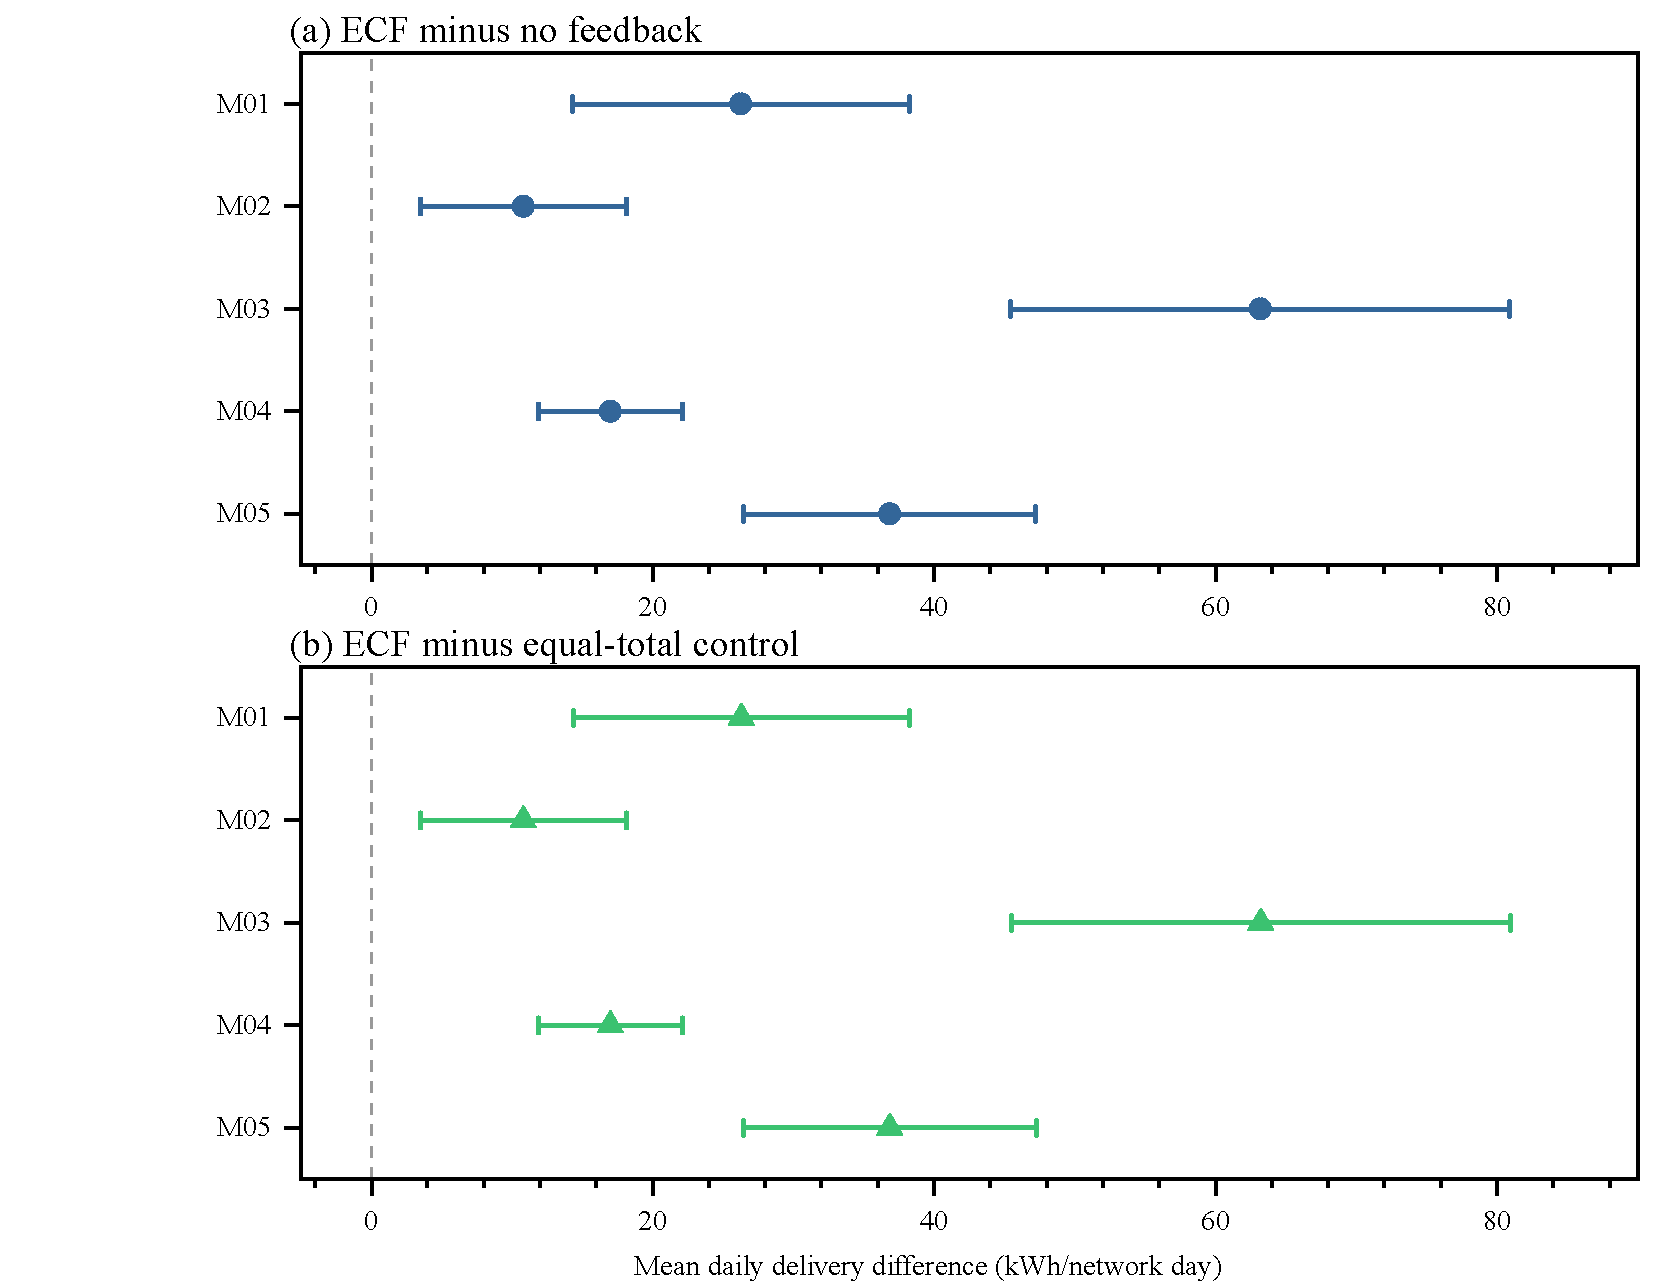
\includegraphics[width=0.75\textwidth]{figures/figS01_profile_mapping.pdf}
\caption{Profile placement changes the mean delivery advantage.
Markers show ECF-minus-control mean modeled delivery per network day,
and horizontal bars show pointwise 95\% intervals adjusted for calendar
dependence. (a) ECF minus no feedback. (b) ECF minus the equal-total control.
Each row uses the same 80 dates under one fixed profile assignment.
The zero line denotes no mean difference. Identical axis scales allow the
two comparisons to be read directly; daily losses remain included in each mean.}
\label{fig:supp_mapping}
\end{figure}

\Needspace{12\baselineskip}

\subsection{PV capacity at fixed participant locations}
\label{supp:pv_capacity}

ECF retains a positive aggregate delivery advantage across five PV capacity
levels, but the advantage does not grow in proportion to installed capacity.
This comparison changes generation capacity at the same participant locations,
complementing the profile-placement comparison in Section~\ref{supp:mapping}.
It also shows that higher delivery can accompany either more or less unused
authorization.

\paragraph{Capacity and matched operating conditions.}
The capacity levels are 0.50, 0.75, 1.00, 1.25, and 1.50 times the primary
scale, corresponding to 2.045--6.135~MW across the 418 export participants.
Gross PV profiles and registered export capacities use the same factor.
Available export is then recalculated after subtracting the unchanged load;
it is not obtained by multiplying the original net surplus. The forecast
rule retains its 90th-percentile increment, recalculated from the scaled
2010--2011 profiles. Previous-day persistence uses the corresponding scaled
profile without that increment.

All levels retain the same participant locations, profile assignment, phase
connections, 80 dates, load multiplier 0.30, feedback gain 0.5, and daily
capacity initialization. The allocation search and physical checks are
unchanged, including the 1.07-pu authorization ceiling, 0.90--1.10-pu delivery
range, and native transformer limits. No feedback, previous-day persistence,
ECF, and each ECF trajectory's own equal-total control are compared within
each capacity level. The four additional factors were fixed before their
simulations, after the primary analysis was available. The original factor
1.00 remains the primary reference.

\paragraph{Delivery, scarcity, and authorization.}
Across all five levels, ECF gains 1.392--1.879~MWh over no feedback and
1.392--1.884~MWh over the equal-total control. The corresponding mean-difference
intervals remain above zero. The primary results are given in
Table~\ref{tab:supp_au_results}; Table~\ref{tab:supp_pv_contrasts} reports
the four added levels. Every level nevertheless includes days on which ECF
delivers less than either control.

The fraction of no-feedback half-hours with a network-limited request scale
rises from 37.0\% to 46.0\% as capacity increases. ECF qualification rises
from 11.5\% to 13.3\%, but its delivery advantage is not monotonic
(Table~\ref{tab:supp_pv_scale}). Gain per installed MW over the 80 dates falls
from 0.813 to 0.273~MWh. Thus more frequent constrained allocation does not
produce a proportionally larger feedback benefit. The constrained-request
fraction counts half-hours with a reduced proportional allocation factor
under the stated search; it does not estimate native hosting capacity.

At factor 0.50, authorization increases by 2.262~MWh and unused authorization
by 0.599~MWh relative to no feedback. Their difference gives the 1.662-MWh
delivery gain. Factors 0.75 and 1.50 also increase unused authorization,
whereas factors 1.00 and 1.25 reduce it. The energy identity accounts for
positive delivery changes with either direction of unused-authorization change;
it does not assign separate causal effects to its two components.
Previous-day persistence leaves less authorization unused at every level but
delivers 47.52--51.94~MWh less than ECF
(Table~\ref{tab:supp_pv_energy}).

\paragraph{Uncertainty and physical checks.}
Each added level uses 80 paired network days. The pointwise 95\% intervals
use 10,000 antithetic dependent wild-bootstrap replicates, with a covariance
that decreases linearly to zero over eight calendar days (random key 184).
The levels share their dates and network and are not pooled as independent
feeder samples. The four added levels contain 61,440 interval--control records
and 15,360 completed-state replay comparisons. All pass the stated numerical,
customer-voltage, and transformer-loading checks. Separate nonlinear AC solves
of the saved replay endpoints give the same physical-check status.
This comparison varies PV size at fixed adoption and does not vary the
number or location of participating connections.

\begin{table}[!htbp]
\centering
\caption{PV capacity, constrained requests, and the ECF-minus-no-feedback
energy balance over 80 dates. Capacity is installed participant PV in MW.
Limited and Qualified are percentages of all 3,840 half-hours: a reduced
allocation factor without feedback and a qualifying ECF replay, respectively.
Authorization, unused authorization, and delivery changes are in MWh.
Gain/MW is additional delivered MWh per installed participant MW over these
dates. Differences use unrounded totals.}
\label{tab:supp_pv_scale}
\small
\begin{tabular}{@{}rrrrrrrr@{}}
\toprule
Factor & Capacity & Limited & Qualified & Authorization & Unused & Delivery & Gain/MW \\
\midrule
0.50 & 2.045 & 37.0 & 11.5 & 2.262 & 0.599 & 1.662 & 0.813 \\
0.75 & 3.067 & 41.9 & 11.9 & 1.882 & 0.003 & 1.879 & 0.612 \\
1.00 & 4.090 & 44.4 & 12.6 & 1.206 & $-0.186$ & 1.392 & 0.340 \\
1.25 & 5.112 & 45.3 & 12.8 & 1.342 & $-0.147$ & 1.488 & 0.291 \\
1.50 & 6.135 & 46.0 & 13.3 & 1.867 & 0.189 & 1.678 & 0.273 \\
\bottomrule
\end{tabular}
\end{table}

\begin{table}[!htbp]
\centering
\caption{Paired delivery comparisons at the four additional PV capacities.
Differences are ECF minus the named control. Mean and pointwise 95\% interval
are in kWh per network day; Total is in MWh over 80 dates. The last column
counts positive, negative, and unchanged daily differences, respectively.
Equal-total denotes the matched proportional request reduction, and
Persistence denotes the previous-day request without the forecast increment.}
\label{tab:supp_pv_contrasts}
\small
\begin{tabular}{@{}rlrrrl@{}}
\toprule
Factor & Control & Mean & 95\% interval & Total & $+/-/0$ days \\
\midrule
0.50 & No feedback & 20.78 & [11.19, 30.37] & 1.662 & 51/28/1 \\
     & Equal-total & 21.31 & [11.82, 30.79] & 1.705 & 51/28/1 \\
     & Persistence & 594.06 & [552.14, 635.97] & 47.524 & 80/0/0 \\
\midrule
0.75 & No feedback & 23.48 & [11.06, 35.91] & 1.879 & 49/31/0 \\
     & Equal-total & 23.55 & [11.13, 35.98] & 1.884 & 49/31/0 \\
     & Persistence & 622.18 & [585.45, 658.91] & 49.774 & 80/0/0 \\
\midrule
1.25 & No feedback & 18.60 & [5.53, 31.67] & 1.488 & 47/29/4 \\
     & Equal-total & 18.61 & [5.54, 31.68] & 1.489 & 48/30/2 \\
     & Persistence & 639.03 & [604.07, 673.98] & 51.122 & 80/0/0 \\
\midrule
1.50 & No feedback & 20.97 & [6.83, 35.11] & 1.678 & 46/32/2 \\
     & Equal-total & 20.97 & [6.83, 35.11] & 1.678 & 47/32/1 \\
     & Persistence & 649.23 & [614.92, 683.55] & 51.939 & 80/0/0 \\
\bottomrule
\end{tabular}
\end{table}

\begin{table}[!htbp]
\centering
\caption{Energy totals at all five PV capacities over the same 80 dates.
All energy columns are in MWh. Unused is authorized minus delivered energy;
negative source exchange denotes net upstream import. The factor-1.00 rows
repeat the unchanged primary reference. All four controls pass the specified
physical checks at every level.}
\label{tab:supp_pv_energy}
\small
\begin{tabular}{@{}rlrrrr@{}}
\toprule
Factor & Control & Authorized & Unused & Delivered & Source exchange \\
\midrule
0.50 & No feedback & 298.696 & 98.512 & 200.183 & $-303.934$ \\
 & Persistence & 184.406 & 30.085 & 154.321 & $-349.520$ \\
 & ECF & 300.957 & 99.111 & 201.846 & $-302.289$ \\
 & Equal-total & 298.406 & 98.264 & 200.141 & $-303.975$ \\
\midrule
0.75 & No feedback & 318.310 & 94.121 & 224.190 & $-276.706$ \\
 & Persistence & 202.295 & 26.001 & 176.294 & $-324.304$ \\
 & ECF & 320.192 & 94.124 & 226.068 & $-274.848$ \\
 & Equal-total & 318.133 & 93.949 & 224.184 & $-276.712$ \\
\midrule
1.00 & No feedback & 328.490 & 90.526 & 237.963 & $-260.959$ \\
 & Persistence & 212.296 & 23.267 & 189.030 & $-309.584$ \\
 & ECF & 329.696 & 90.341 & 239.356 & $-259.582$ \\
 & Equal-total & 328.483 & 90.519 & 237.964 & $-260.959$ \\
\midrule
1.25 & No feedback & 335.183 & 87.949 & 247.234 & $-250.321$ \\
 & Persistence & 218.954 & 21.354 & 197.600 & $-299.639$ \\
 & ECF & 336.524 & 87.802 & 248.722 & $-248.849$ \\
 & Equal-total & 335.164 & 87.931 & 247.233 & $-250.321$ \\
\midrule
1.50 & No feedback & 340.650 & 86.634 & 254.017 & $-242.514$ \\
 & Persistence & 223.567 & 19.811 & 203.756 & $-292.454$ \\
 & ECF & 342.517 & 86.823 & 255.694 & $-240.854$ \\
 & Equal-total & 340.649 & 86.632 & 254.017 & $-242.514$ \\
\bottomrule
\end{tabular}
\end{table}

\Needspace{15\baselineskip}

\subsection{Variation across low-voltage sections of the parent feeder}
\label{supp:au_sections}

ECF delivers more than the equal-total control in all 13 retained LV sections.
Against no feedback, 12 differences are positive and one is negative. Spatial targeting therefore improves on uniform reduction throughout
this panel, but it does not always improve on leaving requests unchanged.

The public collection provides executable models for its nested LV sections. We
retain sections with at least 20 mapped load connections and five export
participants: LV9, LV10, LV11, LV12, LV15, LV17, LV22, LV24, LV25, LV26, LV29,
LV30, and LV32. Each native OpenDSS master model is solved separately. All
sections use the common chronology and scenario of the parent collection.
Their energy differences describe separate section models; the full-feeder
difference is evaluated in the coupled MV/LV model.

Every selected section uses the primary 80-day assessment calendar,
profile-to-service mapping, load scale, allocation-stage upper-voltage ceiling, request model, and
$\beta_{\mathrm{ECF}}=0.5$. Table~\ref{tab:supp_au_lv_sections} reports every
outcome. All 13 sections contain qualifying intervals, and all 199,680
interval--control records pass the specified allocation and modeled-delivery
checks. LV26 alone has a negative total relative to no feedback
($-3.7$~kWh), but gains 71.2~kWh relative to the equal-total control.
Modeled-delivery voltages range from 0.9136 to 1.0952~pu across the panel.
No modeled-delivery state exceeds its native transformer nameplate.

\begin{table}[!ht]
\centering
\caption{Within-collection low-voltage-section outcomes over the 80 assessment
days. Differences are ECF minus the stated control in kWh. The final column
indicates whether all specified allocation and modeled-delivery checks pass
across the four controls.}
\label{tab:supp_au_lv_sections}
\scriptsize
\setlength{\tabcolsep}{3.1pt}
\begin{tabular}{@{}lrrrrrl@{}}
\toprule
Section & Connections & Participants & \shortstack{ECF $-$ no\\feedback} & \shortstack{ECF $-$ equal-total\\control} & \shortstack{Qualifying\\intervals} & \shortstack{All checks\\pass} \\
\midrule
LV9 & 123 & 35 & 844.7 & 873.8 & 580 & Yes \\
LV10 & 94 & 33 & 371.5 & 454.5 & 374 & Yes \\
LV11 & 110 & 41 & 511.7 & 545.2 & 360 & Yes \\
LV12 & 121 & 36 & 1304.5 & 1311.6 & 595 & Yes \\
LV15 & 46 & 12 & 198.2 & 200.3 & 237 & Yes \\
LV17 & 141 & 48 & 107.0 & 287.1 & 308 & Yes \\
LV22 & 21 & 9 & 205.0 & 206.1 & 348 & Yes \\
LV24 & 121 & 44 & 947.0 & 985.5 & 329 & Yes \\
LV25 & 112 & 39 & 718.0 & 783.7 & 505 & Yes \\
LV26 & 94 & 31 & $-3.7$ & 71.2 & 101 & Yes \\
LV29 & 41 & 17 & 54.3 & 83.7 & 73 & Yes \\
LV30 & 151 & 51 & 1213.5 & 1261.4 & 371 & Yes \\
LV32 & 22 & 7 & 95.5 & 99.3 & 273 & Yes \\
\bottomrule
\end{tabular}
\end{table}

\subsection{Variation across representative public low-voltage models}
\label{supp:au_topologies}

The representative-model panel changes the published LV topology rather than
the location within one parent feeder. Six of nine eligible models contain
qualifying intervals and show positive aggregate delivery differences against
both controls. All nine models pass the specified physical checks. Models L,
N, and O have no qualifying intervals and no delivery change.

The panel begins with the 23 representative Australian LV models released by
the National Low-Voltage Feeder Taxonomy Study
\cite{geth2021lvtaxonomy}. Eligibility is determined from structure and a
connection-voltage check with mapped household injections set to zero. A retained
model must converge and satisfy the voltage criterion on every declared
connection phase, and it must have a usable native transformer nameplate. It
must also contain at least 20 mapped load premises and five export participants.

The phase-preserving representation retains each published load element as one
allocation premise. It preserves the one-, two-, or three-phase connection and
checks voltage on every declared phase. These criteria select G, J, L, M, N, O,
P, Q, and R. Models A--F, H, I, K, and S lack a native transformer with a
usable nameplate. Models T, U, and V do not meet the size rule. Model W violates
the zero-injection connection-voltage criterion.

Each selected model receives the same 80 observed dates, deterministic profile
assignment, request construction, load scale, allocation-stage upper-voltage ceiling, four
controls, and $\beta_{\mathrm{ECF}}=0.5$. The published model supplies each topology, its connection structure, and
its native equipment data. Table~\ref{tab:supp_au_taxonomy} reports every selected
model. Because the models represent distinct structures rather than a sampled
population, results are interpreted model by model and are not pooled.

\begin{table}[!ht]
\centering
\caption{Results for the public representative-LV-model panel over the 80
assessment days. Differences are ECF minus the named control in kWh.
Every model passes the specified allocation, customer-voltage, and native
transformer checks. Small positive differences are retained rather than
rounded to zero.}
\label{tab:supp_au_taxonomy}
\scriptsize
\setlength{\tabcolsep}{2.7pt}
\begin{tabular}{@{}lrrrrrrr@{}}
\toprule
Model & Conn. & \shortstack{Premise\\phase counts} & \shortstack{ECF $-$ no\\feedback} & \shortstack{ECF $-$ equal-total\\control} & \shortstack{Qualifying\\intervals} & \shortstack{All physical\\checks pass} & \shortstack{Min. voltage\\(pu)} \\
\midrule
G & 59 & 1 & 11.4 & 43.5 & 69 & Yes & 0.9749 \\
J & 87 & 1 & 543.0 & 611.7 & 328 & Yes & 0.9412 \\
L & 36 & 1 & 0.0 & 0.0 & 0 & Yes & 0.9792 \\
M & 58 & 1,3 & 0.1 & 1.3 & 2 & Yes & 0.9662 \\
N & 63 & 1,3 & 0.0 & 0.0 & 0 & Yes & 0.9734 \\
O & 83 & 1,2 & 0.0 & 0.0 & 0 & Yes & 0.9823 \\
P & 109 & 1,2,3 & 58.1 & 145.9 & 85 & Yes & 0.9734 \\
Q & 109 & 1,3 & 960.5 & 982.1 & 685 & Yes & 0.9384 \\
R & 144 & 1,2 & 92.1 & 153.7 & 97 & Yes & 0.9594 \\
\bottomrule
\end{tabular}
\end{table}

\subsection{Individual delivery changes under shared constraints}
\label{supp:individual_delivery}

The primary aggregate gain is shared unevenly. Relative to no feedback,
330 of the 418 participant connections gain cumulative delivery and 88 lose
delivery over the 80 assessed days. The positive changes sum to 1.557~MWh
and the negative changes to $-0.165$~MWh, leaving the reported net gain of
1.392~MWh. The median individual change is 2.6~kWh and the largest loss
is 7.3~kWh. The equal-total comparison has the same participant counts
and a similar distribution (Table~\ref{tab:supp_individual_delivery}).

Each individual difference sums ECF-minus-control delivery over the same
half-hours. The comparison with the same update without replay qualification
instead gives 417 positive individual totals and one negative total of
$-1.17$~kWh. Thus retaining qualification benefits more participants than
updating after every unused award, but does not make every participant
better off than no feedback.

Positive cumulative delivery also does not imply a benefit on every day.
All 418 participants have at least one negative day against no feedback or
the equal-total control. The longest uninterrupted run of negative daily
differences is five days against either control. A missing calendar date
breaks a run; separated assessment days are not treated as consecutive.
The corresponding maximum against the update without qualification is
seven days. These statistics describe observed model trajectories, not
participant-level causal responsibility or financial losses.

\begin{table}[!htbp]
\centering
\caption{Individual delivery differences in the primary 80-day comparison.
All differences are ECF minus the named control. Energy rows are in kWh per
participant unless stated otherwise. Counts cover all 418 participant
connections. The last column uses the same ceiling update without replay
qualification. Day-run statistics break at gaps in the assessment calendar.}
\label{tab:supp_individual_delivery}
\small
\begin{tabular}{@{}p{6.0cm}rrr@{}}
\toprule
 & No feedback & Equal-total & No qualification \\
\midrule
Positive cumulative difference & 330 & 330 & 417 \\
Negative cumulative difference & 88 & 88 & 1 \\
Unchanged cumulative difference & 0 & 0 & 0 \\
Minimum individual difference & $-7.31$ & $-7.31$ & $-1.17$ \\
5th percentile & $-2.83$ & $-2.83$ & 3.07 \\
25th percentile & 0.43 & 0.43 & 7.70 \\
Median & 2.60 & 2.60 & 12.57 \\
75th percentile & 5.09 & 5.09 & 19.86 \\
95th percentile & 13.52 & 13.52 & 36.06 \\
Maximum individual difference & 30.50 & 30.50 & 124.38 \\
Participants with any negative day & 418 & 418 & 417 \\
Maximum negative-day count & 34 & 36 & 36 \\
Longest consecutive negative-day run & 5 & 5 & 7 \\
\bottomrule
\end{tabular}
\end{table}

\subsection{Requests adjusted from participants' own delivery}
\label{supp:experiential_requests}

We test whether delivery comparisons change when participants revise their
requests after observing their own completed delivery. Each of the 418 export
participants chooses among five multipliers,
$m_k\in\{0.50,0.75,1.00,1.25,1.50\}$, where $k=1,\ldots,5$.
These choices allow both smaller and larger requests. They are distinct from
the optimal larger-request multiplier $\gamma_i^\star$ in the controlled study.
Let $r_i^{\mathrm{base}}(t)$ denote the capacity-capped, history-based request
used by the primary public-data simulation before any feedback ceiling is
applied. If participant $i$ selects candidate $k$, its capacity-capped request is
\begin{equation}
 r_i^{\mathrm{cap}}(t)=\min\{C_i,m_k r_i^{\mathrm{base}}(t)\}.
 \label{eq:supp_experiential_request}
\end{equation}
The applicable request ceiling and the original allocation rule then determine
admitted requests and awards. The network, profile mapping, PV capacity,
feedback formula, and nominal gain remain unchanged.

We use the Exp3 preference update of Auer et al., which raises the selection weight of a candidate after a larger
normalized delivery reward.\cite{Auer2002Exp3}
Let $w^{\mathrm{req}}_{ik}(t)>0$ denote participant $i$'s preference weight for candidate $k$,
and let $p^{\mathrm{req}}_{ik}(t)$ denote its selection probability. The weights start at one,
and selection uses
\begin{equation}
 p^{\mathrm{req}}_{ik}(t)=0.90\frac{w^{\mathrm{req}}_{ik}(t)}{\sum_{h=1}^{5}w^{\mathrm{req}}_{ih}(t)}+\frac{0.10}{5}.
 \label{eq:supp_experiential_probability}
\end{equation}
After delivery is completed, only the selected candidate's weight is updated:
\begin{equation}
 w^{\mathrm{req}}_{ik}(t+1)=w^{\mathrm{req}}_{ik}(t)
 \exp\!\left[\frac{0.10}{5p^{\mathrm{req}}_{ik}(t)}\frac{y_i(t)}{C_i}\right].
 \label{eq:supp_experiential_update}
\end{equation}
Other weights are unchanged. Computation uses logarithmic weights and a common
row normalization, which leaves the probabilities unchanged. Zero baseline
requests produce zero delivery and no preference update. The reward is the
participant's own delivered power divided by its connection bound, consistent
with the primary zero-shortfall-cost setting. Request selection does not use
current available export, other participants' private information, or replay
outcomes. A comparison with no preference update retains the same initial
probabilities and random draws but leaves all weights unchanged.

No feedback, ECF, and the same update without qualification each have their own
delivery histories and evolving preferences. Their contrasts therefore include
subsequent request responses. The equal-total shadow instead follows ECF's
history and current capacity-capped requests, removing the same total request at that
interval. Its contrast retains the conditional comparison of where requests
are reduced; it is not the trajectory of an independently adapting uniform
controller.

Both preferences and ceilings persist across midnight within each of the ten
consecutive-date blocks. They are initialized again after calendar gaps; the
longest block spans 35 days. Each behavior mode uses seeds 2001, 2002, and 2003,
fixed before evaluation. We retain every seed and date, first averaging the
three seeds within each date for the main paired comparisons. Uncertainty is
computed over the original 80 dates with the same calendar-dependent procedure
used for the other public-data comparisons. The 480 setting-days do not extend
the observed calendar. Seed-specific and block-level contrasts accompany the
date-averaged results.

This participant model tests experience-based request adjustment. It does not
model strategies that anticipate future ceilings or manipulate availability
records. Exp3's regret guarantees are not transferred to the coupled allocation
and feedback system.


Preference adjustment preserves ECF's aggregate delivery advantage
(Fig.~\ref{fig:supp_request_adaptation} and
Table~\ref{tab:supp_adapt_contrasts}). Relative to no feedback, the mean
gain is 18.1~kWh per day (95\% interval 10.5--25.6), or 1.44~MWh over the
80 dates. The gain over the same update without qualification is
56.6~kWh per day (46.0--67.3), or 4.53~MWh. All three seeds give positive
mean contrasts, although individual dates and consecutive-date blocks can
lose delivery. ECF exceeds the conditional equal-total shadow by
1.50~MWh. This last comparison holds ECF's request history fixed; the first
two include the separate histories produced by each controller.

The energy balance explains why lower unused authorization is not the sole
source of benefit (Table~\ref{tab:supp_adapt_energy}). Against no feedback,
ECF grants 1.31~MWh more authorization and leaves 0.14~MWh less unused,
together delivering 1.44~MWh more. Against updating without qualification,
it grants 20.99~MWh more authorization and leaves 16.46~MWh more unused.
The remaining 4.53~MWh reaches delivery. Thus a controller can suppress
unused authorization more aggressively while also removing useful awards.

Preference adjustment changes the requests passed to allocation. Their time
integral under ECF is 1656.33~MWh, compared with 1629.26~MWh at fixed
probabilities, after averaging the three seeds.
This integral measures requests over time, not awarded or delivered energy.
To isolate the effect of preference updates, the comparison keeps the candidate
requests and random draws unchanged. A direct comparison with the primary
forecast-based request would change both the candidate set and the preference
update.

Table~\ref{tab:supp_adapt_interaction} compares ECF's advantage between these
two behavior modes. Preference adjustment increases its daily advantage
over no feedback by 0.58~kWh, with a 95\% interval of $-0.58$ to 1.73.
For the conditional equal-total shadow, the increase is 1.22~kWh
($-0.02$ to 2.45). Neither interval resolves an increase above zero.
In contrast, the advantage over updating without qualification increases
by 5.68~kWh per day (2.54--8.83). The results therefore support persistence
of ECF's mean advantage under experience-based request adjustment, rather
than a general claim that adaptation amplifies it.

The six behavior-mode and seed combinations contain 92,160
interval--control records and 23,040 replay states. Independent AC
re-evaluation of the saved states confirms the specified customer-voltage
and transformer-loading checks throughout. These checks establish physical
feasibility, not positive delivery changes on every date.
Table~\ref{tab:supp_adapt_blocks} retains the positive and negative block
contrasts. All date- and seed-level results accompany the plotting data.
The pointwise 95\% intervals use the covariance in
\eqref{eq:supp_au_wild_covariance}, with 10,000 antithetic draws and seed
189; they do not adjust for multiple comparisons.

\begin{figure}[!htbp]
\centering
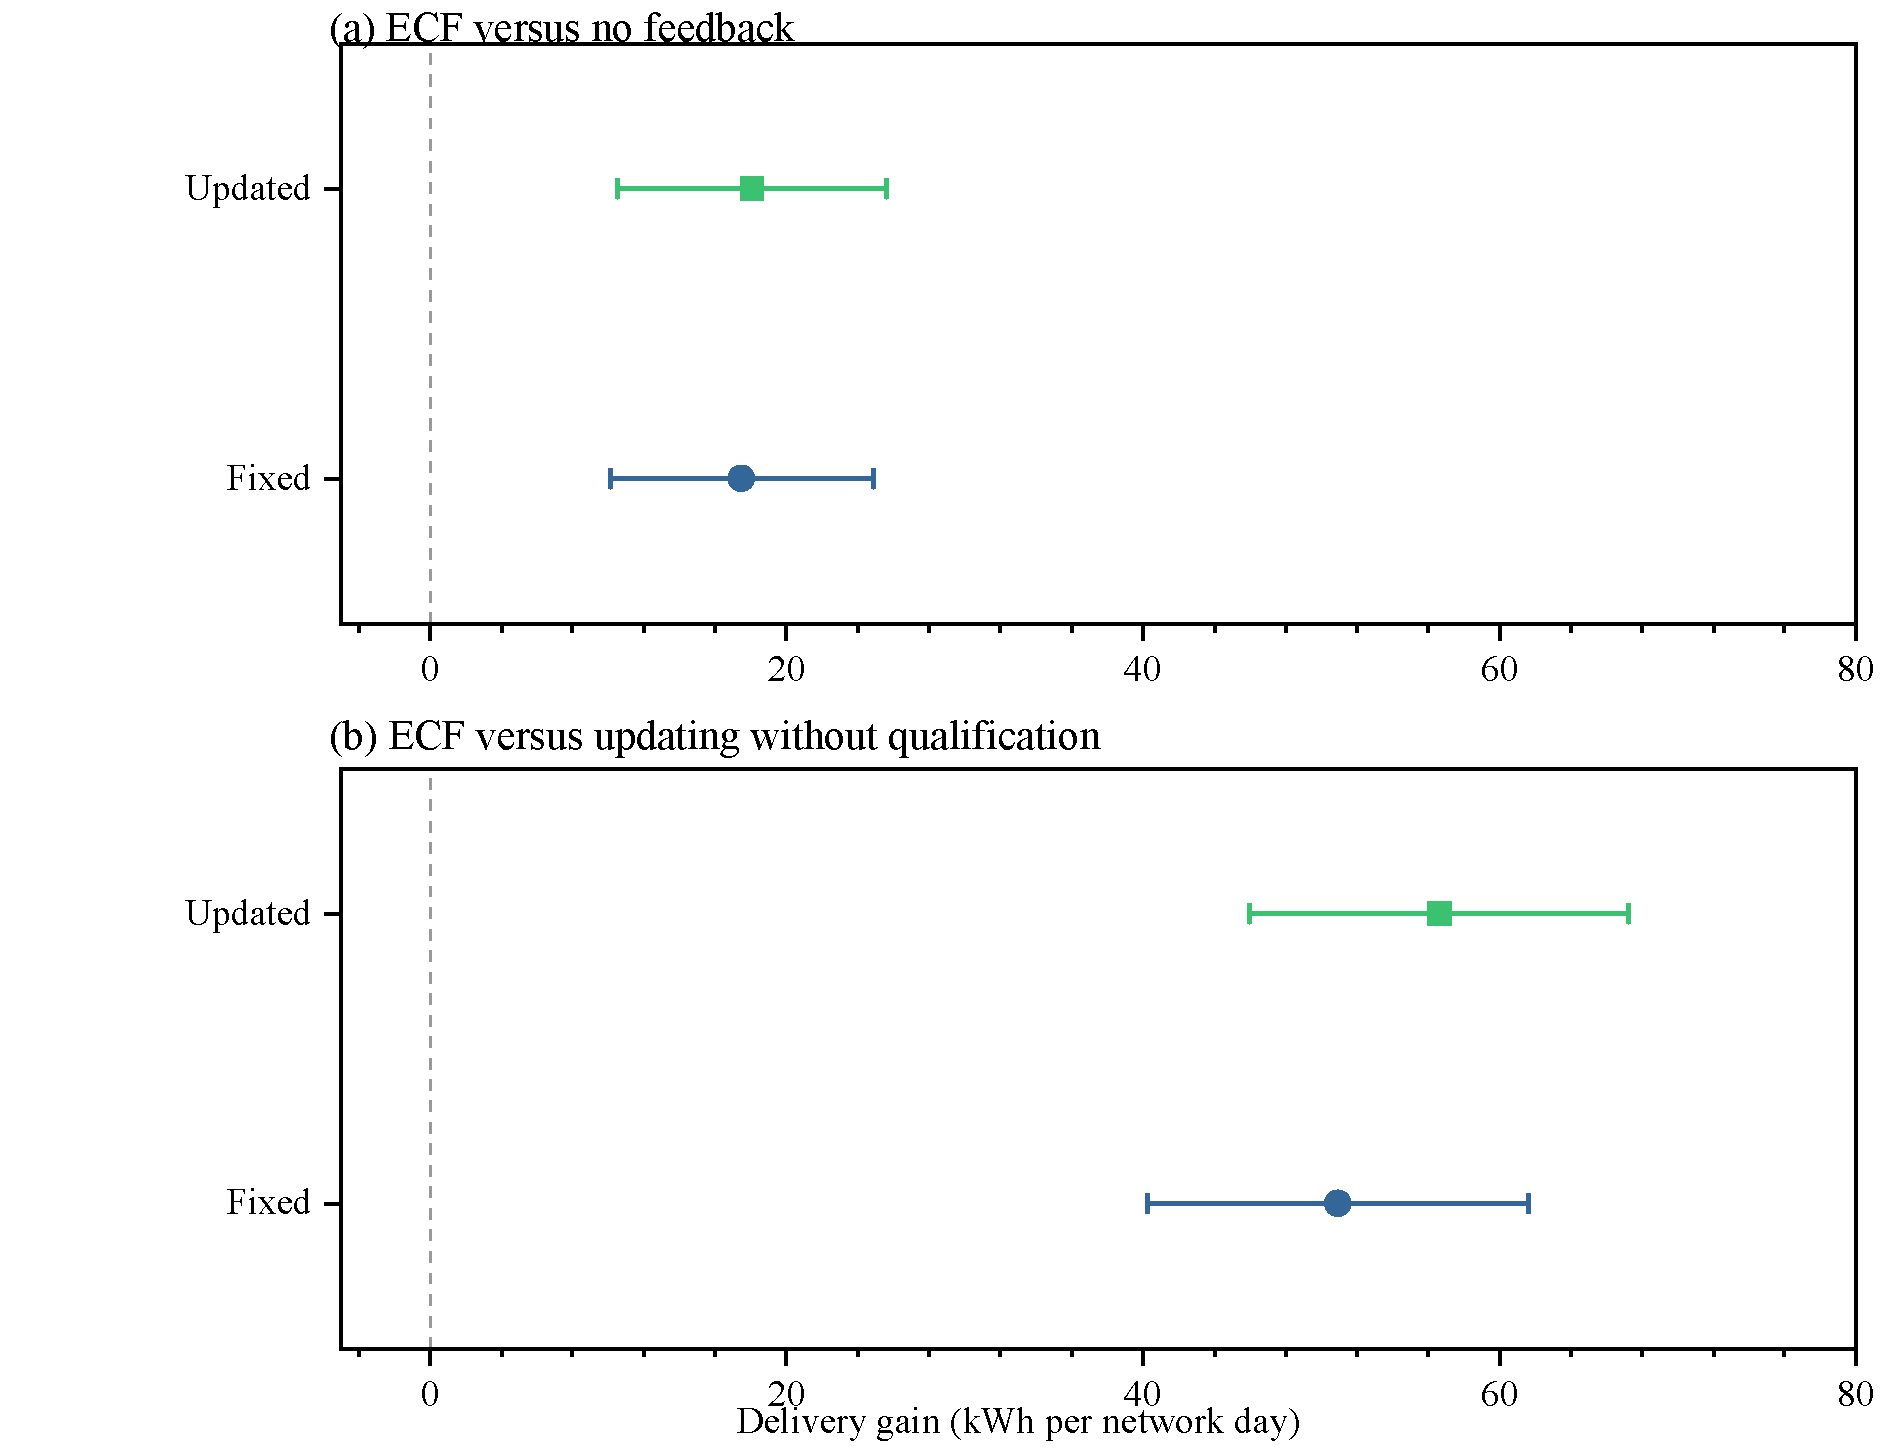
\includegraphics[width=0.86\textwidth]{figures/figS02_request_adaptation.pdf}
\caption{Delivery gains with fixed and updated request-choice probabilities.
ECF is compared with (a) no feedback and (b) the same ceiling update without
replay qualification. Blue circles denote fixed probabilities; green squares
denote probabilities updated from each participant's own completed delivery.
Both modes randomly select among the same candidate requests. Markers show
mean daily differences after averaging the three seeds within each of the
80 dates. Horizontal bars show pointwise 95\% intervals accounting for
calendar dependence. The panels share the same horizontal scale. Each
controller maintains its own request and delivery history.
Table~\ref{tab:supp_adapt_interaction} reports the paired change in ECF's
advantage between the two request-choice modes.}
\label{fig:supp_request_adaptation}
\end{figure}

\begin{table}[!htbp]
\centering
\caption{Delivery gains under updated and fixed request-choice probabilities. All differences are ECF minus the named control. Mean and pointwise 95\% interval are in kWh per network day; Total is in MWh over 80 dates. Mean-seed rows average the three seeds within each date before aggregation. The last column counts positive, negative, and unchanged dates. The equal-total shadow follows ECF's request history.}
\label{tab:supp_adapt_contrasts}
\small
\begin{tabular}{@{}lllrrrl@{}}
\toprule
Probabilities & Control & Seed & Mean & 95\% interval & Total & $+/-/0$ days \\
\midrule
Updated & No feedback & 2001 & 13.21 & [5.61, 20.81] & 1.057 & 43/37/0 \\
Updated & No feedback & 2002 & 21.66 & [11.70, 31.61] & 1.733 & 51/28/1 \\
Updated & No feedback & 2003 & 19.29 & [9.98, 28.60] & 1.543 & 51/29/0 \\
Updated & No feedback & Mean & 18.05 & [10.52, 25.59] & 1.444 & 54/26/0 \\
Updated & Without qualification & 2001 & 57.49 & [46.59, 68.38] & 4.599 & 71/9/0 \\
Updated & Without qualification & 2002 & 56.27 & [43.10, 69.44] & 4.502 & 67/13/0 \\
Updated & Without qualification & 2003 & 56.11 & [43.56, 68.66] & 4.489 & 71/9/0 \\
Updated & Without qualification & Mean & 56.62 & [45.98, 67.26] & 4.530 & 73/7/0 \\
Updated & Equal-total shadow & 2001 & 13.83 & [6.05, 21.60] & 1.106 & 44/36/0 \\
Updated & Equal-total shadow & 2002 & 22.58 & [12.52, 32.64] & 1.806 & 51/28/1 \\
Updated & Equal-total shadow & 2003 & 19.67 & [10.36, 28.98] & 1.574 & 53/26/1 \\
Updated & Equal-total shadow & Mean & 18.69 & [11.02, 26.37] & 1.495 & 55/25/0 \\
Fixed & No feedback & 2001 & 13.62 & [5.10, 22.13] & 1.089 & 48/32/0 \\
Fixed & No feedback & 2002 & 21.04 & [11.17, 30.90] & 1.683 & 49/30/1 \\
Fixed & No feedback & 2003 & 17.78 & [9.58, 25.98] & 1.422 & 50/29/1 \\
Fixed & No feedback & Mean & 17.48 & [10.12, 24.84] & 1.398 & 54/26/0 \\
Fixed & Without qualification & 2001 & 53.26 & [42.24, 64.28] & 4.261 & 69/11/0 \\
Fixed & Without qualification & 2002 & 50.35 & [36.27, 64.44] & 4.028 & 64/16/0 \\
Fixed & Without qualification & 2003 & 49.20 & [35.95, 62.44] & 3.936 & 68/12/0 \\
Fixed & Without qualification & Mean & 50.94 & [40.27, 61.60] & 4.075 & 74/6/0 \\
Fixed & Equal-total shadow & 2001 & 13.62 & [5.10, 22.13] & 1.089 & 48/32/0 \\
Fixed & Equal-total shadow & 2002 & 21.04 & [11.18, 30.90] & 1.683 & 49/30/1 \\
Fixed & Equal-total shadow & 2003 & 17.77 & [9.57, 25.97] & 1.422 & 50/29/1 \\
Fixed & Equal-total shadow & Mean & 17.48 & [10.12, 24.84] & 1.398 & 54/26/0 \\
\bottomrule
\end{tabular}
\end{table}

\begin{table}[!htbp]
\centering
\caption{Energy totals under the two request-choice modes, averaged over the three seeds. All entries are MWh over the same 80 dates. Unused equals authorized minus delivered energy; negative source exchange denotes net upstream import. Differences are calculated before rounding.}
\label{tab:supp_adapt_energy}
\small
\begin{tabular}{@{}llrrrr@{}}
\toprule
Probabilities & Control & Authorized & Unused & Delivered & Source exchange \\
\midrule
Updated & No feedback & 311.55 & 85.90 & 225.65 & -273.21 \\
Updated & ECF & 312.86 & 85.76 & 227.09 & -271.78 \\
Updated & Without qualification & 291.86 & 69.30 & 222.56 & -276.27 \\
Updated & Equal-total shadow & 311.44 & 85.85 & 225.60 & -273.26 \\
Fixed & No feedback & 308.81 & 84.78 & 224.03 & -274.82 \\
Fixed & ECF & 310.08 & 84.66 & 225.43 & -273.43 \\
Fixed & Without qualification & 290.06 & 68.71 & 221.35 & -277.48 \\
Fixed & Equal-total shadow & 308.79 & 84.77 & 224.03 & -274.82 \\
\bottomrule
\end{tabular}
\end{table}

\begin{table}[!htbp]
\centering
\caption{Change in ECF's delivery advantage when request-choice probabilities are updated rather than fixed. Each entry is the updated-probability ECF-minus-control contrast minus its fixed-probability counterpart, with seeds averaged within each date. Mean and pointwise 95\% interval are in kWh per day; Total is MWh over 80 dates.}
\label{tab:supp_adapt_interaction}
\small
\begin{tabular}{@{}lrrrl@{}}
\toprule
Control & Mean & 95\% interval & Total & $+/-/0$ days \\
\midrule
No feedback & 0.58 & [-0.58, 1.73] & 0.046 & 36/44/0 \\
Without qualification & 5.68 & [2.54, 8.83] & 0.455 & 57/23/0 \\
Equal-total shadow & 1.22 & [-0.02, 2.45] & 0.097 & 38/42/0 \\
\bottomrule
\end{tabular}
\end{table}

\begin{table}[!htbp]
\centering
\caption{Delivery contrasts within every consecutive-date block. Entries are kWh, ECF minus each control, averaged over three seeds. Block numbering follows chronological order in Section S10.8. Preference weights and ceilings persist within a block and restart after calendar gaps; gains need not be positive in every block.}
\label{tab:supp_adapt_blocks}
\small
\begin{tabular}{@{}lrrrrr@{}}
\toprule
Probabilities & Block & Days & No feedback & Without qualification & Equal-total shadow \\
\midrule
Updated & 1 & 7 & 35.02 & 122.20 & 38.27 \\
Updated & 2 & 14 & 165.85 & 634.78 & 163.67 \\
Updated & 3 & 3 & 64.87 & 367.70 & 65.54 \\
Updated & 4 & 2 & 93.28 & -13.94 & 92.85 \\
Updated & 5 & 2 & -18.23 & 35.51 & -16.58 \\
Updated & 6 & 1 & 0.02 & 89.51 & -1.31 \\
Updated & 7 & 4 & 1.72 & 258.17 & 3.96 \\
Updated & 8 & 7 & 215.44 & 322.15 & 215.98 \\
Updated & 9 & 35 & 802.90 & 2297.81 & 849.63 \\
Updated & 10 & 5 & 83.43 & 415.83 & 83.47 \\
Fixed & 1 & 7 & 45.17 & 116.09 & 45.15 \\
Fixed & 2 & 14 & 133.45 & 543.69 & 133.58 \\
Fixed & 3 & 3 & 65.71 & 362.56 & 65.70 \\
Fixed & 4 & 2 & 92.64 & -16.96 & 92.63 \\
Fixed & 5 & 2 & -15.66 & 35.30 & -15.66 \\
Fixed & 6 & 1 & 0.84 & 90.30 & 0.83 \\
Fixed & 7 & 4 & 2.38 & 251.95 & 2.35 \\
Fixed & 8 & 7 & 230.79 & 323.76 & 230.80 \\
Fixed & 9 & 35 & 763.97 & 1959.77 & 763.96 \\
Fixed & 10 & 5 & 78.84 & 408.59 & 78.83 \\
\bottomrule
\end{tabular}
\end{table}

% Keep the adaptation figure and result tables before the closing interpretation.
\FloatBarrier
\subsection{Interpretation and scope}
\label{supp:au_scope}

The public analyses distinguish the amount of access granted, the electricity
delivered, and the reliability of the comparison used to update requests.
The primary energy balance and equal-total comparison show that delivery
can increase without a reduction in total authorization. The same-update
comparison identifies the value of qualifying an unused-award episode.
Gain, memory, and bounded-record analyses then distinguish a valid reason to
update from the energy value of the later response. Spatial and behavioral
comparisons show how these outcomes change when profile placement, available
generation, network structure, or participants' request histories change.

The original 30 public-data cases contain 514,752 interval--control records:
15,360 primary, 92,160 gain/record-sensitivity, 69,312 complete-cohort,
199,680 nested-section, and 138,240 representative-model records. All pass the
specified allocation and delivery checks. Sections~\ref{supp:same_update_qualification},
\ref{supp:contiguous_state}, \ref{supp:bounded_record_dynamic},
\ref{supp:mapping}, \ref{supp:pv_capacity}, and \ref{supp:experiential_requests}
report the coverage of the further matched comparisons. These counts describe
evaluated states, including repeated dates and reused control trajectories;
they are not independent feeder samples. Statistical comparisons use paired
network days, with seeds averaged within dates in the request-adaptation study.

The controlled case tests voltage, power balance, and two-ended apparent power
against synthetic medium-voltage ratings. The Australian models instead supply
customer-voltage limits and transformer nameplates, without usable native line
ampacities. Their physical results refer to those specified checks. The
constructed profile mapping, requests, and available-export proxy are common
assumptions of the public analyses. Source-terminal accounting follows the
delivery change through a feeder that remains a net importer.

Field evaluation requires linked operating records and longer participant and
controller histories. Experience-based request adjustment does not represent
anticipation of future ceilings or manipulation of availability records.
Likewise, fixed participant locations in the placement and PV-capacity studies
do not test changing adoption. The energy gain must be assessed against record
validation, communication, and computation costs. Annual energy, welfare,
market value, generation displacement, and emissions require the corresponding
calendar coverage and economic or emissions models. The repository contains
source identifiers, preprocessing and mapping, chronological roles, result
tables, statistics, network-endpoint quantities, and analysis code. Its
reproduction instructions distinguish verification of saved tables from full
simulation reruns and identify the external inputs and auxiliary trajectory
caches required by the archived diagnostic programs.


\begingroup
\footnotesize
\bibliographystyle{rsc}
\bibliography{references}
\endgroup

\end{document}
